\documentclass{report}

%--------------------------------------------------- PAGE STYLE 
\usepackage[utf8]{inputenc} 		% Encoding
\usepackage[T1]{fontenc} 			% To write in French
\usepackage[english]{babel} 			% To write in English
\usepackage{fancyhdr} 				% Fancy style
\usepackage[left=1.7cm,right=1.7cm,top=1.7cm,bottom=1.7cm]{geometry}
\usepackage[titletoc]{appendix}	   	% Better appendix management
\usepackage[absolute]{textpos}
\usepackage{booktabs}
\usepackage{etoolbox}					% Manage toclof lines

\usepackage{expdlist}
\newenvironment{itemize*}%			% Creates a custom itemize environment, called by itemize* 
  {\begin{itemize}%
    \setlength{\itemsep}{0pt}%		% The interline is reduced so that we don't waste space
    \setlength{\parskip}{0pt}}%
  {\end{itemize}}
  
\renewcommand{\rmdefault}{phv}	% Use Helvetica as default font for the whole document

\setlength{\parindent}{0pt}	      	% Remove auto-ident

%--------------------------------------------------- COOL CHAPTER NUMBERING
\usepackage{titlesec, blindtext, color}

\titlespacing*{\chapter}{0pt}{0pt}{20pt}	% Remove space used by the "chapter" header

\definecolor{black}{gray}{0}
\newcommand{\hsp}{\hspace{20pt}}
\titleformat{\chapter}[hang]{\LARGE\bfseries}{\thechapter\hsp\textcolor{black}{|}\hsp}{0pt}{\LARGE\bfseries}

%--------------------------------------------------- BIBLIOGRAPHY 
\usepackage{natbib}

%--------------------------------------------------- MATHS STUFF 
\usepackage{float}						% For float
\usepackage{amsmath,amscd,amssymb,epsfig}  %sci equations
\usepackage{matlab-prettifier}      % MATLAB codes
\usepackage[numbered,framed]{mcode} % For MATLAB code
\usepackage{verbatim}               	% to quote code
\usepackage{listings}               	% Include the listings-package
\usepackage{lipsum}					% Cite code
\usepackage{tocloft}					% Different codes inputs manager (python, SciLab, ...)

%--------------------------------------------------- INCLUSIONS 
\usepackage{array}						% Required for tabulars 
\usepackage{graphicx} 				% Required for the inclusion of images
\usepackage[format=plain,
			font={small},
			labelfont={bf,it},
			textfont=it]{caption}   		% To include captions (small, figure in bold, all text in italic)
\usepackage{enumitem}              	% To make lists
\usepackage{url}                    		% to quote URLs
\usepackage{pdfpages}			    % To include PDFs (annexes)
\usepackage{textcomp}		        % For copyright symbol
\usepackage{hyperref}					% To make references 
\usepackage{movie15}					% To include gifs
\usepackage{circuitikz}					% To include circuits

%--------------------------------------------------- TODOs / DRAFT MODE
 
\newif\ifdraft
\drafttrue
%\draftfalse

\ifdraft
\usepackage{todonotes}
\else
\usepackage[disable]{todonotes}
\fi

%--------------------------------------------------- CUSTOM COMMANDS
\newcommand{\ts}{\textsuperscript} 	% Simplifies superscript
\newcommand{\tsb}{\textsubscript}  	% Simplifies subscript


\newcommand{\listequationsname}{List of Equations}		% Create list of equations
\newlistof{myequations}{equ}{\listequationsname}
\newcommand{\myequations}[1]{%
  \refstepcounter{myequations}%
  \addcontentsline{equ}{myequations}
    {\protect\numberline{\theequation}#1}\par%
}
\makeatletter
	\preto\chapter{\addtocontents{equ}{\protect\addvspace{10\p@}}}%	% Set skips between chapters
\makeatother
\setlength{\cftmyequationsnumwidth}{2.5em} % Width of equation number in List of Equations
\setlength{\cftmyequationsindent}{1.5em}   % Indent of list of equation 

\hbadness=99999  % or any number >=10000
\hfuzz=3pt

\begin{document}

%---------------------------------------------------------------------
%	TITLE PAGE
%---------------------------------------------------------------------

\begin{titlepage}

\newcommand{\HRule}{\rule{\linewidth}{0.5mm}} % horizontal lines

\center % Center everything on the page


\includegraphics[scale=0.4]{logo.png} \\[3cm] % Logo

	%	HEADING 

\textsc{\large International Master Degree in Electro-Acoustics, 2\ts{nd} Year internship report}\\[0.4cm] % Major heading 
\textsc{\normalsize Academic year 2017 - 2018}\\[0.7cm] % Minor heading 

	%	TITLE 

\HRule \\[0.4cm]
 { \huge \bfseries Near-Field Scanner: measurement optimization}\\[0.3cm] 
\HRule \\[1.5cm]

	% DATE
    
{\large \today}\\[2cm] 

	%	AUTHORS - SUPERVISORS

\begin{minipage}{0.4\textwidth}
\begin{flushleft} \large
\emph{Author:}\\ % Author(s)
Chlo\'{e} \textsc{Corno}

\end{flushleft}
\end{minipage}
~
\begin{minipage}{0.4\textwidth}
\begin{flushright} \large
\emph{Referees:} \\ % Supervisor(s) 
\textit{Academic:} Manuel Melon \\
\textit{Company:} Christian Bellmann \\

%\emph{Reviewer:} \\ % Reviewer Name

\end{flushright}
\end{minipage}\\[2cm]
 
\todo[inline, color=red]{DISABLE DRAFT MODE!!!!!!!!!!!!!!!!!!!!!!!!!!!!!!!!!!!!!!!!!!!!!!}
\vfill % Fill the rest of the page with white

\end{titlepage}

%---------------------------------------------------------------------
%	LIST OF TODOS - THANKS
%---------------------------------------------------------------------




%If in draft mode Acknowledgements will not be shown, but the list of todos will
\ifdraft
\listoftodos
%If not in draft mode, Acknowledgements are shown and list of tods is removed
\else
\thispagestyle{empty}
\begin{center}
{\Large\textbf{Acknowledgements}} 
\end{center}
\vspace{1cm}
I would first like to thanks my supervisor Chrisitan Bellmann for all the help and support he provided me during these 5 months. 

\vspace{0.5cm}

I want to particularly thanks the Université du Mans and all the professors and supervisors for giving me the opportunity to follow the Internal Master Degree in ElectroAcoustics and allowing me to work in a domain that passionate me. 

\vspace{0.5cm}

Finally, I want to express my profound gratitude to my family, who supported me during my studies. I would've never made it without you. Thank you.

\vfill % Fill the rest of the page with white
\fi	% End of condition

%---------------------------------------------------------------------
%	TABLE OF CONTENTS - LIST OF FIGURES
%---------------------------------------------------------------------
\pagenumbering{alph} % alpha page numbering for ToC and LoF

\clearpage
	% Change the name of table of contents and other lists
\renewcommand\contentsname{Table of contents}
\tableofcontents
\addtocontents{toc}{~\hfill\textbf{Page}\par} % Adds "page" on top of page number

\clearpage
\listoffigures
\addcontentsline{toc}{chapter}{List of Figures}

\clearpage
\listofmyequations
\addcontentsline{toc}{chapter}{List of Equations}

%--------------------------------------------------------------
%	CODE SAMPLES
%--------------------------------------------------------------

	% IMAGE WITHOUT FLOAT 
    
%\begin{center}
%\includegraphics[width=\textwidth]{name_of_figure} 
%\captionsetup{hypcap=false} 
%\captionof{figure}{some caption for the figure} 
%\label{fig:name_of_label}
%\end{center}

	% ADD CONTENT TO ToC 
    
%\addcontentsline{toc}{[type]}{[Name]}
% type : chapter section subsection ...?
% Name : introduction, ...?


%--------------------------------------------------------------
%	INTRODUCTION
%--------------------------------------------------------------

\chapter*{Introduction}
\addcontentsline{toc}{chapter}{Introduction}
\pagenumbering{arabic} % Arabic page numbering for text corpus


"\textit{What defines a good measurement of a speaker?}" is a common rhetorical question for anyone working in the field of electroacoustics. While purely electrical measurements such as the impedance are quite immune to noise, they do not allow to fully characterize a driver, and acoustical measurements must be conducted. \\
A popular acoustical measurement for loudspeakers is the directivity: allowing to see how a driver radiates at a given angle, this measurement is usually done using one or an array of microphones, and by placing the Device Under Test on a turntable. By rotating the Device Under Test and measuring its SPL response for several angles, the directivity of the device is measured. \\

Although this method is widely used, it presents several drawbacks:
\begin{itemize}
\item Resolution: the higher the angular resolution, the better the measurement but the longer it takes. 
\item Accuracy: a good measurement must ideally be performed in an anechoic room, and in the far field of the Device to avoid any near field effects such as diffraction and interferences.
\item Price: the materials required such as an anechoic room or a performant microphone array can either very expansive or difficult to access. 
\end{itemize}


\todo[inline, color=red!40]{Finir de rédiger l'introduction}

The following reports aims to present the work that have been conducted during a 5-months internship at the company Klippel GmbH. This internship is mandatory to graduate from the International Master Degree in Electro-Acoustics (IMDEA) at the Université du Mans, in France. \\

This document will cover different points, starting with a preface presenting the company, the context and aim of this work, and a literature review. Then the different measurements and results obtained during this work will be presented by using three topic: measurement of devices mounted in baffle, optimization of the measurement time of a device called the Near Field Scanner, and correction of measurements in bad room such as workshops. 


%--------------------------------------------------------------
%	PRESENTATION OF THE COMPANY ,  MISSION , LITTERATURE REVIEW
%--------------------------------------------------------------
\chapter{Preface}

	% COMPANY 
    
\section{Presentation of the company}

\begin{minipage}{0.35\textwidth}
\centering
	
\includegraphics[width=0.7\textwidth]{Preface/logo_klippel} 
    \captionsetup{hypcap=false} 
	\captionof{figure}{Logo of Klippel GmbH} 
	\label{fig:lolo_klippel}
\end{minipage}
\begin{minipage}{0.65\textwidth}
Founded in 1997 by Prof. Dr. Wolfgang Klippel from the T.U. Dresden, Klippel GmbH is a company specialized in the development of test equipment dedicated to electroacoustic transducers and audio systems, for both industry and laboratories. Thanks to many research and development, the company has created more accurate physical models for transducers, micro-speakers and headphones, valid for both small and large signals.  \\
Over the years, Klippel GmbH has acquired a huge notoriety for their innovative products but also thanks to many conferences and trainings. Their equipment is now used world-wide for measuring, testing, and designing loudspeakers.
\end{minipage}


	% CONTEXT, AIM OF THE WORK
    
\section{Context and aim of the work}

\begin{minipage}{0.6\textwidth}
The Near Field Scanner (NFS) is a Klippel product, shown in figure \ref{fig:nfs}, performing acoustic measurements of direct sound radiated in the near field of various audio products (laptop speakers, line arrays, ...). The direct sound can then be determined at any distance and angle outside the scanning surface, allowing to estimate the far field behavior of the source. \\

The particularity of this product is that the Device Under Test (DUT) is at a fixed position, and the microphone moves thanks to a robotic arm. This allows to ensure a constant interaction between the DUT and the acoustical boundaries, such as the diffraction from the edges of a turntable. By using the field separation method described in section \ref{sec:FieldSep}, the contributions from the boundaries can be removed from the measurement. 
\end{minipage}
\begin{minipage}{0.4\textwidth}
\begin{center}
	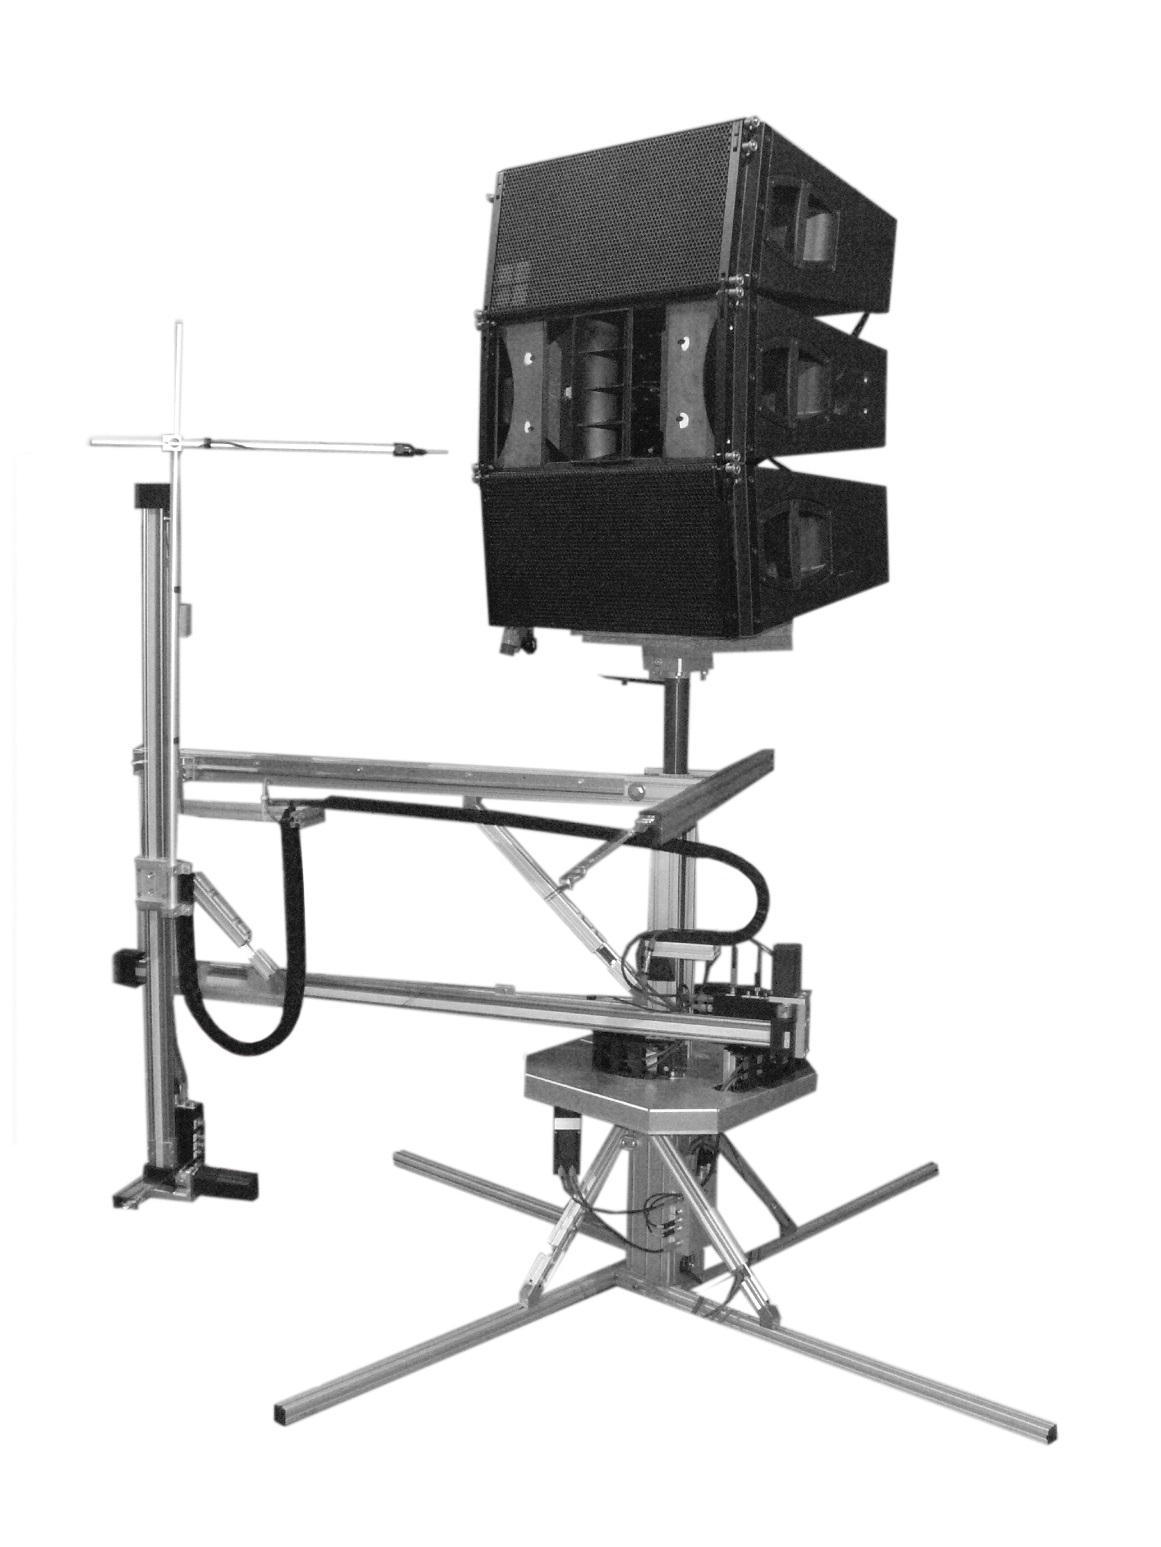
\includegraphics[scale=0.13]{Preface/NFS2} 
    \captionsetup{hypcap=false} 
	\captionof{figure}{Klippel Near Field Scanner} 
	\label{fig:nfs}
\end{center}
\end{minipage}\newline

This work has three main guidelines, which are the measurement of a speaker mounted on a baffle using the NFS and the enhancement of the measurement grid; the optimization of measurement time by exploiting symmetry conditions on the complex coefficients of the spherical wave expansion; and the application of room correction on non-anechoic measurements.\\

The NFS baffle measurement aims to create an application note on how to perform a near field scanning of a loudspeaker mounted on a baffle and evaluate the baffle's influence on the measurement. To do so, the required tasks are the assembly and critical evaluation a baffle prototype, and the optimization the measurement grid.\\
The measurement time optimization part aims to reduce the scanning effort of the NFS by assuming symmetry conditions on the DUT 's geometry and applying these conditions on the complex coefficients of the spherical wave expansion (see equation \ref{eq:sphwvexp}). \\
Finally, the room correction part aims to test and enhance the room correction module allowing to make fast non-anechoic measurements, to test a IEC standard tetrahedral measurement box provided by Geoff Hill \citep[see][]{tetbox}, and to create an application note on how to correct non-anechoic measurements, \\

There is no particular price constrains or technical constrains associated with this project, as the required hardware and software is already available. 

\newpage

	% LITERATURE REVIEW
\section{Literature review}

Performing measurements of a loudspeaker on a baffle can lead to many problems, mainly caused by the diffraction at the edges of the baffle, and the influence of the room on the measurement \cite{LIS}.\\
The Klippel Near Field Scanner uses the spherical wave expansion to determine the 3D sound pressure output of a DUT at any point in its far field, by performing a measurement in the nearfield of the DUT and solving the wave equation in spherical coordinates in order to apply the field separation method described by G. Weinreich and tested by M. Melon in the ASA publication \textit{Evaluation of a method for the measurement of subwoofers in usual rooms} and AES publication \textit{Comparison of four subwoofer measurement techniques}  \cite{melon1, melon2}. The complete theory behind this method is beyond the scope of this report, and will only be presented succinctly \citep[see][sect.~3]{aeshs} \citep[see][chap.~6]{Fourier}. 

\subsection{Field Separation}
\label{sec:FieldSep}

The solution of the three-dimensional wave equation in spherical coordinates can be described by a spherical wave expansion given by equation \ref{eq:sphwvexp} \cite{aeshs, train8}. The first expansion term, with the Hankel function of the second kind $h^{(2)}_{n}$, represents the outgoing waves; while the second expansion term, with the Hankel function of the first kind, represents the incoming waves. The Hankel functions contains the frequency dependence $e^{\pm j\omega t}$. The $Y_{n}^{m}(\theta, \phi)$ terms represents the spherical harmonics and describes the dependency on azimuthal angle $\phi$ and polar angle $\theta$. Finally, the terms $c_{n,m}^{out}(j \omega)$ and $c_{n,m}^{in}(j \omega)$ are weighting coefficients.


\begin{equation}
P(j\omega, r, \theta, \phi)  = \sum_{n=0}^{N}\sum_{m=-n}^{n}c_{mn}^{out}(j \omega)\cdot h_{n}^{(2)}(kr)\cdot Y_{n}^{m}(\theta, \phi)  + \sum_{n=0}^{N}\sum_{m=-n}^{n}c_{mn}^{in}(j \omega)\cdot h_{n}^{(1)}(kr)\cdot Y_{n}^{m}(\theta, \phi)
\label{eq:sphwvexp}
\end{equation}
\myequations{3D wave equation in spherical coordinates}

The free-field transfer function of a loudspeaker can be expressed by only considering the direct sound (outgoing wave) in equation \ref{eq:sphwvexp} and is expressed in equation \ref{eq:ffHf} \cite{aeswb}.

\begin{equation}
\begin{split}
H_{free}(f, \mathbf{r}) & = \sum_{N(f)}^{n=0}\sum_{n}^{m=-n}C_{mn}(f)\cdot h_{n}^{(2)}(kr)Y_{n}^{m}(\theta ,\phi )
\\ 
& = \mathbf{c}(f)\cdot \mathbf{b}(f,\mathbf{r})
\end{split}
\label{eq:ffHf}
\end{equation}
\myequations{Free-field transfer function of a loudspeaker in spherical coordinates}

Where $\mathbf{b}(f,\mathbf{r})$ represents the base functions used and are solution of the wave equation in spherical coordinates, and $\mathbf{c}(f)$ represents the weighting coefficients. \\
For non-anechoic measurements, an additional expansion term is required to describe the influence of external sound sources (room reflections, resonances) that are described by the Bessel function $j_{n}(kr)$, leading to the general solution for the sound field measured in a non-anechoic measurement given in equation \ref{eq:ffHt}  \cite{aeswb}.

\begin{equation}
\begin{split}
H_{test}(f, \mathbf{r}) &= \sum_{n=0}^{N(f)}\sum_{m=-n}^{n}\left [ C_{mn}(f)\cdot h_{n}^{(2)}(kr )\cdot Y_{n}^{m}(\theta ,\phi )+R_{mn}(f)\cdot j_{n}(kr)\cdot Y_{n}^{m}(\theta ,\phi ) \right ] \\
&= \mathbf{c}(f)\mathbf{b}(f,\mathbf{r})+\mathbf{r}(f)\mathbf{b}_{room}(f,\mathbf{r})
\end{split}
\label{eq:ffHt}
\end{equation}
\myequations{General solution for sound field measured in non-anechoic environments}

Where $\mathbf{c}(f)$ represents the outgoing coefficients and $\mathbf{r}(f)$ the incoming coefficients. \\
If the pressure is measured on 2 hemispherical surfaces in front of the baffle, the sound field can be expressed as equation \ref{eq:ffHt} for each surface. This can be expressed in matrix form by equation \ref{eq:holo_fieldsep} \cite{fieldsep}.

\begin{equation}
\begin{split}
&H_{1} = \mathbf{c}_{1}\mathbf{b}_{1}+\mathbf{r}_{1}\mathbf{b}_{room_{1}} \\
&H_{2} = \mathbf{c}_{2}\mathbf{b}_{2}+\mathbf{r}_{2}\mathbf{b}_{room_{2}}
\end{split}
\label{eq:holo_fieldsep}
\end{equation}
\myequations{System of equation of measured sound field}

Where the subscripts $1$ and $2$ refer to the two scanning surfaces. This system of equations can be assembled and expressed as equation \ref{eq:holo_matrix} \cite{fieldsep}.

\begin{equation}
H_{m} = M_{h}\mathbf{c}_{m}
\label{eq:holo_matrix}
\end{equation}
\myequations{Matrix form of measured sound field}

Where $ H_{m} $ represents the vector of measured pressures and $ \mathbf{c}_{m} $ the matrix of outgoing and outgoing coefficients. After retrieving the coefficient matrix $ \mathbf{c}_{m} $ by performing the inversion of equation \ref{eq:holo_matrix}, the outgoing field from the primary source can be retrieved and is expressed in equation \ref{eq:holo_solve}; where $A_{h}$ is the matrix containing the outgoing elementary waves $Y_{n}^{m}(\theta ,\phi )$ \cite{fieldsep}.

\begin{equation}
H_{out} = A_{h}\mathbf{c}_{out}
\label{eq:holo_solve}
\end{equation}
\myequations{Outgoing field solution for field separation}


Thanks to this field separation method, the speaker's SPL response can be isolated from any other components such as the effect of reflections on the room's walls, the diffraction at the edges of a system, or the acoustic shortcut between the rear and front sides of a baffle. \\
In high frequencies, where the ringing of loudspeaker is much shorter than the arrival time of the first room reflections; this method can be discarded and a time windowing applied on the Impulse Response of the system is sufficient to discriminate the outgoing and incoming waves \citep[see][sect.~3.1]{aeswb}. 



\subsection{Near Field measurements}

\subsubsection{Measurement principle}

The advantage of the Near Field compared to the Far Field measure is that the amplitude of the output is significantly higher in the Near Field, and the influence of the conditions (temperature, pressure) is minimized. \\
However, the Near-Field being much more complex than the Far Field, holographic processing is required to extrapolate the Far Field data. The complete process will be described succinctly, and can be found in details in the AES publication \textit{Holographic nearfield measurements of loudspeaker directivity} \cite{aeshs}.\\

\begin{center}
	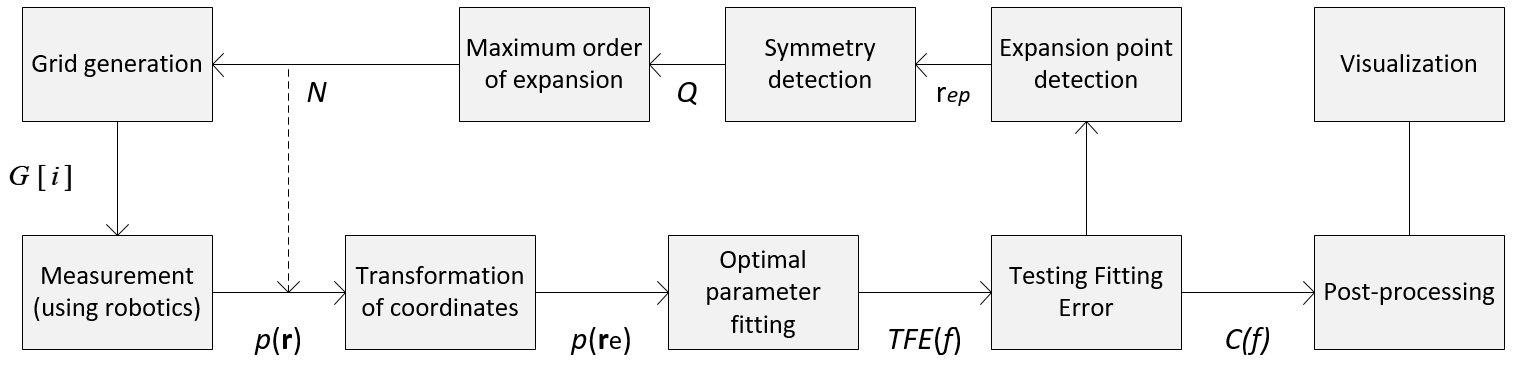
\includegraphics[width=0.8\textwidth]{Preface/NFS_Flowchart} 
    \captionsetup{hypcap=false} 
	\captionof{figure}{NFS measurement principle flowchart} 
	\label{fig:nfsflow}
\end{center}

Figure \ref{fig:nfsflow} presents a flowchart of the measurement principle. \\ 
The first step of the scanning process is the generation of the measurement grid. The main difficulty is to avoid spacial aliasing, which is achieved by generating a non-uniform grid. Once the grid is generated, the measurement is conducted thanks to the robotics.\\
The measurement being done, the first step of the holographic process is to shift the coordinates of all measurements points to fit the expansion point $r_{E}$ of the system, by using equation \ref{eq:coordtrans}. The expansion point is the center of the spherical waves from equation \ref{eq:sphwvexp}, and its position might change with frequency. This step is required for further processing, in order to make sure that the calculated Far Field is relevant.
\begin{equation}
\mathbf{r}_{E}(f) = \mathbf{Q}(f)\mathbf{r}+\mathbf{r}_{EP}(f)-\mathbf{r}_{ref}
\label{eq:coordtrans}
\end{equation}
\myequations{Coordinates transformation}

Then, the parameters are fitted to find the optimum coefficients $C_{mn}$. This is done by estimating the deviation $e(f,r_{E})$ between the measured and the modeled transfer function of the system, as expressed in equation \ref{eq:ParamFit}. 

\begin{equation}
\mathbf{c}(f)= \textup{arg} \; \textup{min}\left ( \sum_{\forall \mathbf{r}_{e}\in G}\left | e(f,\mathbf{r}_{e}) \right | ^{2} \right )
\label{eq:ParamFit}
\end{equation}
\myequations{Parameter fitting}

The accuracy of the holographic estimation of the sound field is then verified by estimating the Total Fitting Error ($TFE$) of the measurement. This parameter is calculated from the ratio of the truncated of the power series at a maximum order $N$ of the deviation $e(f,r_{E})$ by the transfer function of the system. Evaluating the $TFE$ allows to verify the accuracy of a measurement: if it is lower than -20 dB, it is considered that the holographic model describes the Far-Field of the system with sufficient accuracy. 

\begin{equation}
TFE(f) = 10\textup{log}\left ( \frac{\sum_{\mathbf{r}_{e}\in G}\left | e(f,\mathbf{r}_{e}) \right |^{2}}{\sum_{\mathbf{r}_{e}\in G}\left | H(f,\mathbf{r}_{e}) \right |^{2}} \right )
\label{eq:TFE}
\end{equation}
\myequations{Total Fitting Error}

Another verification is the estimation of the Multi-Layer Error (MLE), given by equation \ref{eq:MLE}. This parameter allows to check the agreement between the error at the points $ \mathbf{r}_{e} $ on the outer layer and the error at the closest points $ \mathbf{r}'_{e} $ on the inner layer. 

\begin{equation}
MLE = 10log\left ( \frac{\sum_{\mathbf{r}_{e}\in G}\left | e(f,\mathbf{r}_{e})-e\textup{'}(f,\mathbf{r}\textup{'}_{e}) \right |^{2}}{\sum_{\mathbf{r}_{e}\in G} \left |H(f,\mathbf{r}_{e})  \right |^{2}-\left |H\textup{'}(f,\mathbf{r}\textup{'}_{e})  \right |^{2} } \right )
\label{eq:MLE}
\end{equation}
\myequations{Multi Layer Error}

Comparing the $ TFE $ and the $MLE$ allows to estimate the measurement's relevancy: if the errors have the same order of magnitude, it is considered that the measurement is polluted.

\subsubsection{Maximum order of expansion}

The maximum order of expansion $N$ is a very important parameter to obtain accurate data. The higher it is and the more accurate the model becomes, but the longer the calculation. In that regard, a trade-off between accuracy and calculation time has to be made. \\

Investigations on this parameter have already been conducted \cite{pres, aeshs, train8} and have shown that a wave expansion truncated after $N$ = 10 is capable of modeling the 3D sound pressure field of a DUT above 30 Hz with sufficient accuracy. \\
\todo[inline]{Développer les limites fréquencielles du systeme}

At very low frequencies the measurement is polluted by the poor Signal to Noise Ratio (SNR) between the microphone's input and the noise; and increasing the maximum order of expansion has little to no effect on the $TFE$. 


%--------------------------------------------------------------
%	BAFFLE MEASUREMENT
%--------------------------------------------------------------
\chapter{Baffle measurements}

\section{Grid optimization}

\subsection{Principle}
\begin{minipage}{0.6\textwidth}
For baffle measurements, the only possible scanning grid was a spherical grid, that might not be optimized for all types of drivers. A solution to this problem would be to implement different types of grids that the user could switch between in order to have a better agreement with the DUT's geometry. \\
The first grid that have been implemented is an elliptical grid. To do so, the spherical grid is generated using the existing code, and projected onto an elliptical surface of minor and major radius defined by the user, as shown in figure \ref{fig:el_grid}. \\~\\
\end{minipage}
\begin{minipage}{0.4\textwidth}
\begin{center}
	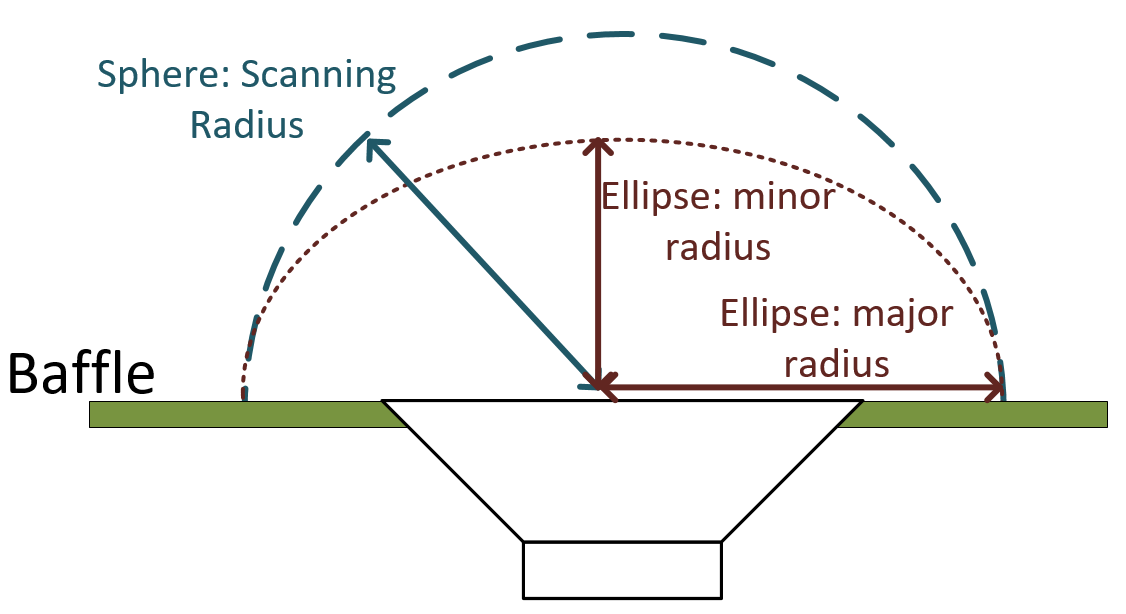
\includegraphics[scale=0.21]{GridOpti/El_Grid_Draw} 
    \captionsetup{hypcap=false} 
	\captionof{figure}{Elliptical grid} 
	\label{fig:el_grid}
\end{center}
\end{minipage}

The projection to an elliptical grid have been implemented by using the following calculations: first of all, the equation of a line $y = f(x)$ intercepting y-axis in zero gives the slope $m = \frac{y}{x}$. Introducing in the ellipse equation and using $y = m*x$ leads to a solution for x, given by equation \ref{eq:ellipse}, where $a$ is the major radius and $b$ the minor radius.

\begin{equation}
\left ( \frac{x}{a} \right )^{2} + \left ( \frac{y}{b} \right )^{2} = 1 \; \; \;  \Leftrightarrow \; \; \;  x = \sqrt{\frac{a^{2}b^{2}}{b^{2}+a^{2}m}}
\label{eq:ellipse}
\end{equation}
\myequations{Ellipse equation and solution for x}

The values of y-coordinates can then by calculated from the slope by using $y = mx$. 

\subsection{Measurements}

After implementation of the elliptical grid projection in Scilab, a 10 cm woofer (see \ref{spkrlib:10cm}) have been measured using the NFS. The scan was performed using a spherical grid with a scanning radius of 30 cm, and an elliptical grid with a major radius of 30 cm and a minor radius of 10 cm. Both measurements have been done in the same conditions: equal input voltage, same number of points, and same position of the DUT. The results are presented in figures \ref{fig:comp_ElSPh_SPL} and \ref{fig:comp_ElSPh_Pow}. \\

\begin{minipage}{0.5\textwidth}
\begin{center}
	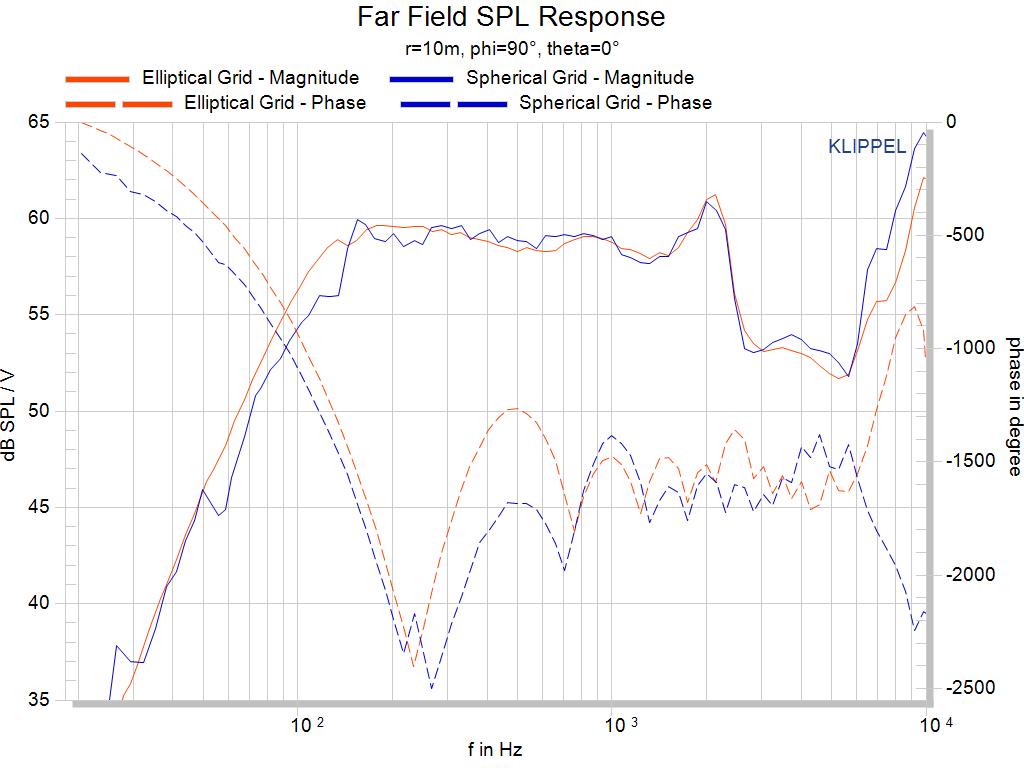
\includegraphics[width=.9\textwidth]{GridOpti/FF_Compa_El_Sph}
    \captionsetup{hypcap=false} 
	\captionof{figure}{Far Field SPL response} 
	\label{fig:comp_ElSPh_SPL}
\end{center}
\end{minipage}
\begin{minipage}{0.5\textwidth}
\begin{center}
	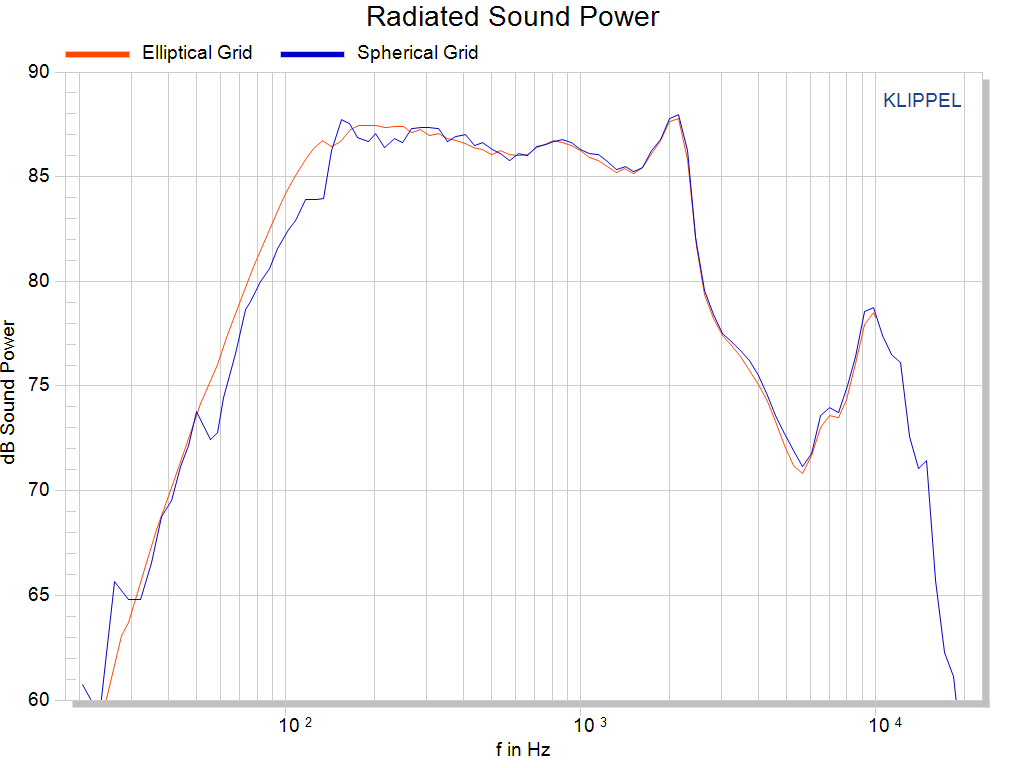
\includegraphics[width=.9\textwidth]{GridOpti/SP_Compa_El_Sph}
    \captionsetup{hypcap=false} 
	\captionof{figure}{Radiated Sound Power} 
	\label{fig:comp_ElSPh_Pow}
\end{center}
\end{minipage}
\vspace{0.1cm}

\subsection{Discussion}

Observing the magnitude of the Far Field SPL response, it can be noted that the elliptical grid provides a much smoother curve than the spherical grid, especially in the low frequencies. This effect could be explained by the fact that the measurement points being much closer to the driver, it is much less sensible to systematic errors that cannot be removed by Field Separation, such as the baffle vibrating inside the scanning radius. \\

The phase of the Far Field SPL Response gives interesting results. The elliptical grid's phase presents less phase shifts, meaning that less resonances are present on this measurement, matching with the previous hypothesis of a removed systematic error due to the baffle vibrating. \\

The radiated sound Power is extremely similar for both measurements, which was expected considering that the same speaker have been measured twice using in equal configuration. Similarly to the Far Field SPL response, the curve is smoothed when using an elliptical grid. \\

It can be concluded that using different measurement grid is relevant. A well adjusted grid have shown to give more accurate results. Following this investigation, several grids could be generated, for example a half-cylindrical grid for rectangular systems mounted in baffle, such as wall speakers.\\
Further investigations should be conducted on the influence of the measurement grid on the measurement accuracy.

% \subsection{Application note for baffle measurements}
\todo[inline]{make reference to application note for baffle measurements}
% Another task was to create an application note to explain how to perform baffle measurements to Klippel's customers. This document being quite heavy, it is given in appendix \ref{chap:AN_Baffle}.

\section{Estimation of baffle influence}

\subsection{Presentation of the prototype}

\begin{minipage}{0.6\textwidth}
A baffle prototype has been designed to allow relevant measurements of devices mounted on a baffle with the NFS. The prototype is shown figure \ref{fig:baffle_proto}. More pictures are given in appendix \textbf{MAKE REFERENCE}. \\

Before starting the production of this item, a critical evaluation must be performed in order to estimate the influence of the baffle on the measurement. Different analysis will be conduced, mainly to check the vibration of the baffle itself, the vibration of the wood plate used to mount the speaker, and a measurement centered on the speaker in order to have a point of comparison to identify vibration problems.
\end{minipage}
\begin{minipage}{0.4\textwidth}
\begin{center}
	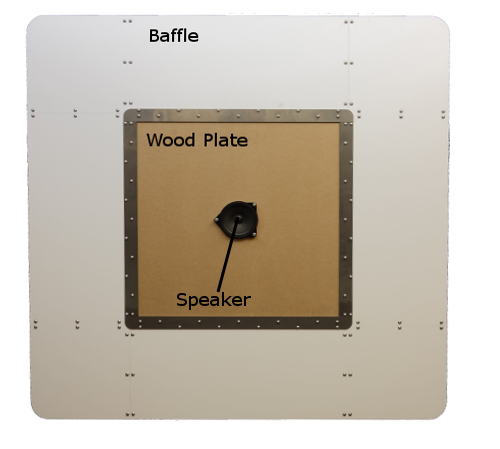
\includegraphics[width=0.8\textwidth]{GridOpti/Baffle_Alone_2} 
    \captionsetup{hypcap=false} 
	\captionof{figure}{Baffle Prototype} 
	\label{fig:baffle_proto}
\end{center}
\end{minipage} 

\subsection{Measurements}

Figure \ref{fig:vib_pow} present the apparent power in the near field of the DUT for different measurements points. \\
The blue curve represents the power from the speaker. This scan have been centered on the speaker, using a 5 cm radius for the scanning grid. The bright orange curve represents the contribution form the speaker and the wooden plate: this scan was centered on the speaker, with a 21 cm radius for the scanning grid. The grey curve represents the contribution from the baffle: the scan was centered on the lower right corner of the baffle, with a 5 cm scanning radius. Finally, the light orange curve represents the contribution from the wooden plate: this scan was centered midway between the speaker and the baffle, with a 5 cm scanning radius. \\

Comparing the contributions from the speaker with the speaker + wood allows to estimate how the wooden plate vibration impacts the system: the differences between the 2 plots can only come from the plate vibration, as the field separation method removed all contributions from the room. \\
Comparing the variations on the speaker+wood results with the contribution of the wood shows that most of the variations matches with the peaks of the wood's contribution; whereas s few variations matches with the baffle contribution's peaks (see figure \ref{Curves:Baffle_RadPow} for matching peaks and a bigger figure). \\

Moreover, the contributions from the baffle itself aren't really problematic: if the scanning radius is correctly chosen, the field separation method will remove the baffle's contribution from the measurement. The contributions from the wooden plate are much more problematic, since the field separation method cannot remove contributions coming from inside the scanning radius, and the scanning radius cannot be smaller than the driver's. 

\begin{minipage}{0.5\textwidth} % Figures
\begin{center}
	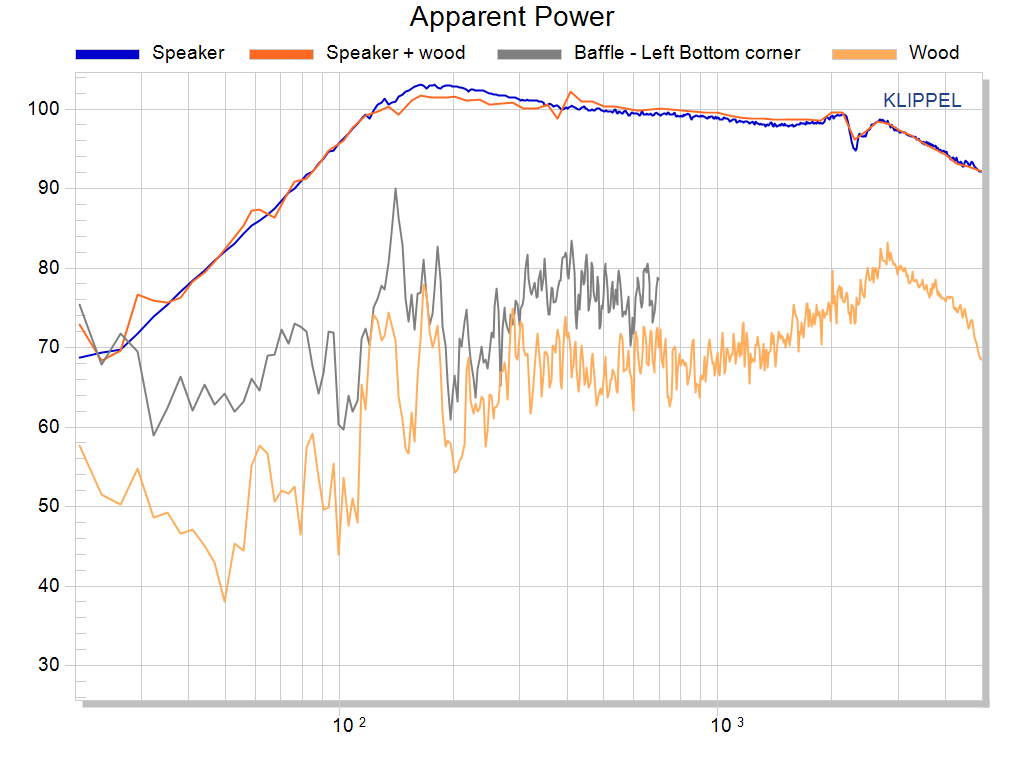
\includegraphics[width=\textwidth]{GridOpti/Vib_Pow} 
\end{center}
    \captionsetup{hypcap=false} 
	\captionof{figure}{Comparison of apparent power in the Near Field for different measurement points} 
	\label{fig:vib_pow}
\end{minipage}
\begin{minipage}{0.5\textwidth}
\begin{center}
	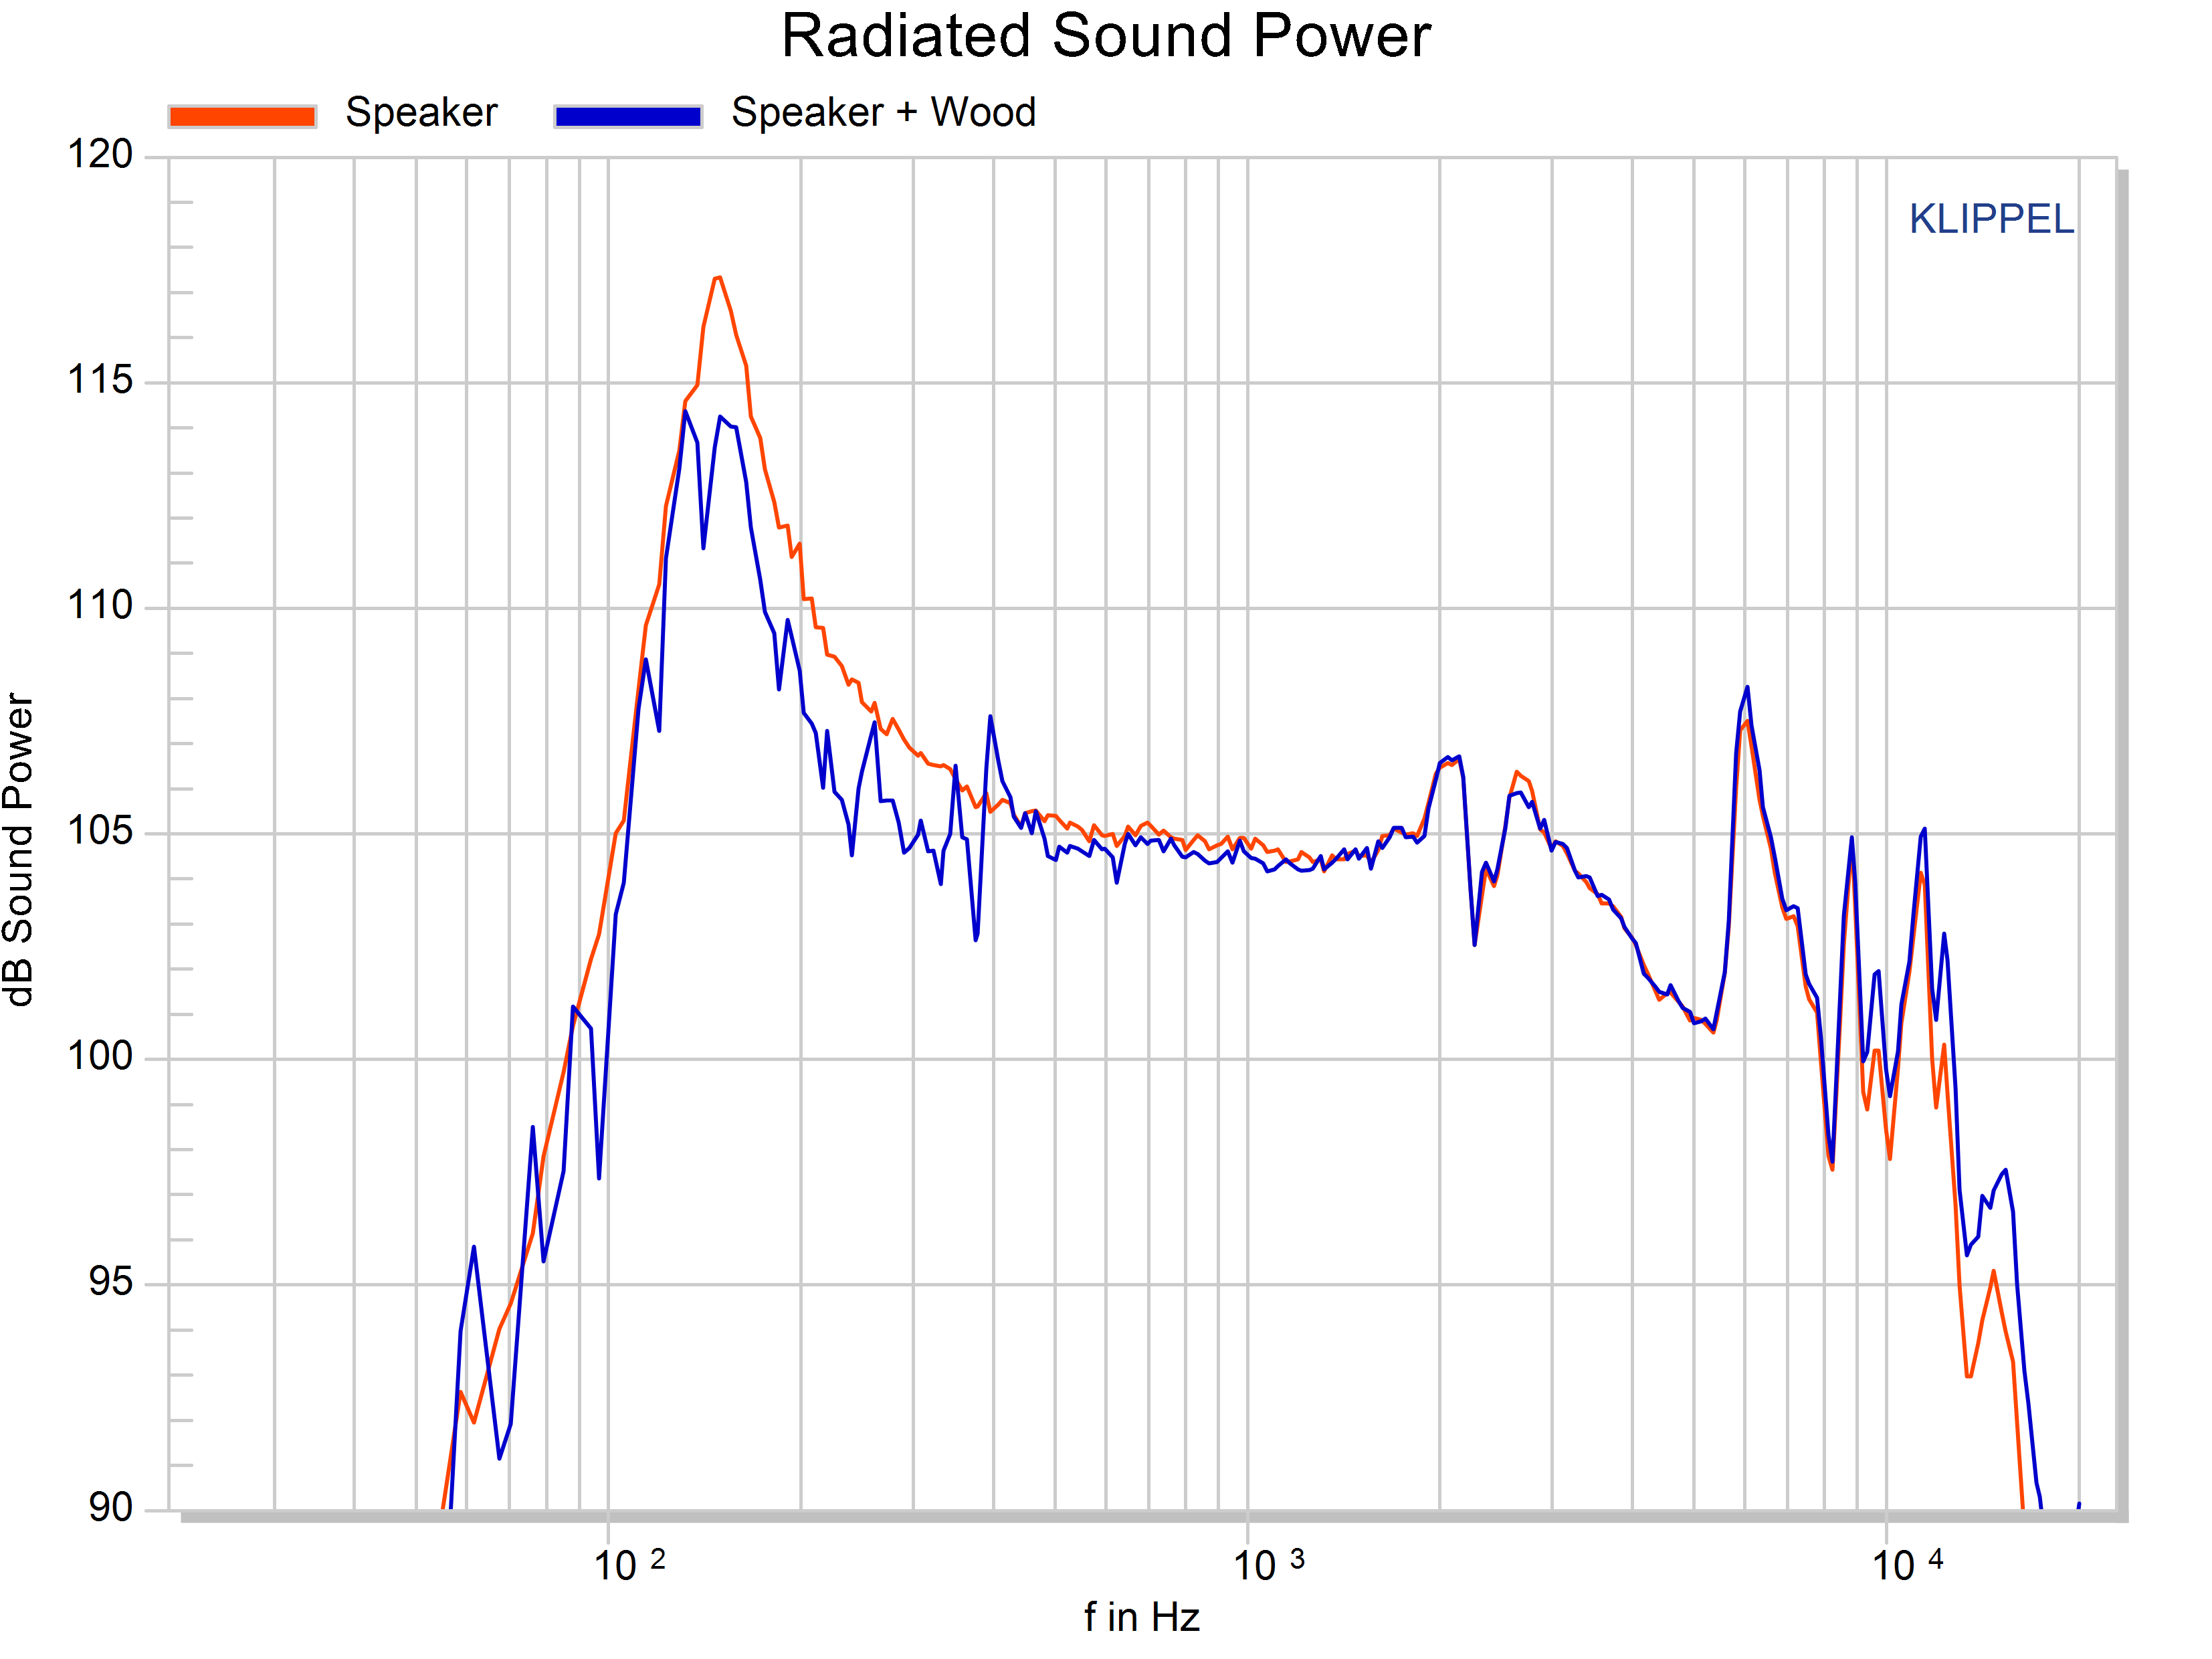
\includegraphics[width=\textwidth]{GridOpti/Vib_Pow_SPW} 
\end{center}
    \captionsetup{hypcap=false} 
	\captionof{figure}{Comparison of radiated powers in the Far Field for the speaker and speaker + wood measurements} 
	\label{fig:vib_comp}
\end{minipage}
\vspace{0.1cm}

Figure \ref{fig:vib_comp} compares the radiated powers in the far field (r = 10m) of the speaker and the speaker+wood measurements, evidencing the effect of the wooden plate's vibration on the measurement. At the resonance (f = 150 Hz), a strong cancellation effect is observed on the speaker+wood measurement, with a difference of almost 6dB between the curves. This cancellation is most likely to be due to the plate vibrating in opposite phase with the speaker. \\
The movie bellow shows an animation\footnote{If the animation is not playing correctly, \href{https://www.dropbox.com/sh/1jlodpb3biuxmhy/AADFRz8B249n8ERu3nkwyyisa?dl=0}{please download it by clicking \underline{here}.}} of a scan performed on the baffle using Klippel's laser scanning system, at f = 190 Hz. The plate is vibrating in opposite phase with the speaker,  which confirms the previous hypothesis of the wooden plate creating a cancellation effect on the Sound Pressure response of the driver. 

\ifdraft
\begin{center}
	\includemovie[draft,repeat,poster,label=baffle_vib,text={\small(Click to start...)}]{6cm}{4cm}{GridOpti/baffle_vib.avi}
\end{center}
\else
\begin{center}
	\includemovie[repeat,poster,label=baffle_vib,text={\small(Click to start...)}]{6cm}{4cm}{GridOpti/baffle_vib.avi}
\end{center}
\fi


\subsection{Discussion}

The previous investigations highlighted several problems with the baffle prototype. Particular attention should be given to the following:
\begin{description}
\item[Wooden plate] special attention should be given to its thickness, material and damping. A solution to attenuate the vibration of the plate would be to stiffen it by attaching beams to the backside. As a general advice, MDF should be avoided because of its lightness. 
\item[Clamping system] the system clamping the plate in place is not satisfying to conduct acoustical measurements. The nuts supposed to hold the wooden plate in place are subject to rattling, even when strongly tightened.
\item[Baffle] the baffle itself generates some vibration, that is believed to not be critical for the measurements since it can be removed by using the field identification. Maybe damping could be added, although the baffle cannot be modified too much. 
\end{description}


%--------------------------------------------------------------
%	SYMMETRY
%--------------------------------------------------------------

\chapter{Measurement time optimization}

\section{Principle}

Exploiting symmetry conditions on the complex coefficients of the spherical wave expansion $c_{n,m}^{out}(j \omega)$ (see equation \ref{eq:sphwvexp}) could reduce the measurement time significantly by reducing the number of points of the measurement as explained in the article \textit{Holographic Nearfield Measurement of Loudspeaker Directivity} \citep[][sect.~4]{aeshs}. \\

To implement this, the idea is to start from a measurement done with a coarse grid, and to check the existence of symmetry condition on the coefficients by using the different equations provided in appendix \ref{chap:sym}. The symmetries under study are given in appendix \ref{chap:sym}.
Once the coefficients satisfying each symmetry condition have been found, the symmetry factor (given by equations \ref{eq:Srs}, \ref{eq:Sdps}, \ref{eq:Sbs}, \ref{eq:Ssps}) is estimated. By setting different thresholds, the user is informed that the DUT may present certain types of symmetry that could be used to perform a faster full measurement.

\begin{center}
	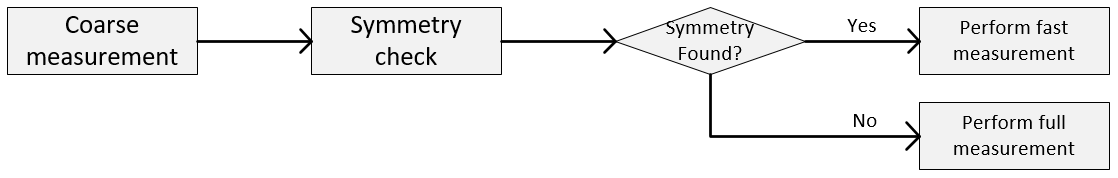
\includegraphics[width=0.7\textwidth]{Sym/flowchart} 
    \captionsetup{hypcap=false} 
	\captionof{figure}{Flowchart of the symmetry check} 
	\label{fig:sym_flow}
\end{center}

\section{Measurements}

After implementation in SciLab, the validity of the symmetry assumptions must be verified. To do so, different measurements have been performed of several speakers presenting interesting geometries. A library of these speakers is given in appendix \ref{chap:spk_lib}. 

\todo[inline, color=red!40]{Rephrase... ca sonne pas très bien je trouve}

\subsection{10 cm woofer}

The DUT is a circular, 10 cm woofer (see appendix \ref{spkrlib:10cm}), mounted on the baffle. \\

\begin{minipage}{0.5\textwidth}
\begin{center}
	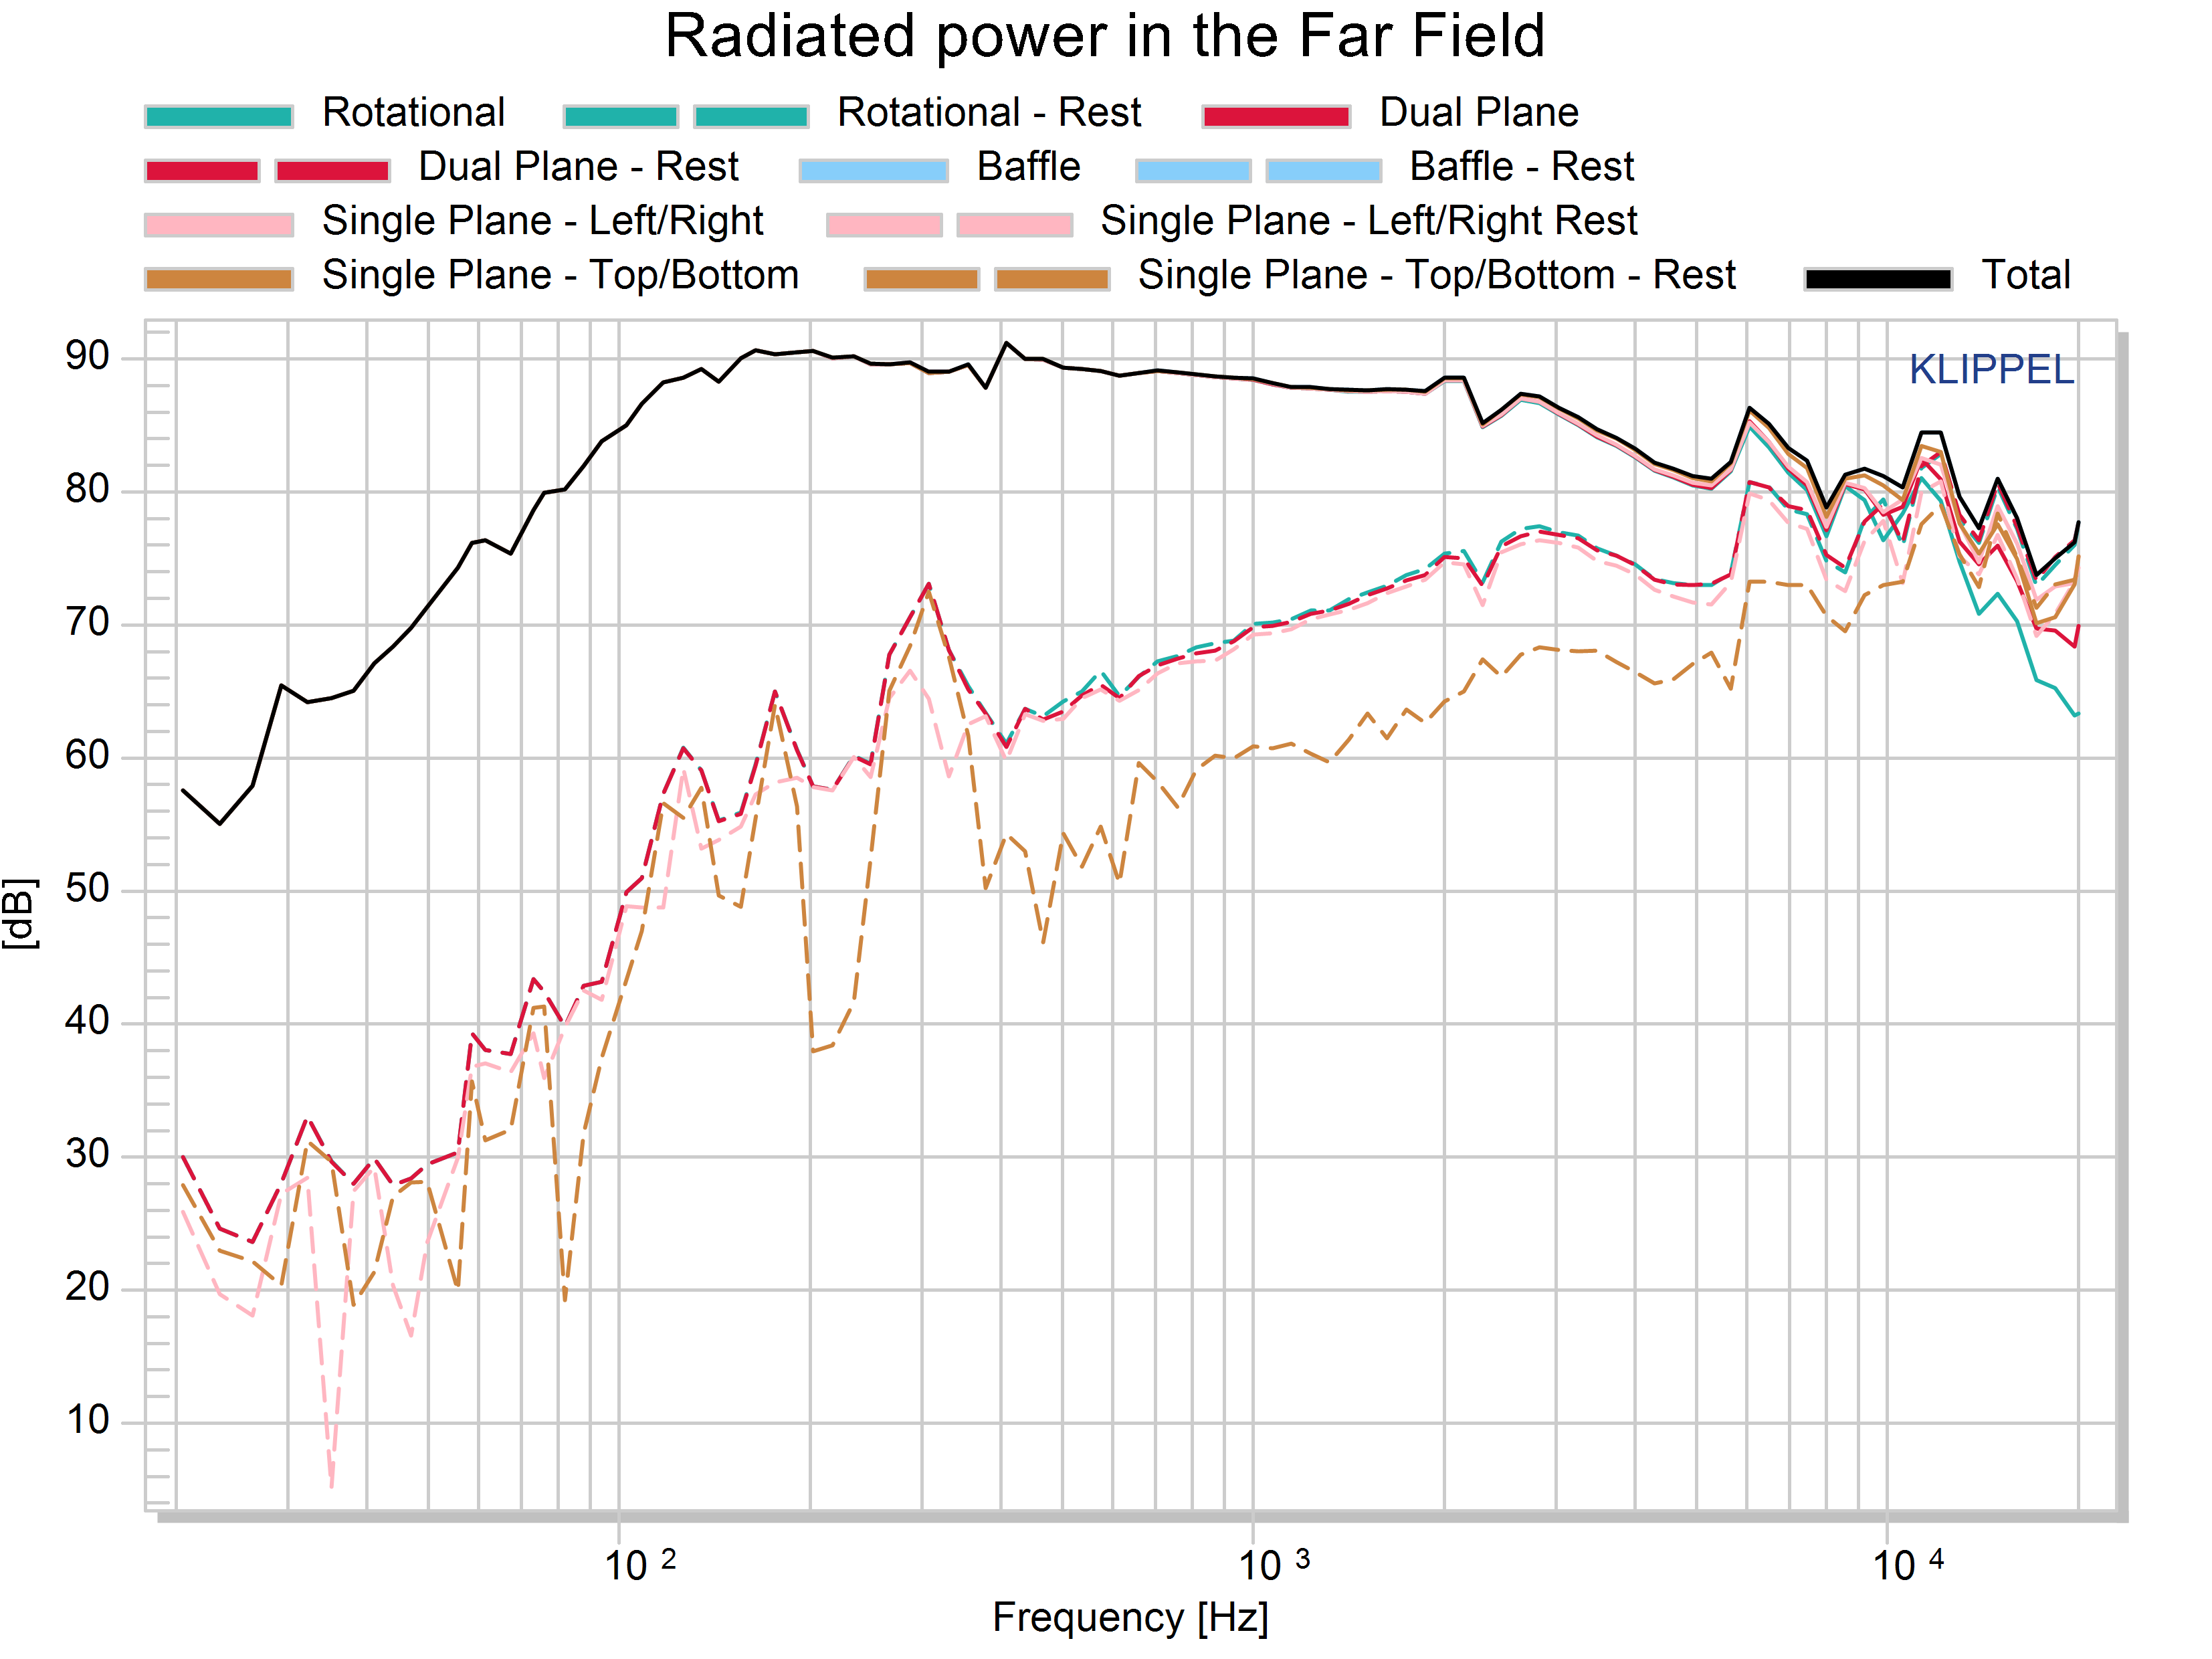
\includegraphics[width=\textwidth]{Sym/Rad_Pow_10cmWoofer} 
    \captionsetup{hypcap=false} 
	\captionof{figure}{Radiated Powers of 10cm woofer} 
	\label{fig:rad_pow_10cm}
\end{center}
\end{minipage}
\begin{minipage}{0.5\textwidth}
\begin{center}
	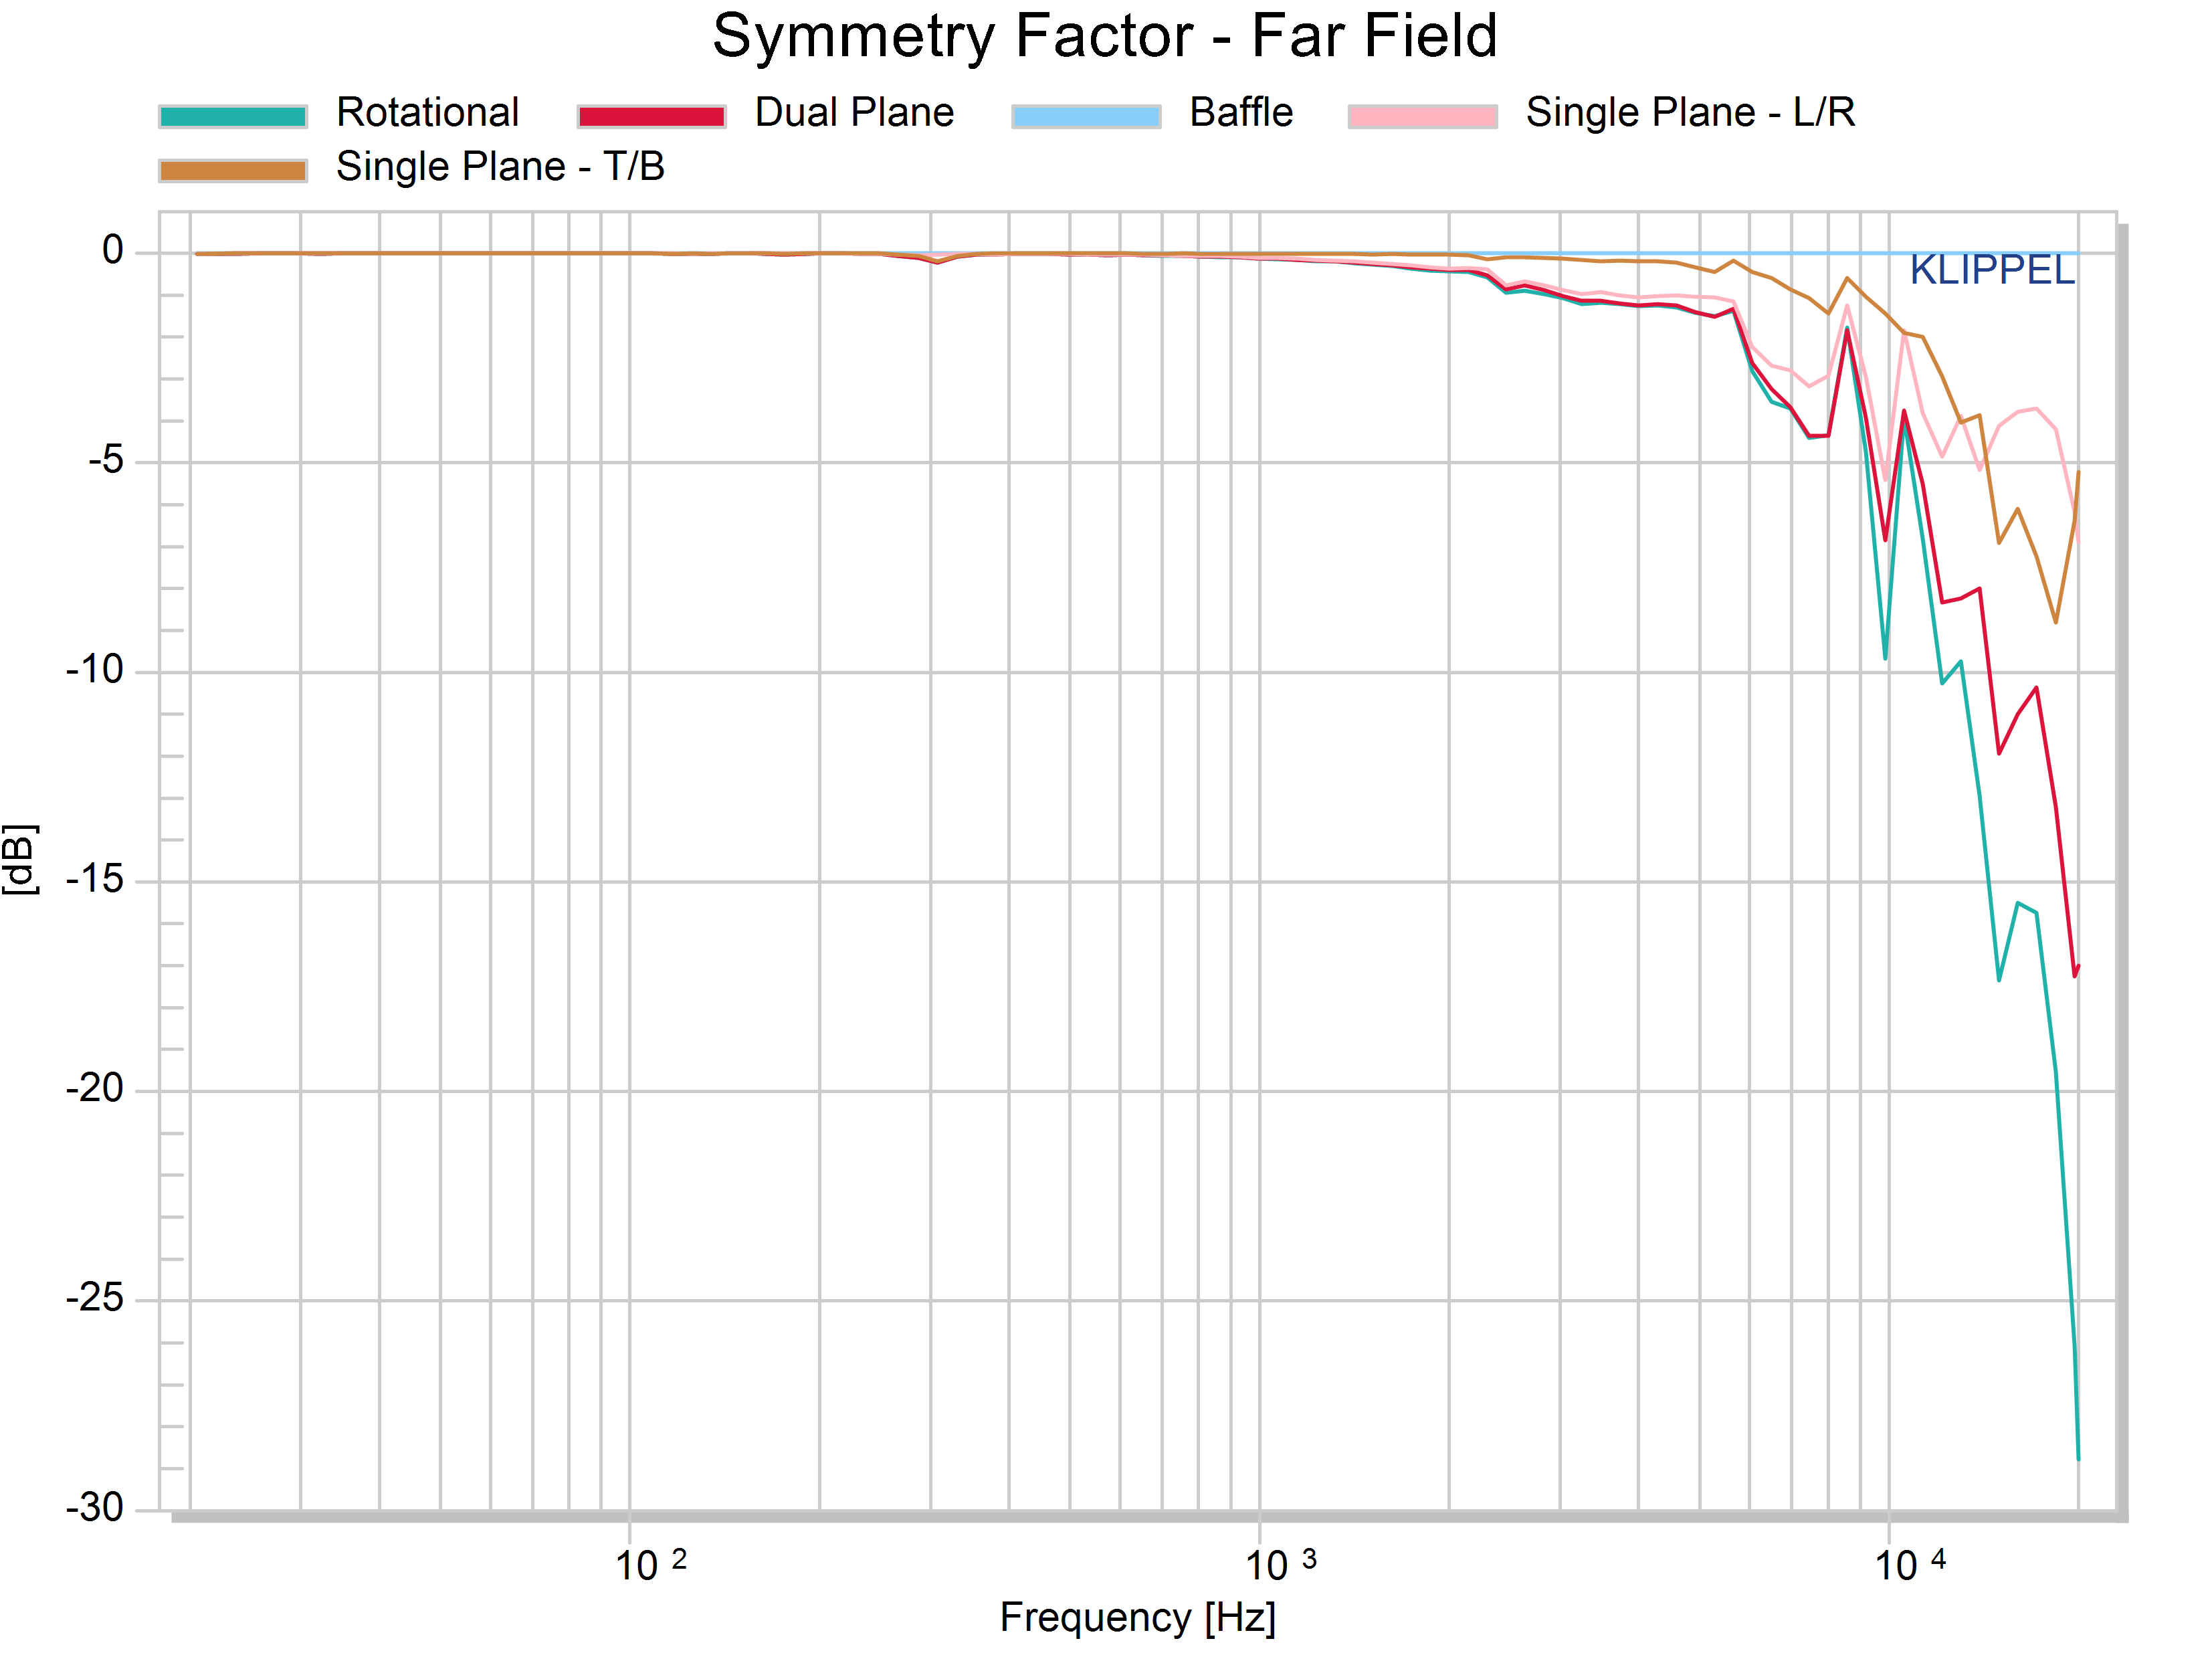
\includegraphics[width=\textwidth]{Sym/Sym_Fact_10cmWoofer} 
    \captionsetup{hypcap=false} 
	\captionof{figure}{Symmetry Factors of 10cm woofer} 
	\label{fig:sym_fact_10cm}
\end{center}
\end{minipage}
\vspace{0.1cm}

Figure \ref{fig:rad_pow_10cm} presents the calculated radiated powers for different symmetry conditions. The dashed curves represents the "rest", which is the radiated power by coefficients not satisfying the symmetry condition described in appendix \ref{chap:sym}, in the example of a rotational symmetry the rest will be all coefficients $C_{mn} \neq 0 \;  \textup{for m}  \neq 0$. For a better reading, all the radiated power curves are provided in separate graphs in appendix \ref{Curves:10cm}.\\

Figure \ref{fig:sym_fact_10cm} presents the symmetry factors for different types of symmetry, expressed in dB. A 0 dB value means that the power radiated by considering only the coefficients satisfying the symmetry condition and the total radiated power present no differences. Observing the symmetry factor for the baffle symmetry shows that this value is 0 dB over the whole frequency band: this result is matching the expectations since the measurement have been done with the speaker mounted on a baffle. \\

Comparing the radiated power in figure \ref{fig:rad_pow_10cm} and appendix \ref{Curves:10cm} for the different symmetries gives interesting results: in the low frequency domain, the total radiated power and the powers radiated by the different symmetry conditions presents no differences, no matter the symmetry type. In low frequency, the driver behaves as a monopole and have an omnidirectional directivity pattern; fulfilling all the symmetry conditions. \\
However, in high frequencies, disruptions appears and the rest increases significantly: the higher the frequency, and the more interferences will be produced by the speaker. This can be observed on the contour plot of the woofer's directivity, presented in appendix \ref{fig:contour_10cm}. \\

Comparing the symmetry factors shows that the most present symmetries are the Single Plane symmetries. This result may be unexpected and one could expect the rotational symmetry to be dominant, but as seen with the radiated powers in high frequencies the speaker isn't a monopole: the cone breakups spoils the rotational symmetry. 

\subsection{Oval speaker}
The DUT is an oval speaker (see appendix \ref{spkrlib:oval}), mounted on the baffle. The particular geometry of this speaker gives hints about the expected results: the rotational symmetry should be the lowest one, and the planar symmetries should be dominant (single plane or dual plane symmetries).  Figures \ref{fig:rad_pow_Oval} and \ref{fig:sym_fact_Oval} presents the radiated powers and the symmetry factors respectively. The radiated powers are presented in separated graphs in appendix \ref{Curves:oval}.\\

\begin{minipage}{0.5\textwidth}
\begin{center}
	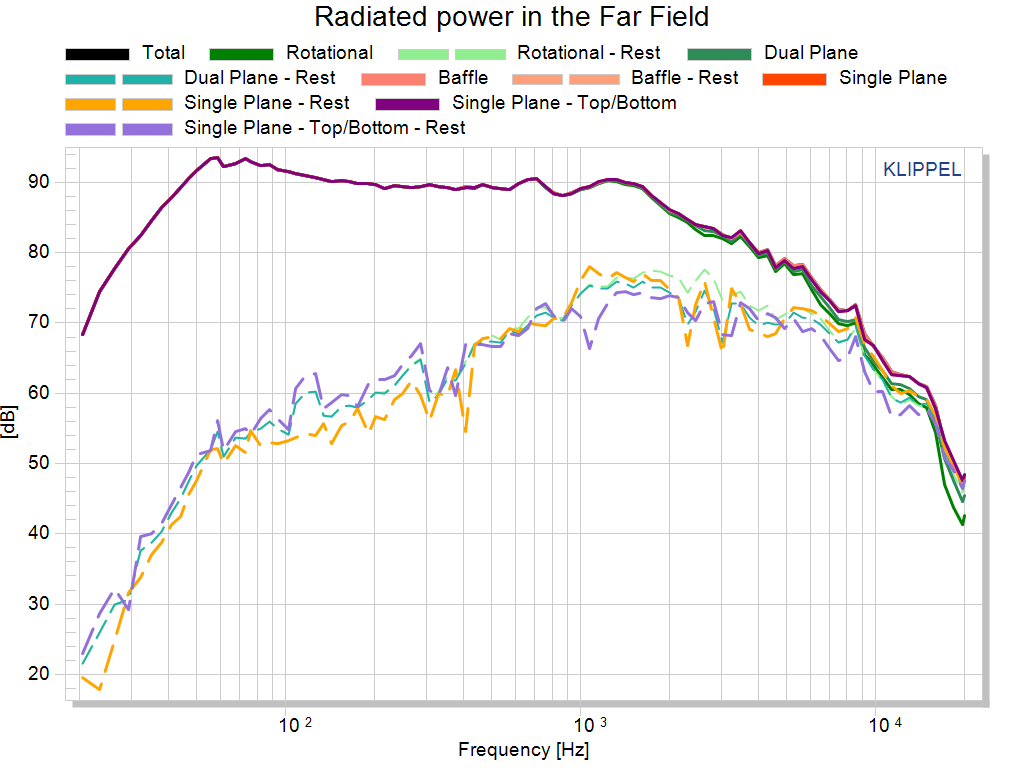
\includegraphics[width=\textwidth]{Sym/Rad_Pow_OvalSpkr} 
    \captionsetup{hypcap=false} 
	\captionof{figure}{Radiated Powers of oval speaker} 
	\label{fig:rad_pow_Oval}
\end{center}
\end{minipage}
\begin{minipage}{0.5\textwidth}
\begin{center}
	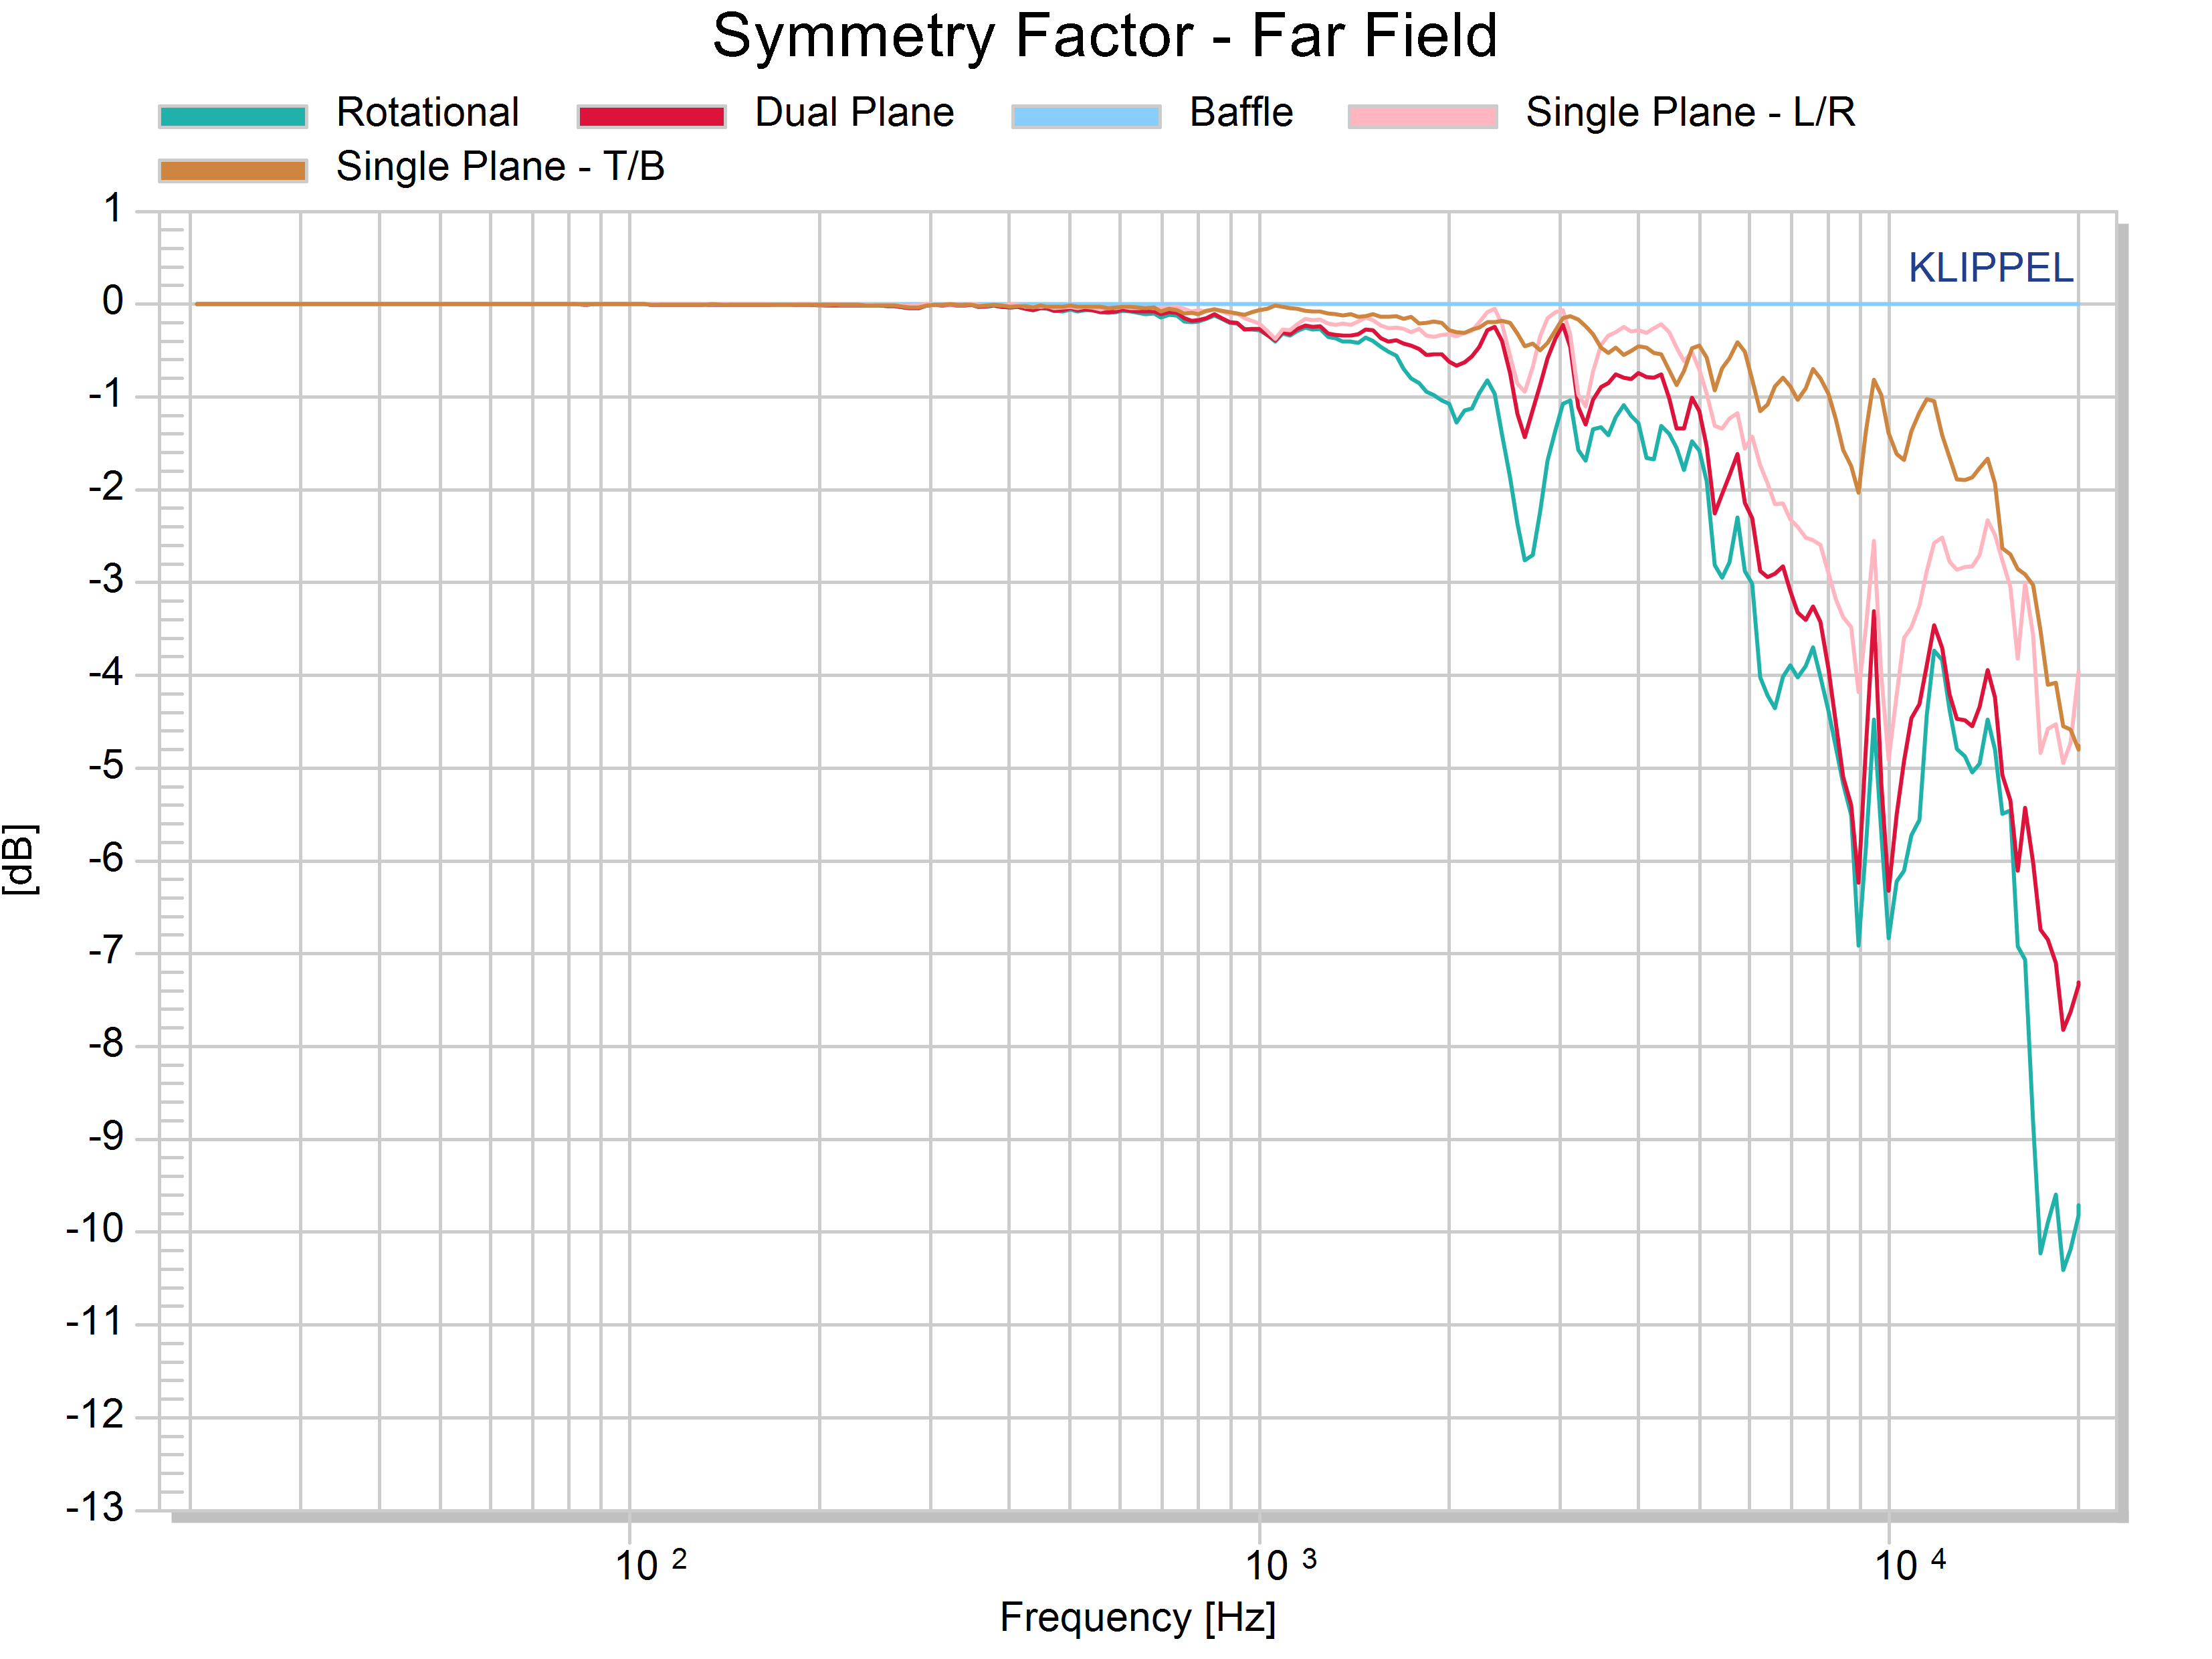
\includegraphics[width=\textwidth]{Sym/Sym_Fact_OvalSpkr} 
    \captionsetup{hypcap=false} 
	\captionof{figure}{Symmetry Factors of oval speaker} 
	\label{fig:sym_fact_Oval}
\end{center}
\end{minipage}
\vspace{0.1cm}

Observing the radiated powers for the different symmetries, it is found that in the 20 Hz - 1.5 kHz range there is no differences between the total radiated power and the symmetries radiated power. Similarly to the 10 cm woofer, the drivers behaves as a monopole in this range. This is observed on the contour plot provided in figure \ref{Curves:oval_contour}. \\
After 1.5 kHz, differences appear for the Dual Plane, Single Plane and Rotational symmetries. Characterizing the speaker's behavior in higher frequencies requires to look at the symmetry factors. However, it can already be observed that the power radiated by rotational symmetry coefficients is bellow all other radiated powers after 1.5 kHz, meaning that the rotational symmetry condition is not satisfied. \\

Observing the symmetry factors shows that the rotational symmetry factor is below all other factors, matching with the expected behavior of the driver. The baffle symmetry factor is 0 dB over the whole frequency range, as expected for a measure performed with a driver mounted on baffle.

\begin{minipage}{0.5\textwidth}
Interestingly, the top/bottom single plane symmetry factor is higher than other symmetry factors from 5 kHz. This could be explained by the speaker's geometry: the larger dimension makes it more prone to rocking mode, spoiling the left/right single plane symmetry. At 9400 Hz there is a peak on the symmetry factors and the radiated power, probably due to a membrane mode.\\

Figure \ref{fig:phase_Oval} the phase balloon at this frequency shows that the left and right side of the membrane vibrates with in opposite phase, validating the hypothesis of the left/right symmetry condition not being satisfied because of the rocking modes of the driver's membrane. 
\end{minipage}
\begin{minipage}{0.5\textwidth}
\begin{center}
	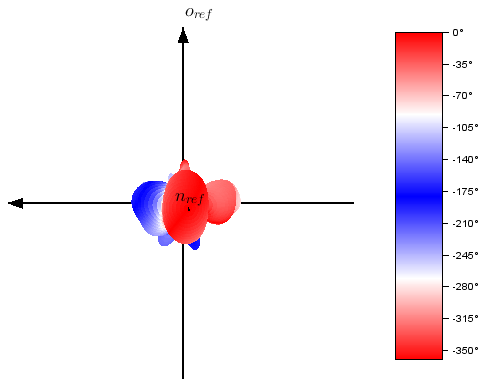
\includegraphics[width=0.8\textwidth]{Sym/phase_oval} 
    \captionsetup{hypcap=false} 
	\captionof{figure}{Phase balloon at f = 9400 Hz of oval speaker} 
	\label{fig:phase_Oval}
\end{center}
\end{minipage}

\subsection{2-way "diagonal" speaker}

The DUT is a "diagonal" 2-way speaker, and the scan is centered on the tweeter (see appendix \ref{spkrlib:BnO}). This speaker's asymmetrical geometry is very interesting for the symmetry measurement. The device also have an integrated crossover. Figures \ref{fig:rad_pow_BnO} and \ref{fig:sym_fact_BnO} presents the radiated powers and the symmetry factors respectively. The radiated powers are plotted in separated graphs in appendix \ref{Curves:2way}. \\

\begin{minipage}{0.5\textwidth}
\begin{center}
	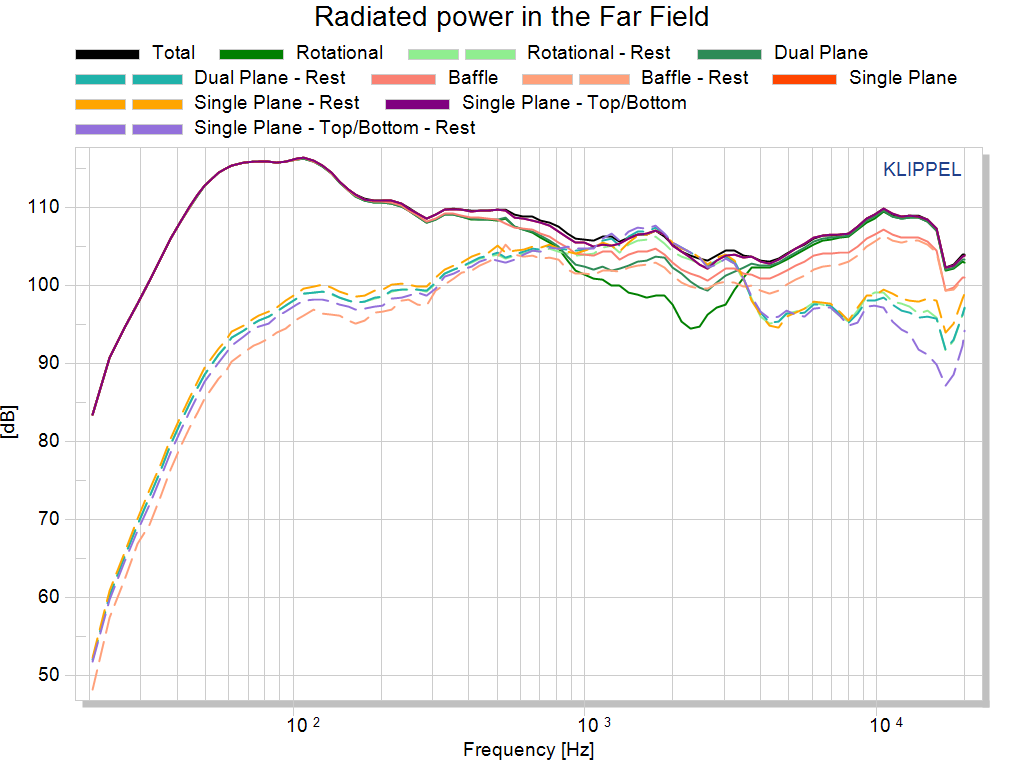
\includegraphics[width=\textwidth]{Sym/Rad_Pow_BnO} 
    \captionsetup{hypcap=false} 
	\captionof{figure}{Radiated Powers of diagonal speaker} 
	\label{fig:rad_pow_BnO}
\end{center}
\end{minipage}
\begin{minipage}{0.5\textwidth}
\begin{center}
	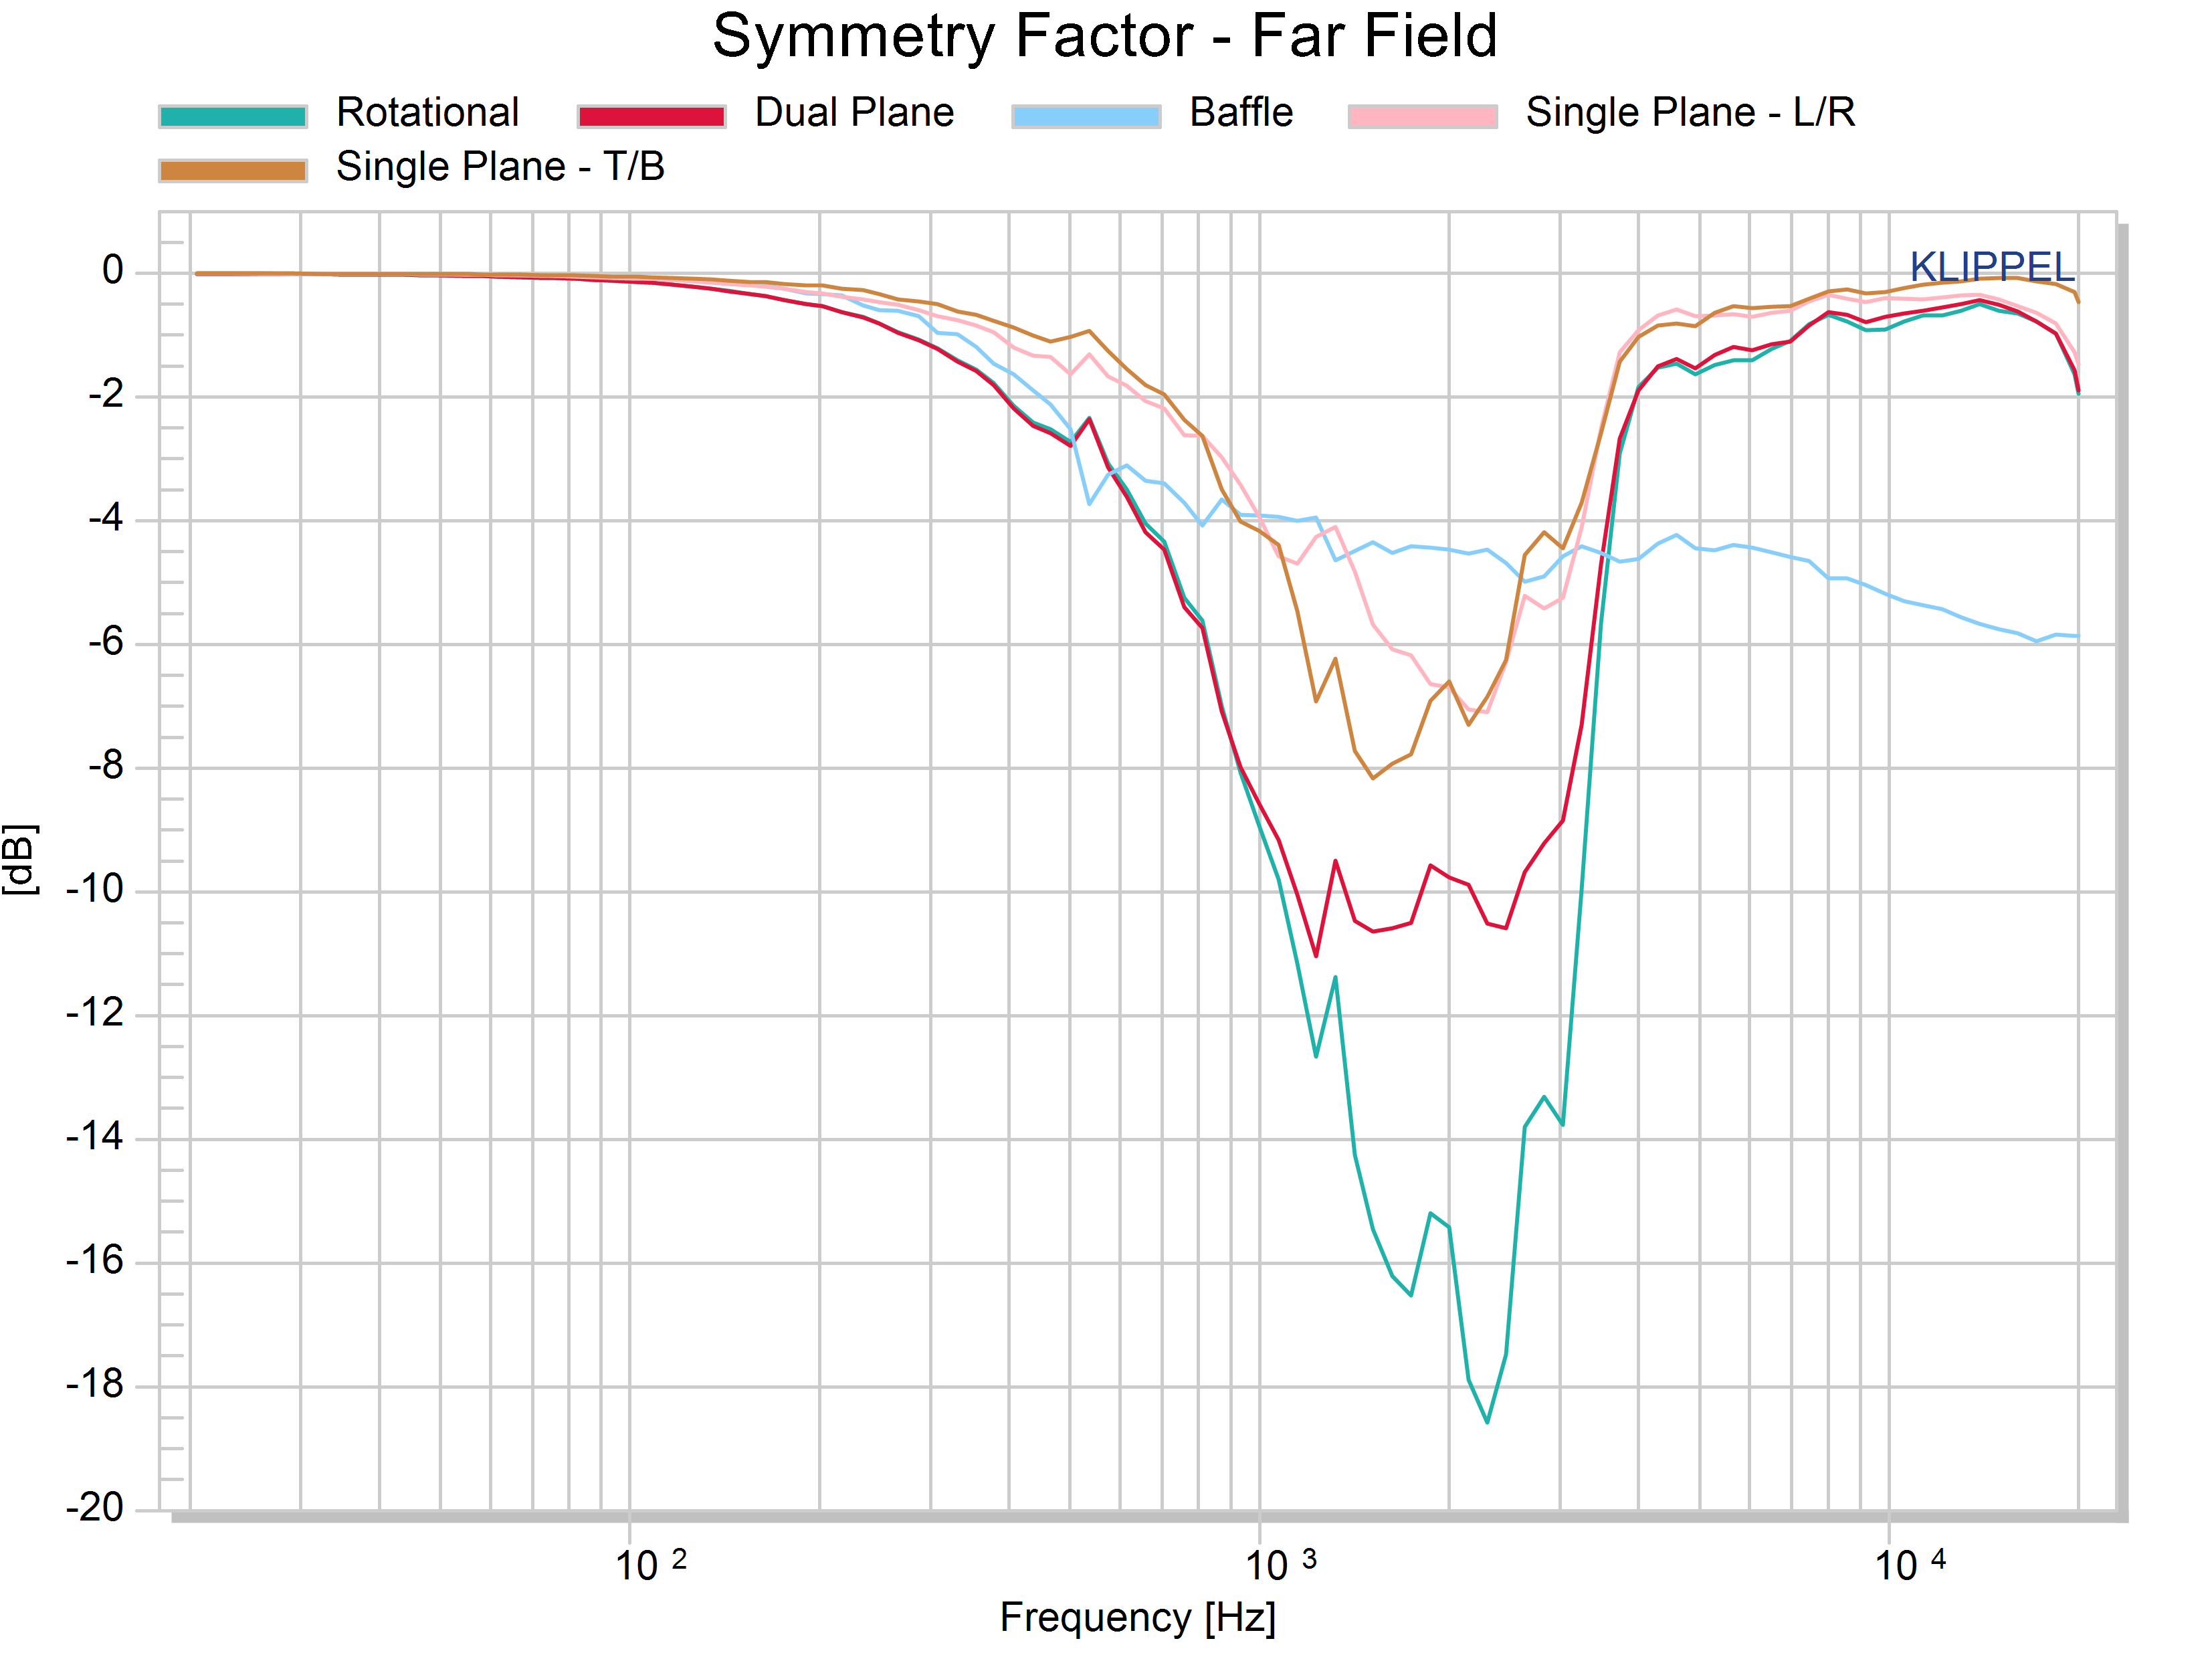
\includegraphics[width=\textwidth]{Sym/Sym_Fact_BnO} 
    \captionsetup{hypcap=false} 
	\captionof{figure}{Symmetry Factors of diagonal speaker} 
	\label{fig:sym_fact_BnO}
\end{center}
\end{minipage}

\vspace{0.1cm}

Observing the radiated powers shows that the systems have an omnidirectional behavior until 175 Hz, shown by the contour plot in figure \ref{Curves:2way_contour}. Unlike the previous measurements, this system have 2 drivers emitting, making it less susceptible to present symmetries.\\
The crossover frequency range can be observed clearly on both result result curves: the symmetry factors take a dip, and the rest powers are higher than the symmetrical powers. \\

Observing the Symmetry Factors shows that there is no baffle symmetry for this measurement. Although this result might seem quite trivial since the DUT was not mounted on a baffle, it is good indication that the symmetry estimation works correctly. Another interesting observation is at the crossover frequency: the symmetry factors take a dip. \\
In this frequency range, both drivers of the DUT are working, and due to their positioning there is no possible symmetry condition. In low frequency, the driver is a monopole, so all symmetry conditions are fulfilled.\\

In high frequency when the twitter alone is emitting, some symmetry is observed. The Top/Bottom single plane symmetry have the highest coefficients, meaning that it could be possible to measure only the top half of this driver and to deduce the coefficients using equation \ref{eq:spsym}.\\



\subsection{Studio Monitor}
 The DUT is a 2-way studio monitor (see appendix \ref{sprklib:Studio}). Similarly to the 2-way diagonal speaker, this system have a built-in crossover. Figures \ref{fig:rad_pow_studio} and \ref{fig:sym_fact_studio} presents the radiated powers and the symmetry factors respectively.
\todo[inline, color=red!40]{Make appendix in spkr lib, add figures, and explain them}

\begin{minipage}{0.5\textwidth}
\begin{center}
	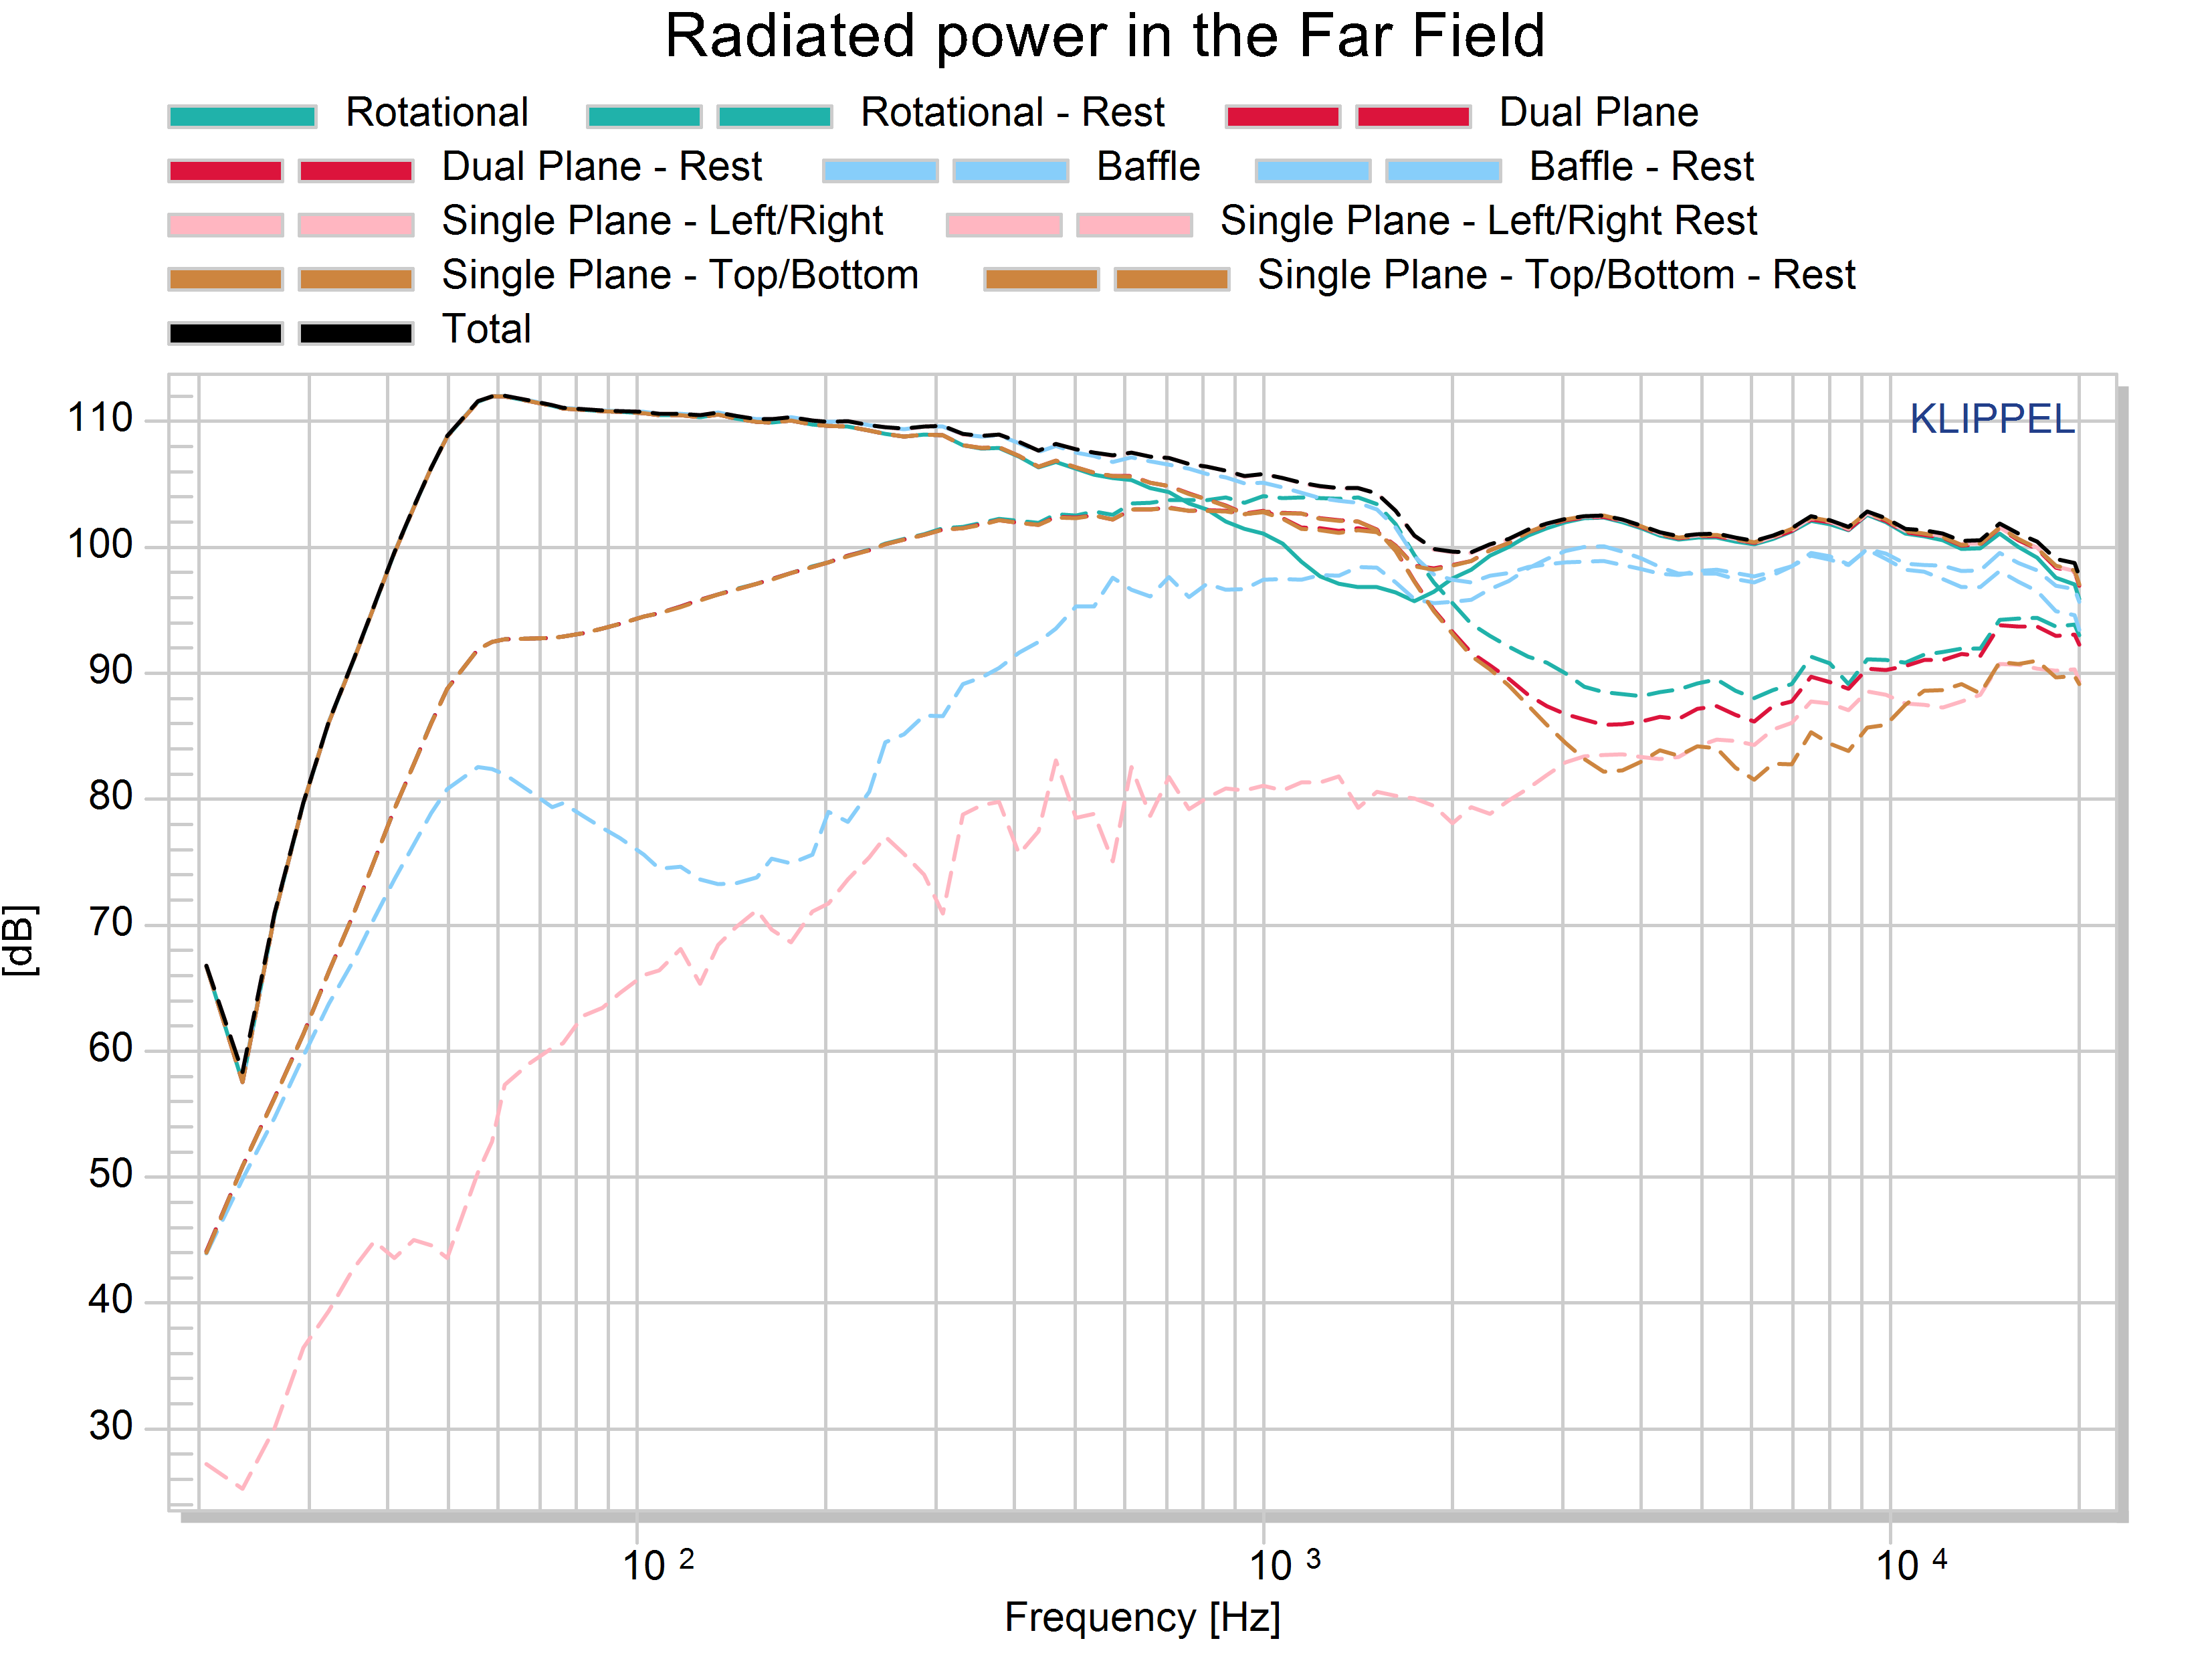
\includegraphics[width=\textwidth]{Sym/Rad_Pow_studio} 
    \captionsetup{hypcap=false} 
	\captionof{figure}{Radiated Powers of studio monitor} 
	\label{fig:rad_pow_studio}
\end{center}
\end{minipage}
\begin{minipage}{0.5\textwidth}
\begin{center}
	\includegraphics[width=\textwidth]{Sym/Sym_Fact_studio} 
    \captionsetup{hypcap=false} 
	\captionof{figure}{Symmetry Factors of studio monitor} 
	\label{fig:sym_fact_studio}
\end{center}
\end{minipage}
\vspace{0.1cm}

\section{Discussion}

The previous results are promising for the investigation on symmetry conditions to ease off the measurement time. The calculated symmetry factors match with the expected results for all measurements, and can be implemented in the NFS scripts to be exploited for reducing the number of measurements points. 

\todo[inline, color=red!40]{Finish the discussion and see how your code have been implemented}

%--------------------------------------------------------------
%	ROOM CORRECTION
%--------------------------------------------------------------
\chapter{Room correction}

\section{Principle}

Being able to generate room correction curves is great for the everyday measurement of loudspeakers since it allows to compensate the effect of any environment and to create quasi-perfect measurements. According to the AES standard \cite{aesstandart}, "\textit{accurate and repeatable loudspeaker driver measurements require that environmental and boundary influence have minimal impact on the measurement}". Such measurements are usually done in anechoic rooms, and accurate results are difficult to achieve for companies not having access to such a room or for a hobbyist. \\

A solution to this problematic is to measure in test boxes, such as the tetrahedral test box created by Hill Acoustics \citep[see][]{tetbox}. By using post-processing, it is possible to generate a correction curve for the box, and to obtain accurate measurements by compensating its influence on the DUT. Several methods are available to generate this room correction curves \citep[see][]{aeswb}.\\

\begin{minipage}{0.33\textwidth}
\begin{center}
	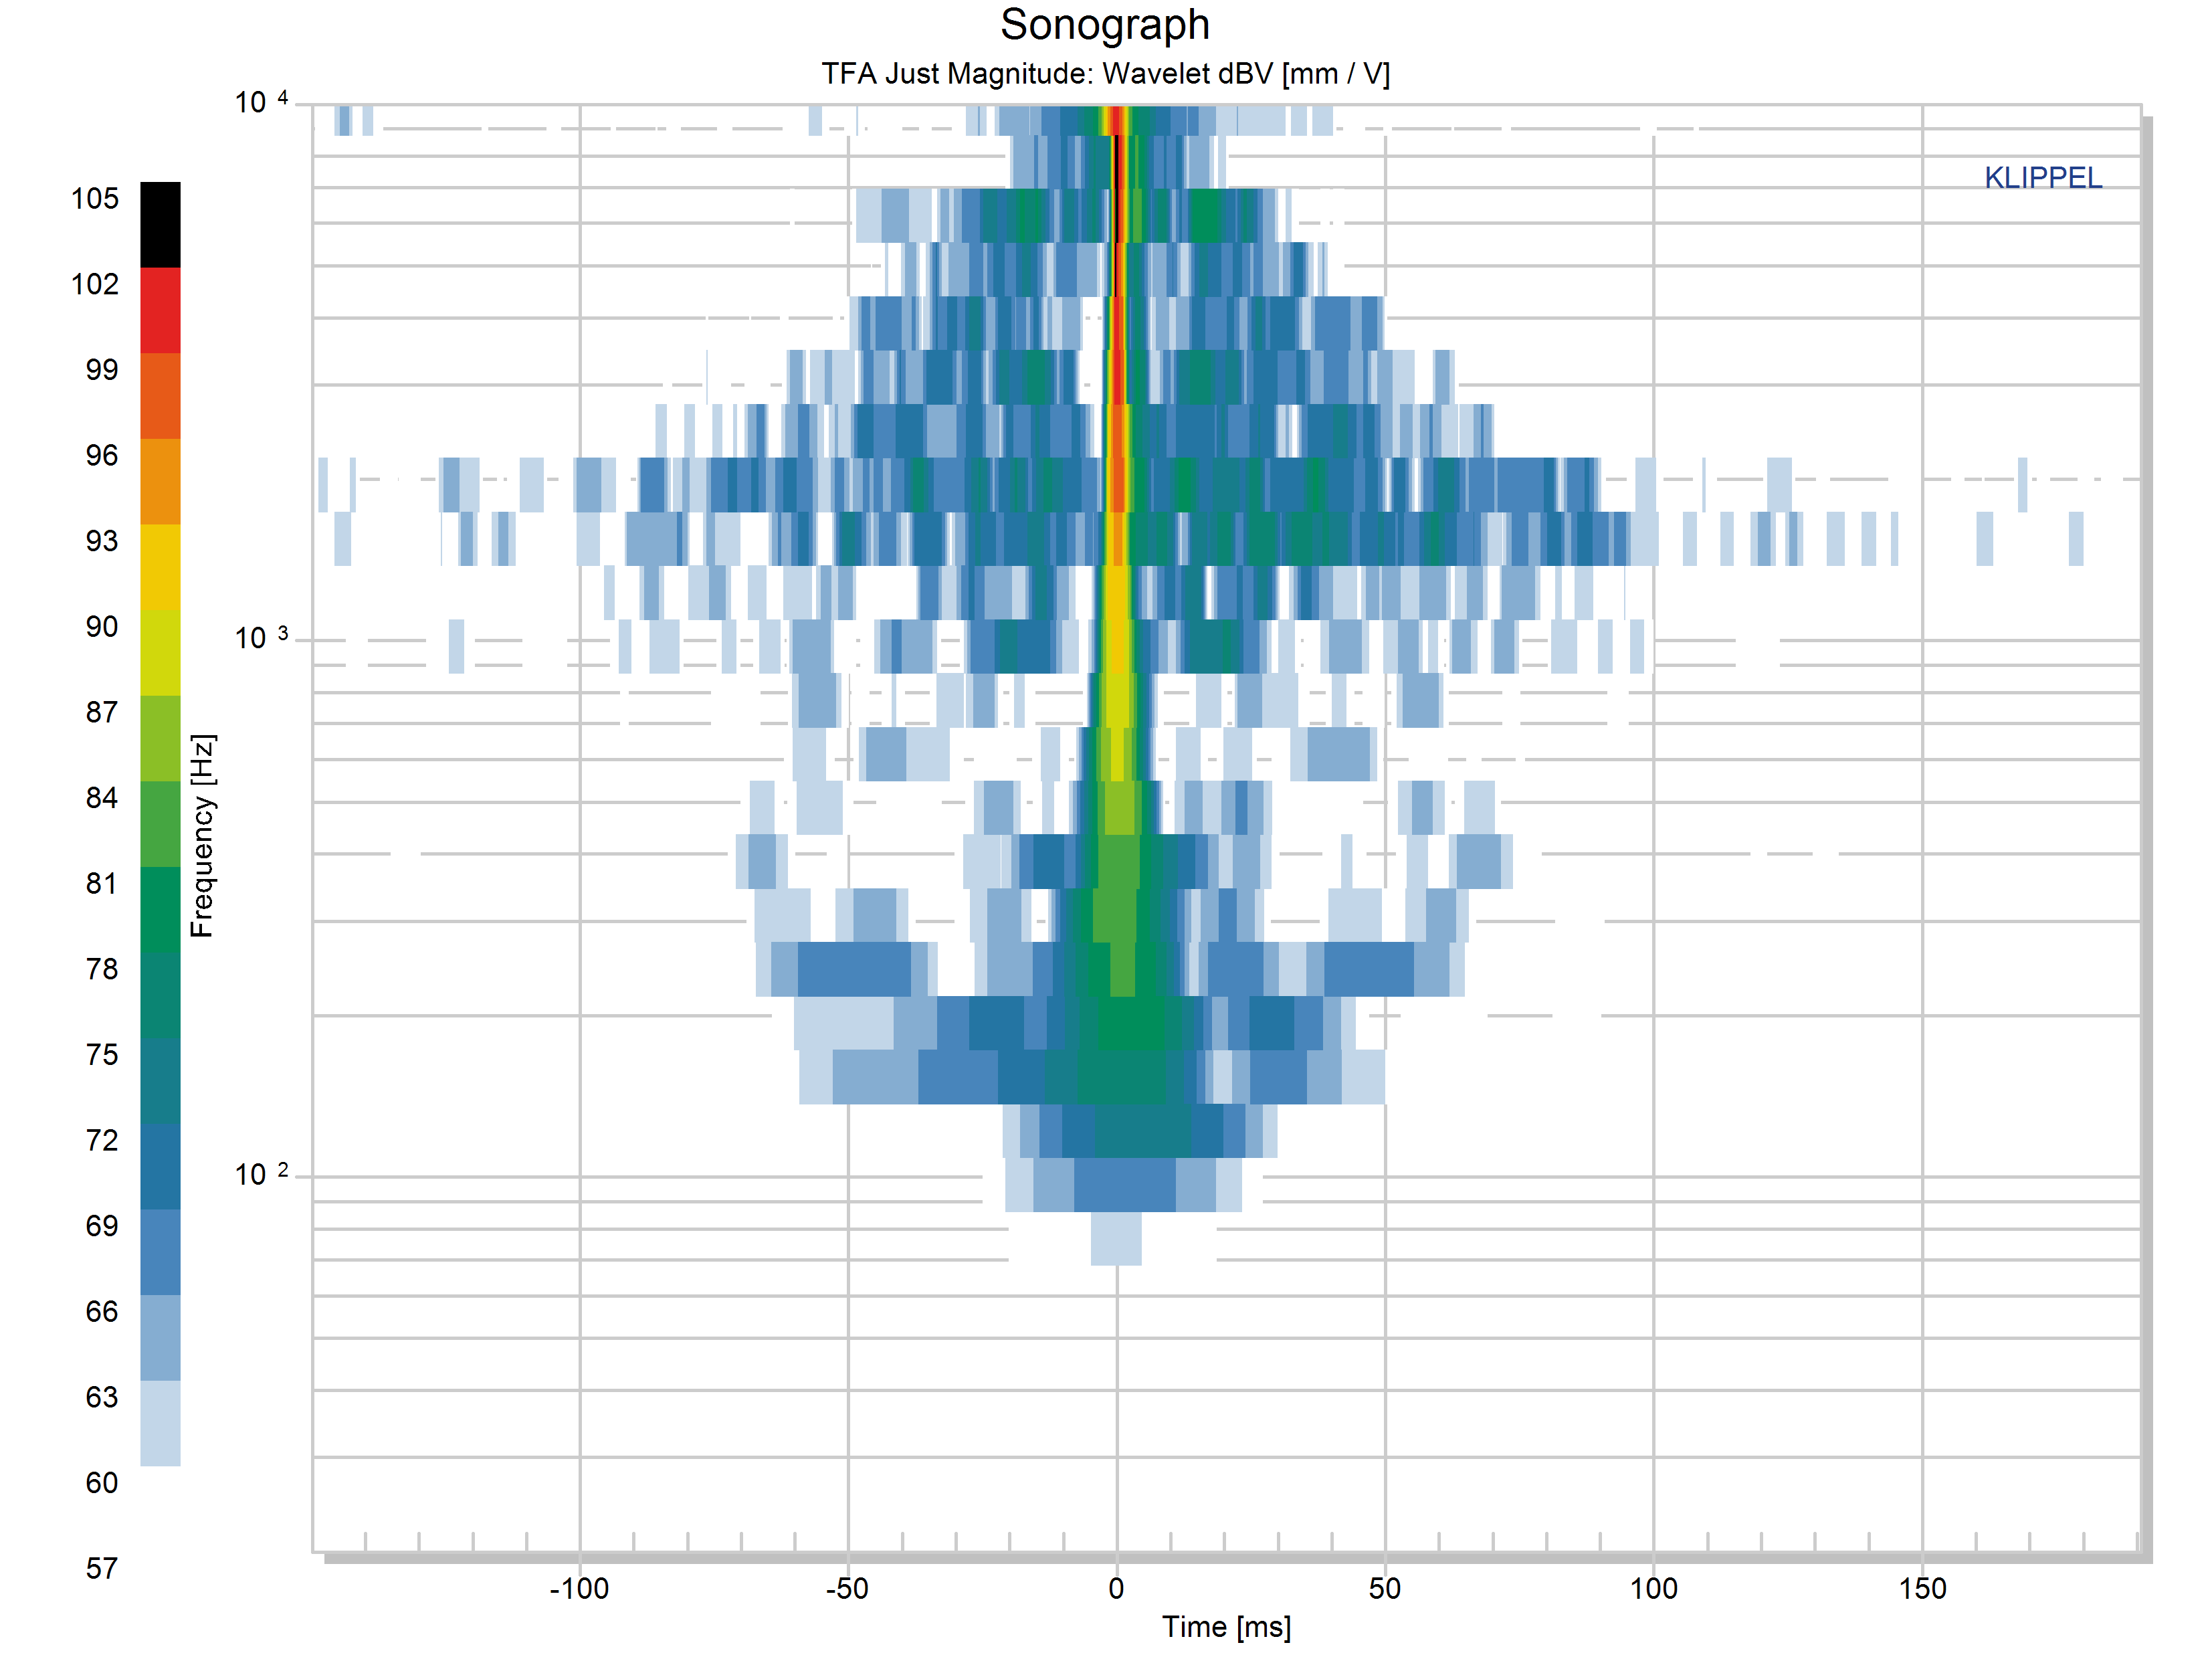
\includegraphics[width=0.95\textwidth]{RoomComp/Sonograph_MagFilt} 
    \captionsetup{hypcap=false} 
	\captionof{figure}{Filter on magnitude} 
	\label{fig:comp_mag}
\end{center}
\end{minipage}
\begin{minipage}{0.33\textwidth}
\begin{center}
	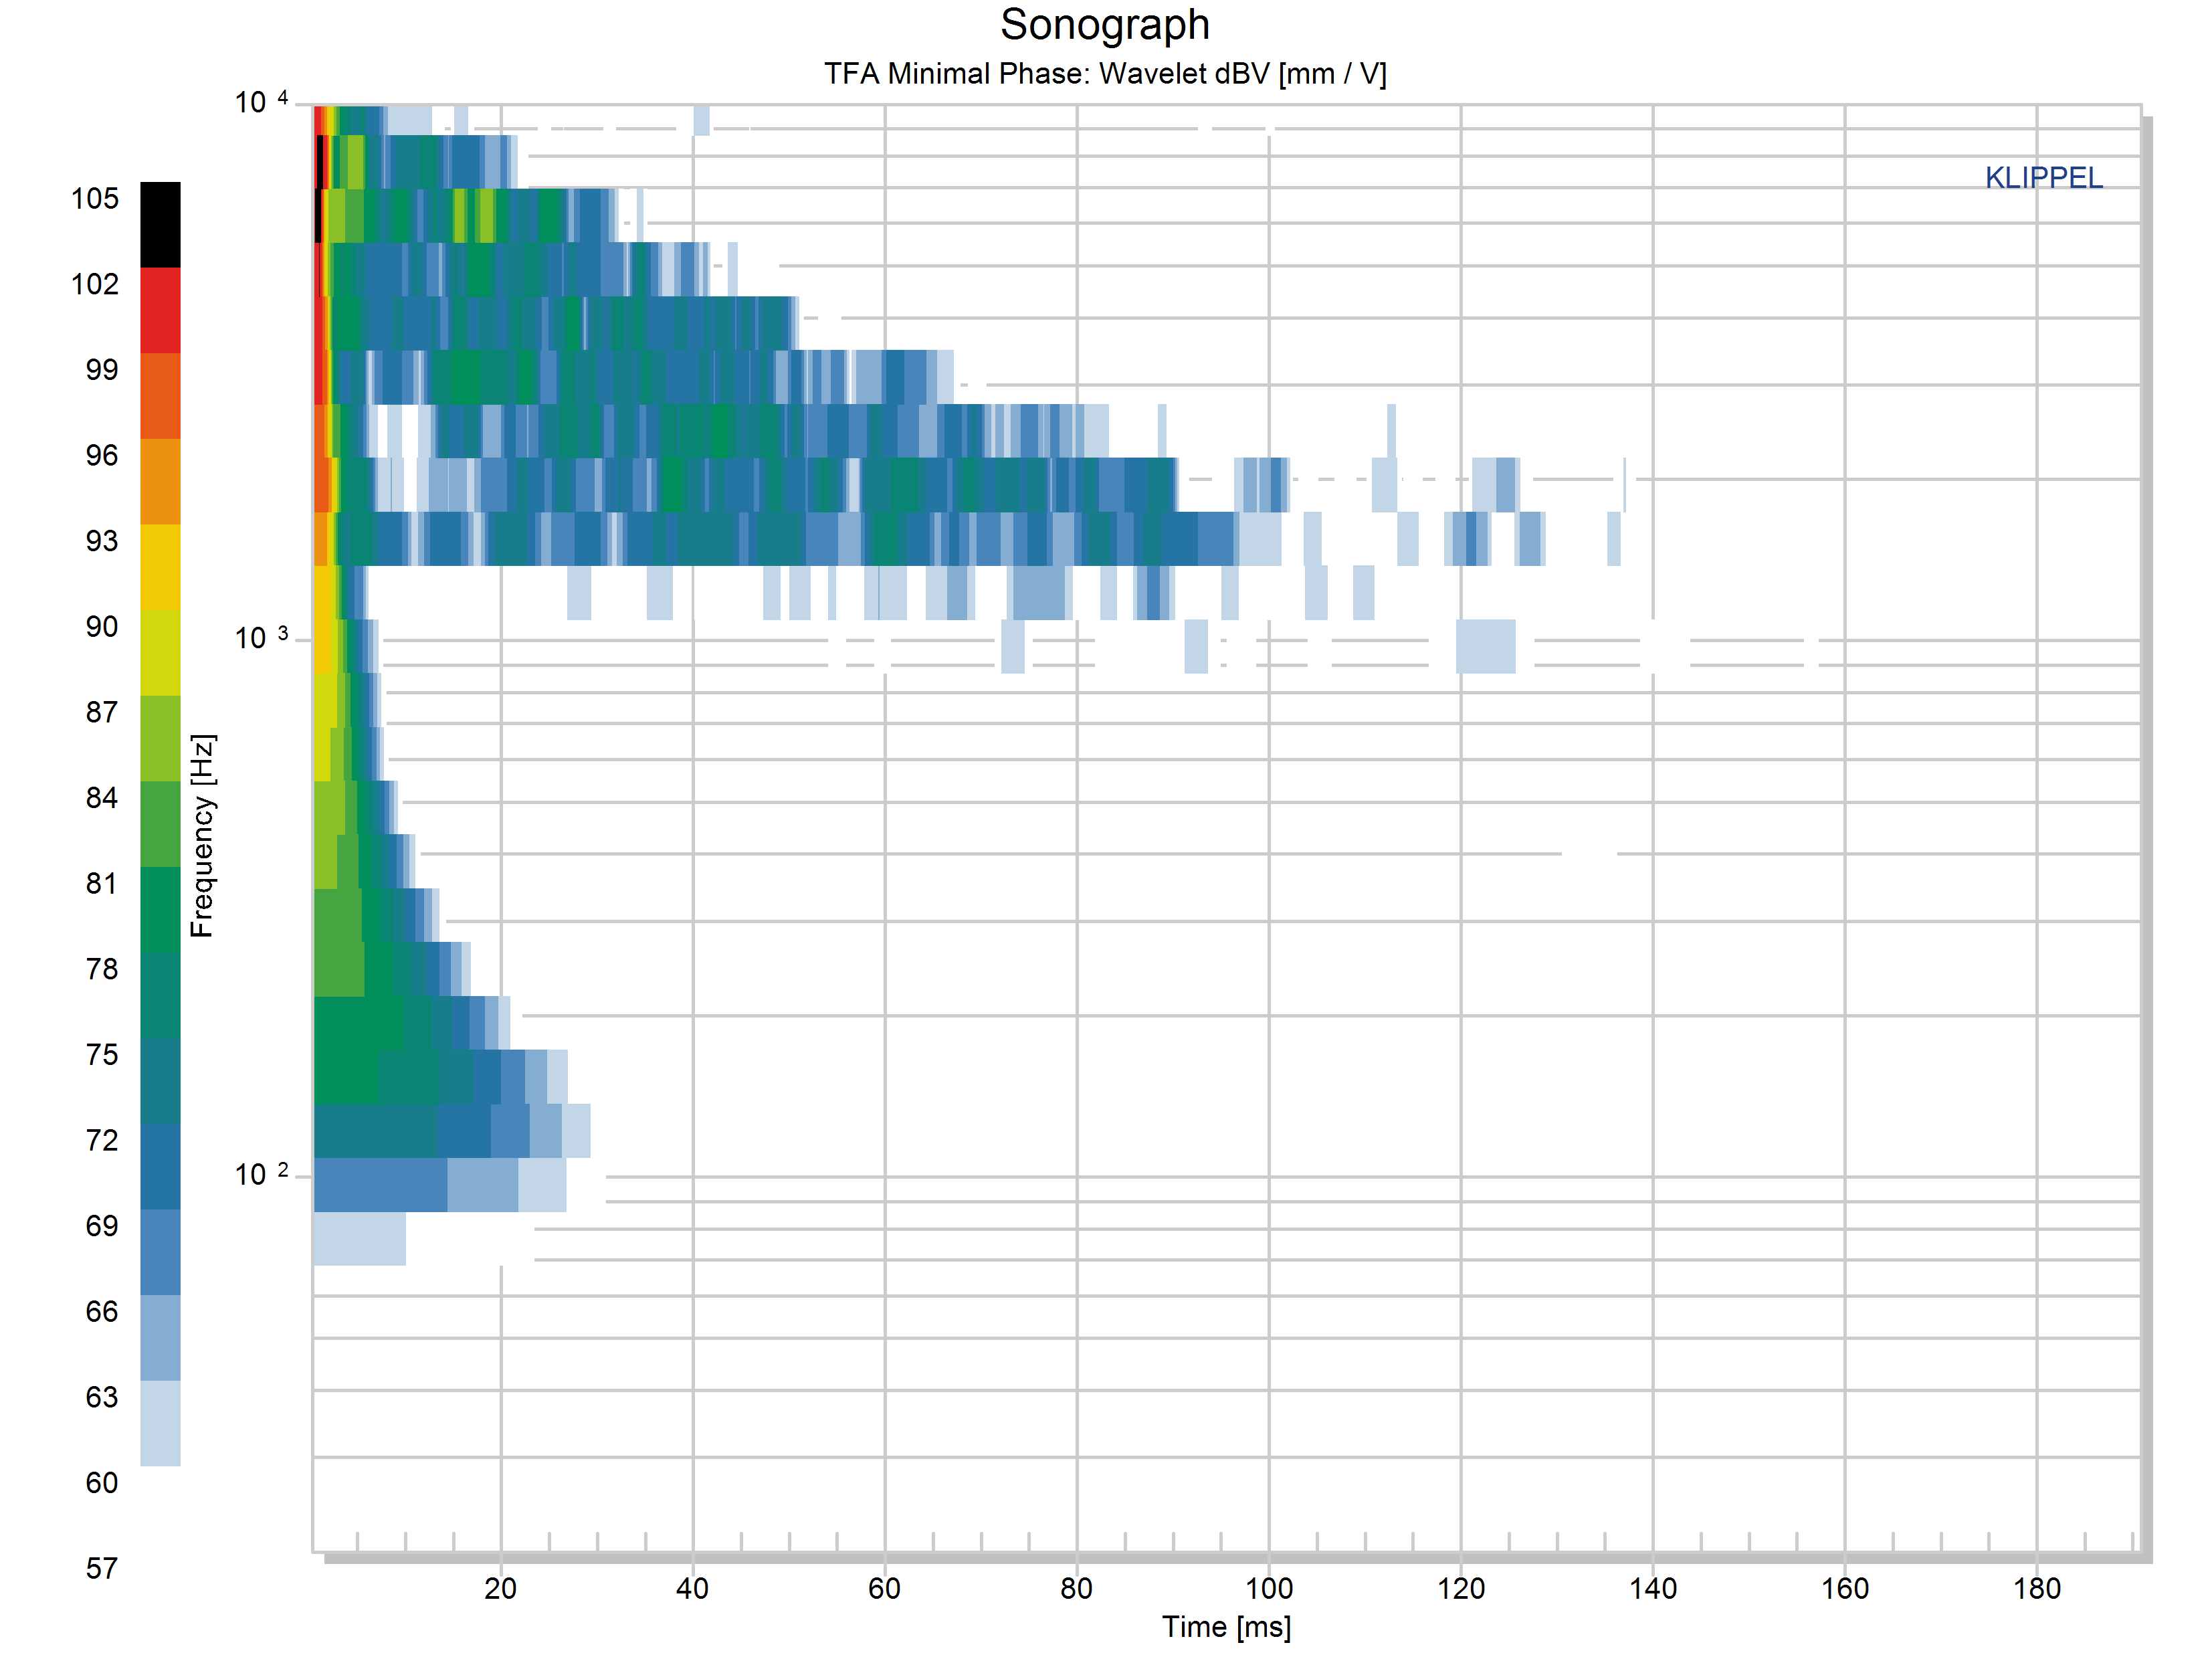
\includegraphics[width=0.95\textwidth]{RoomComp/Sonograph_MinPhase} 
    \captionsetup{hypcap=false} 
	\captionof{figure}{Filter with minimal phase} 
	\label{fig:comp_minphase}
\end{center}
\end{minipage}
\begin{minipage}{0.33\textwidth}
\begin{center}
	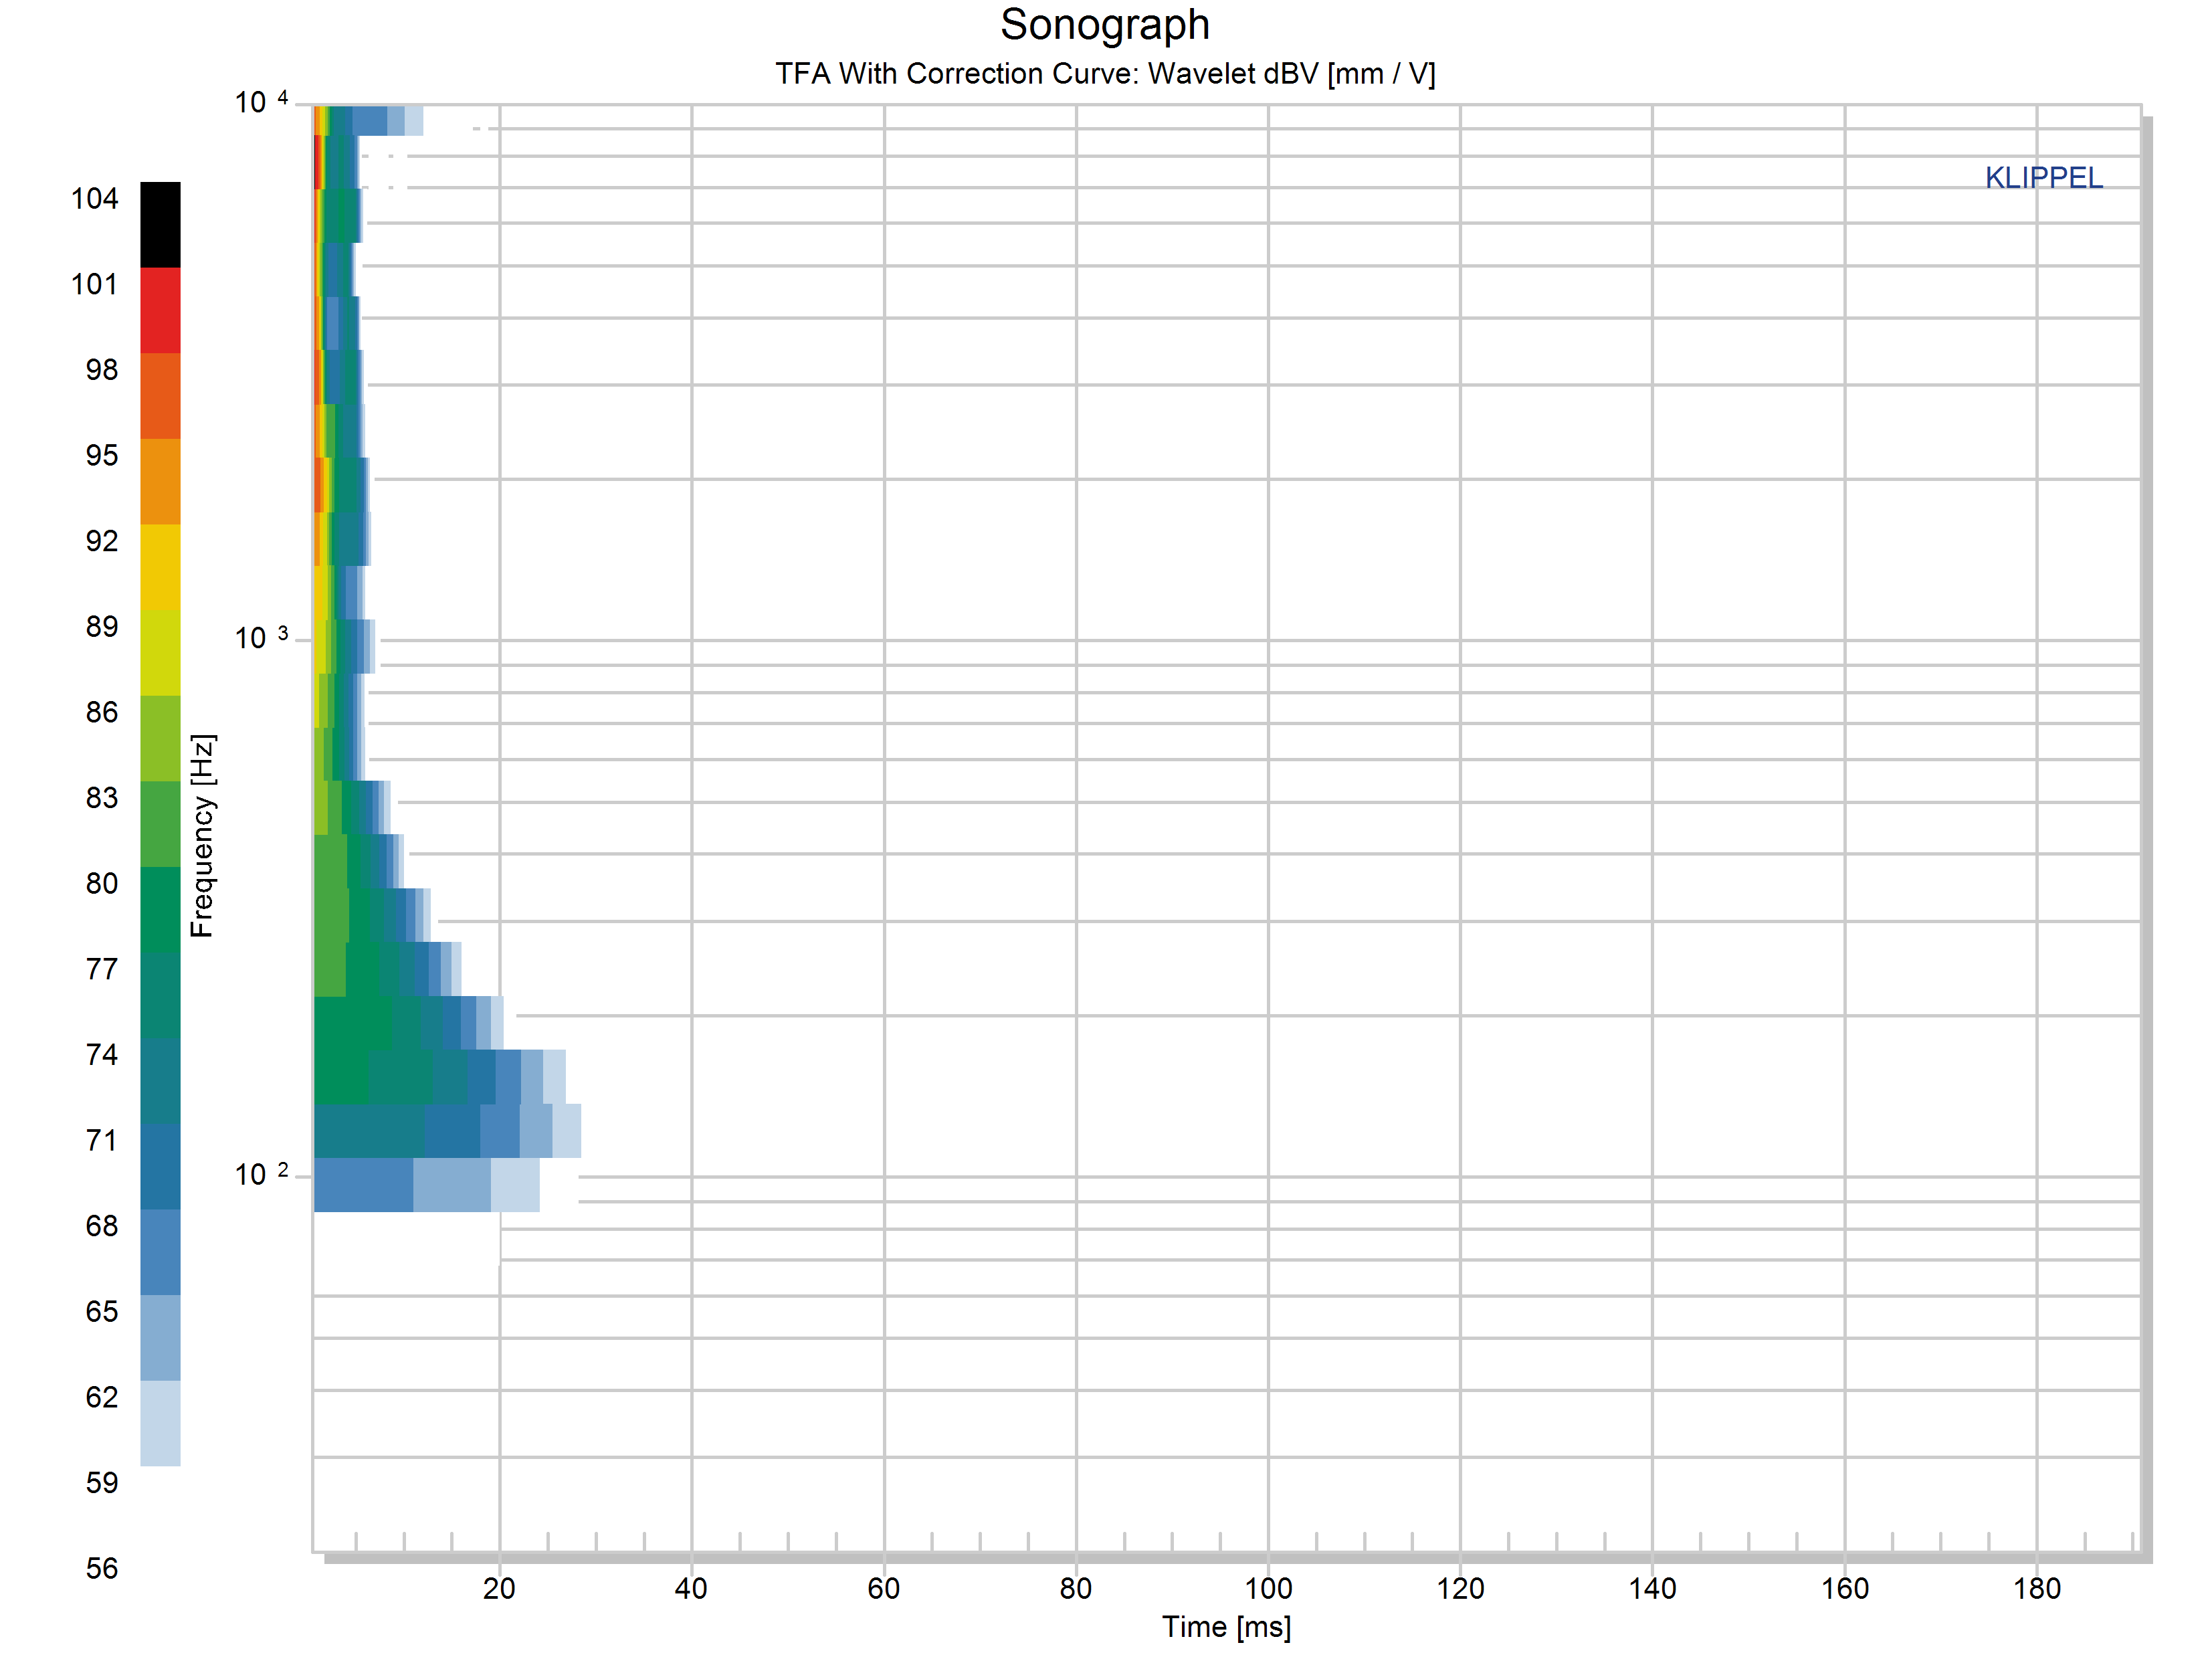
\includegraphics[width=0.95\textwidth]{RoomComp/Sonograph_RoomCor} 
    \captionsetup{hypcap=false} 
	\captionof{figure}{Filter with LFR} 
	\label{fig:comp_RoomCor}
\end{center}
\end{minipage}
\vspace{0.1cm}

Figures \ref{fig:comp_mag}, \ref{fig:comp_minphase} and \ref{fig:comp_RoomCor} presents the Time-Frequency Analysis (TFA) of three different methods to perform a room correction, applied on the measurement of the 10 cm woofer (see \ref{spkrlib:10cm}) Transfer Function (TRF) in free air.
\begin{description}
\item[Figure \ref{fig:comp_mag}] a pre-filter have been applied on the magnitude of the TRF. This method is the most straight-forward but generates ringing artifacts on the TFA: the filter is only applied to the magnitude and does take the phase between the correction curve and the measured curve in consideration. 
\item[Figure \ref{fig:comp_minphase}] the same pre-filter have been applied on the TRF, including the minimal phase that have been reconstructed from the cepstrum of the TRF. Reconstructing the minimal phase enhances the accuracy of the correction in low frequency. However, in high frequencies this method does not dissociate the room from the speaker's contributions, and some ringing can still be observed.
\item[Figure \ref{fig:comp_RoomCor}] the TRF have been post-filtered by a Room Correction curve calculated using the Low-Frequency Reference method described in \citep[][sect.~4]{aeswb}. This method provides the best result: by using a reference curve provided by a measurement of the woofer using the NFS, the phase response of the room can be isolated from the measurement, removing the ringing artifacts visible on the TFA. 
\end{description}


\section{Measurements in the tetrahedral box}

\subsection{Influence of the load}

The tetrahedral test box being a closed box system, it will have an impact on the speaker's behavior. Closed box can be approximated as an additional  stiffness on the speaker's equivalent network, due to the springiness of the air volume trapped in the box. This effect is mostly present in low frequency, as shown in figure \ref{fig:Load_Compa}: the blue curve is the measure in the box and the orange curve the result of the NFS of the 10 cm woofer (see appendix \ref{spkrlib:10cm}). In the 20 Hz - 150 Hz range the box creates a "bass boost" effect. \\

Assuming that the driver is in the linear range, the displacement transfer function of a driver in free air is given by equation \ref{eq:TRF_disp}, where $ e_{g}$ is the input voltage, $C_{ms}$ the compliance, $Bl$ the force factor, $\omega_{s}$ the resonance frequency of the system, and $Q_{ts}$ the total quality factor of the system.

\begin{equation}
x(\omega ) = e_{g}\cdot \frac{C_{ms}Bl}{R_{e}}\cdot \frac{1}{(j\omega /\omega _{s})^{2}+(1/Q_{ts})(j\omega /\omega _{s})+1}
\label{eq:TRF_disp}
\end{equation}
\myequations{Displacement transfer function in free air}

Figure \ref{fig:eq_circ} represents the simplified equivalent circuit of the driver in the box. The effect of the box is represented by the compliance $C_{box}$. $e_{g}$ represents the input voltage, $R_{e}$ the electrical resistance; $R_{ms}$, $C_{ms}$ and $M_{ms}$ the mechanical parameters of the driver and $Bl$ the force factor.

\begin{figure}[ht]
	\begin{center}
	\begin{circuitikz}
		\draw
  	 	 (2,2) node[gyrator] (T) {}
    (T.A2)  -- + (-2,0) coordinate (aux1)
            to[V^=$e_{g}$]    (aux1  |- T.A1) 
            to[generic,l=$R_{e}$] (T.A1)           
    (T.B1)  to[R=$R_{ms}$] + (2,0)
            to[C=$C_{ms}$] + (2,0)
            to[L=$M_{ms}$] + (2,0)
            to[C=$C_{box}$] + (0,-2) |- (T.B2)
    (T.base) node{Bl:1};
	\end{circuitikz}
	\caption{Equivalent circuit of a driver in the box}
	\label{fig:eq_circ}
	\end{center}
\end{figure}

From equation \ref{eq:TRF_disp} and the equivalent circuit presented by figure \ref{fig:eq_circ} the displacement transfer function of the system in the box can be expressed by equation \ref{eq:TRF_dispbox}. $C_{msb}$ is the equivalent compliance of the system in the box such as $C_{msb} = C_{ms} + C_{box}$ and $e_{gb}$ the input voltage.

\begin{equation}
x_{b}(\omega ) = e_{gb}\cdot \frac{C_{msb}Bl}{R_{e}}\cdot \frac{1}{(j\omega /\omega _{s})^{2}+(1/Q_{ts})(j\omega /\omega _{s})+1}
\label{eq:TRF_dispbox}
\end{equation}
\myequations{Displacement transfer function in the box}

To correct the effect of the box, an input voltage for which $x(\omega )$ = $x_{b}(\omega ) $ can be calculated as given in equation \ref{eq:V_corr} where $K_{ms}$ and $K_{msb}$ are the stiffness in free air and in the box respectively, such as $K_{ms}$ = $\frac{1}{C_{ms}}$.

\begin{equation}
e_{gb} = e_{g}\cdot \frac{C_{ms}}{C_{msb}} = e_{g}\cdot \frac{K_{msb}}{K_{ms}}
\label{eq:V_corr}
\end{equation}
\myequations{Voltage correction for the box}

This voltage can be expressed as a function of the resonance frequency given by equation \ref{eq:fs}, where $M_{ms}$ is the moving mass of the driver. 

\begin{equation}
f_{s} = \frac{1}{2 \pi \sqrt{\frac{M_{ms}}{K_{ms}}}}
\label{eq:fs}
\end{equation}
\myequations{Resonance frequency of a speaker}

Expressing the voltage as a function of the resonance frequency makes the compensation easier to estimate, as the calculation of the Thiele \& Small parameters is no longer required. From a simple electrical measurement of the impedance, which is the ratio of the output voltage by the output current $Z = U_{s}/I_{s}$, the resonance frequency can be found at the maximum of the impedance. 

\begin{equation}
e_{gb} = e_{g}\cdot \frac{(2 \pi f_{s})^{2}}{(2 \pi f_{b})^{2}}
\label{eq:V_corr_fs}
\end{equation}
\myequations{Voltage correction for the box as a function of resonance frequency}

Equation \ref{eq:V_corr_fs} gives the compensated voltage for the box, where $ f_{s}$ is the resonance frequency of the driver in free air and $ f_{b}$ the resonance frequency of the driver in the box. This implies that 2 measurements are required: one of the driver in free air, and one of the driver in the box. \\
Now that the theory is expressed, this assumptions needs to be verified. To do so, the impedance of the driver and the displacement transfer function of the driver's membrane have been measured on the 10 cm woofer by using the Klippel system, and with a laser pointing on the driver's membrane estimates the displacement. \\

\begin{minipage}{0.5\textwidth}
\begin{center}
	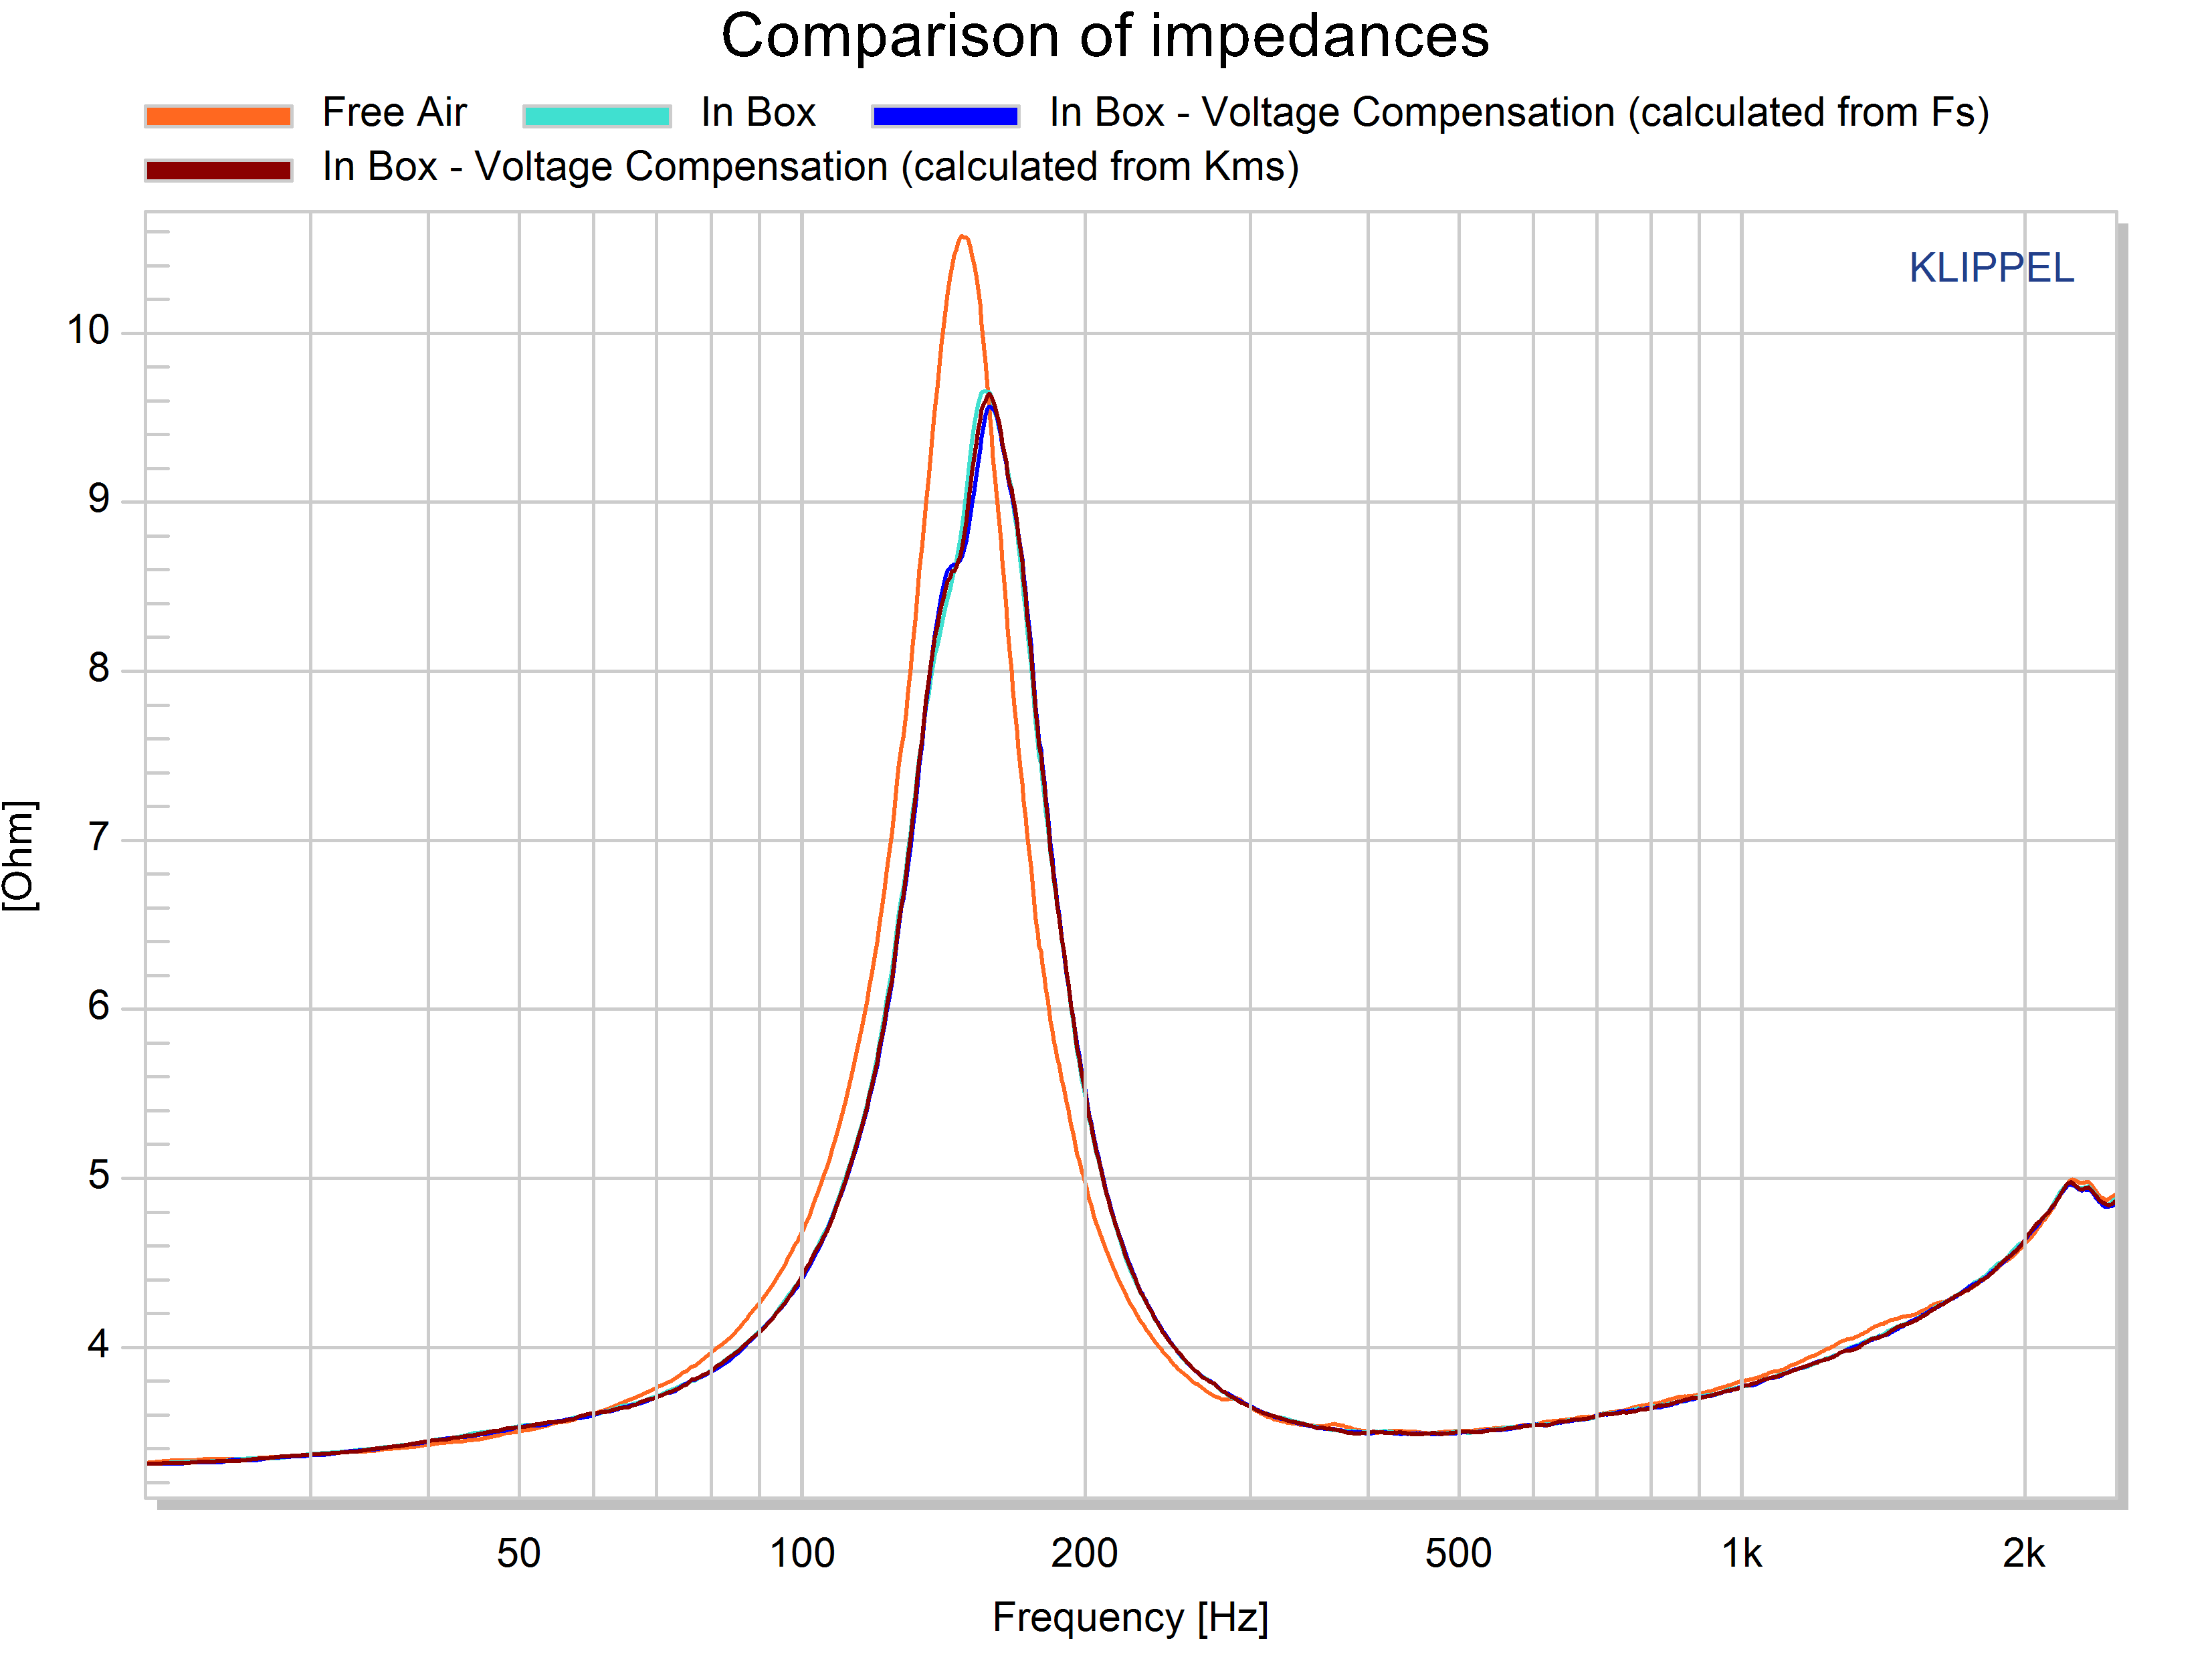
\includegraphics[width=0.9\textwidth]{RoomComp/Imp_Comps} 
    \captionsetup{hypcap=false} 
	\captionof{figure}{Comparison of measured impedance} 
	\label{fig:imp_comp}
\end{center}
\end{minipage}
\begin{minipage}{0.5\textwidth}
\begin{center}
	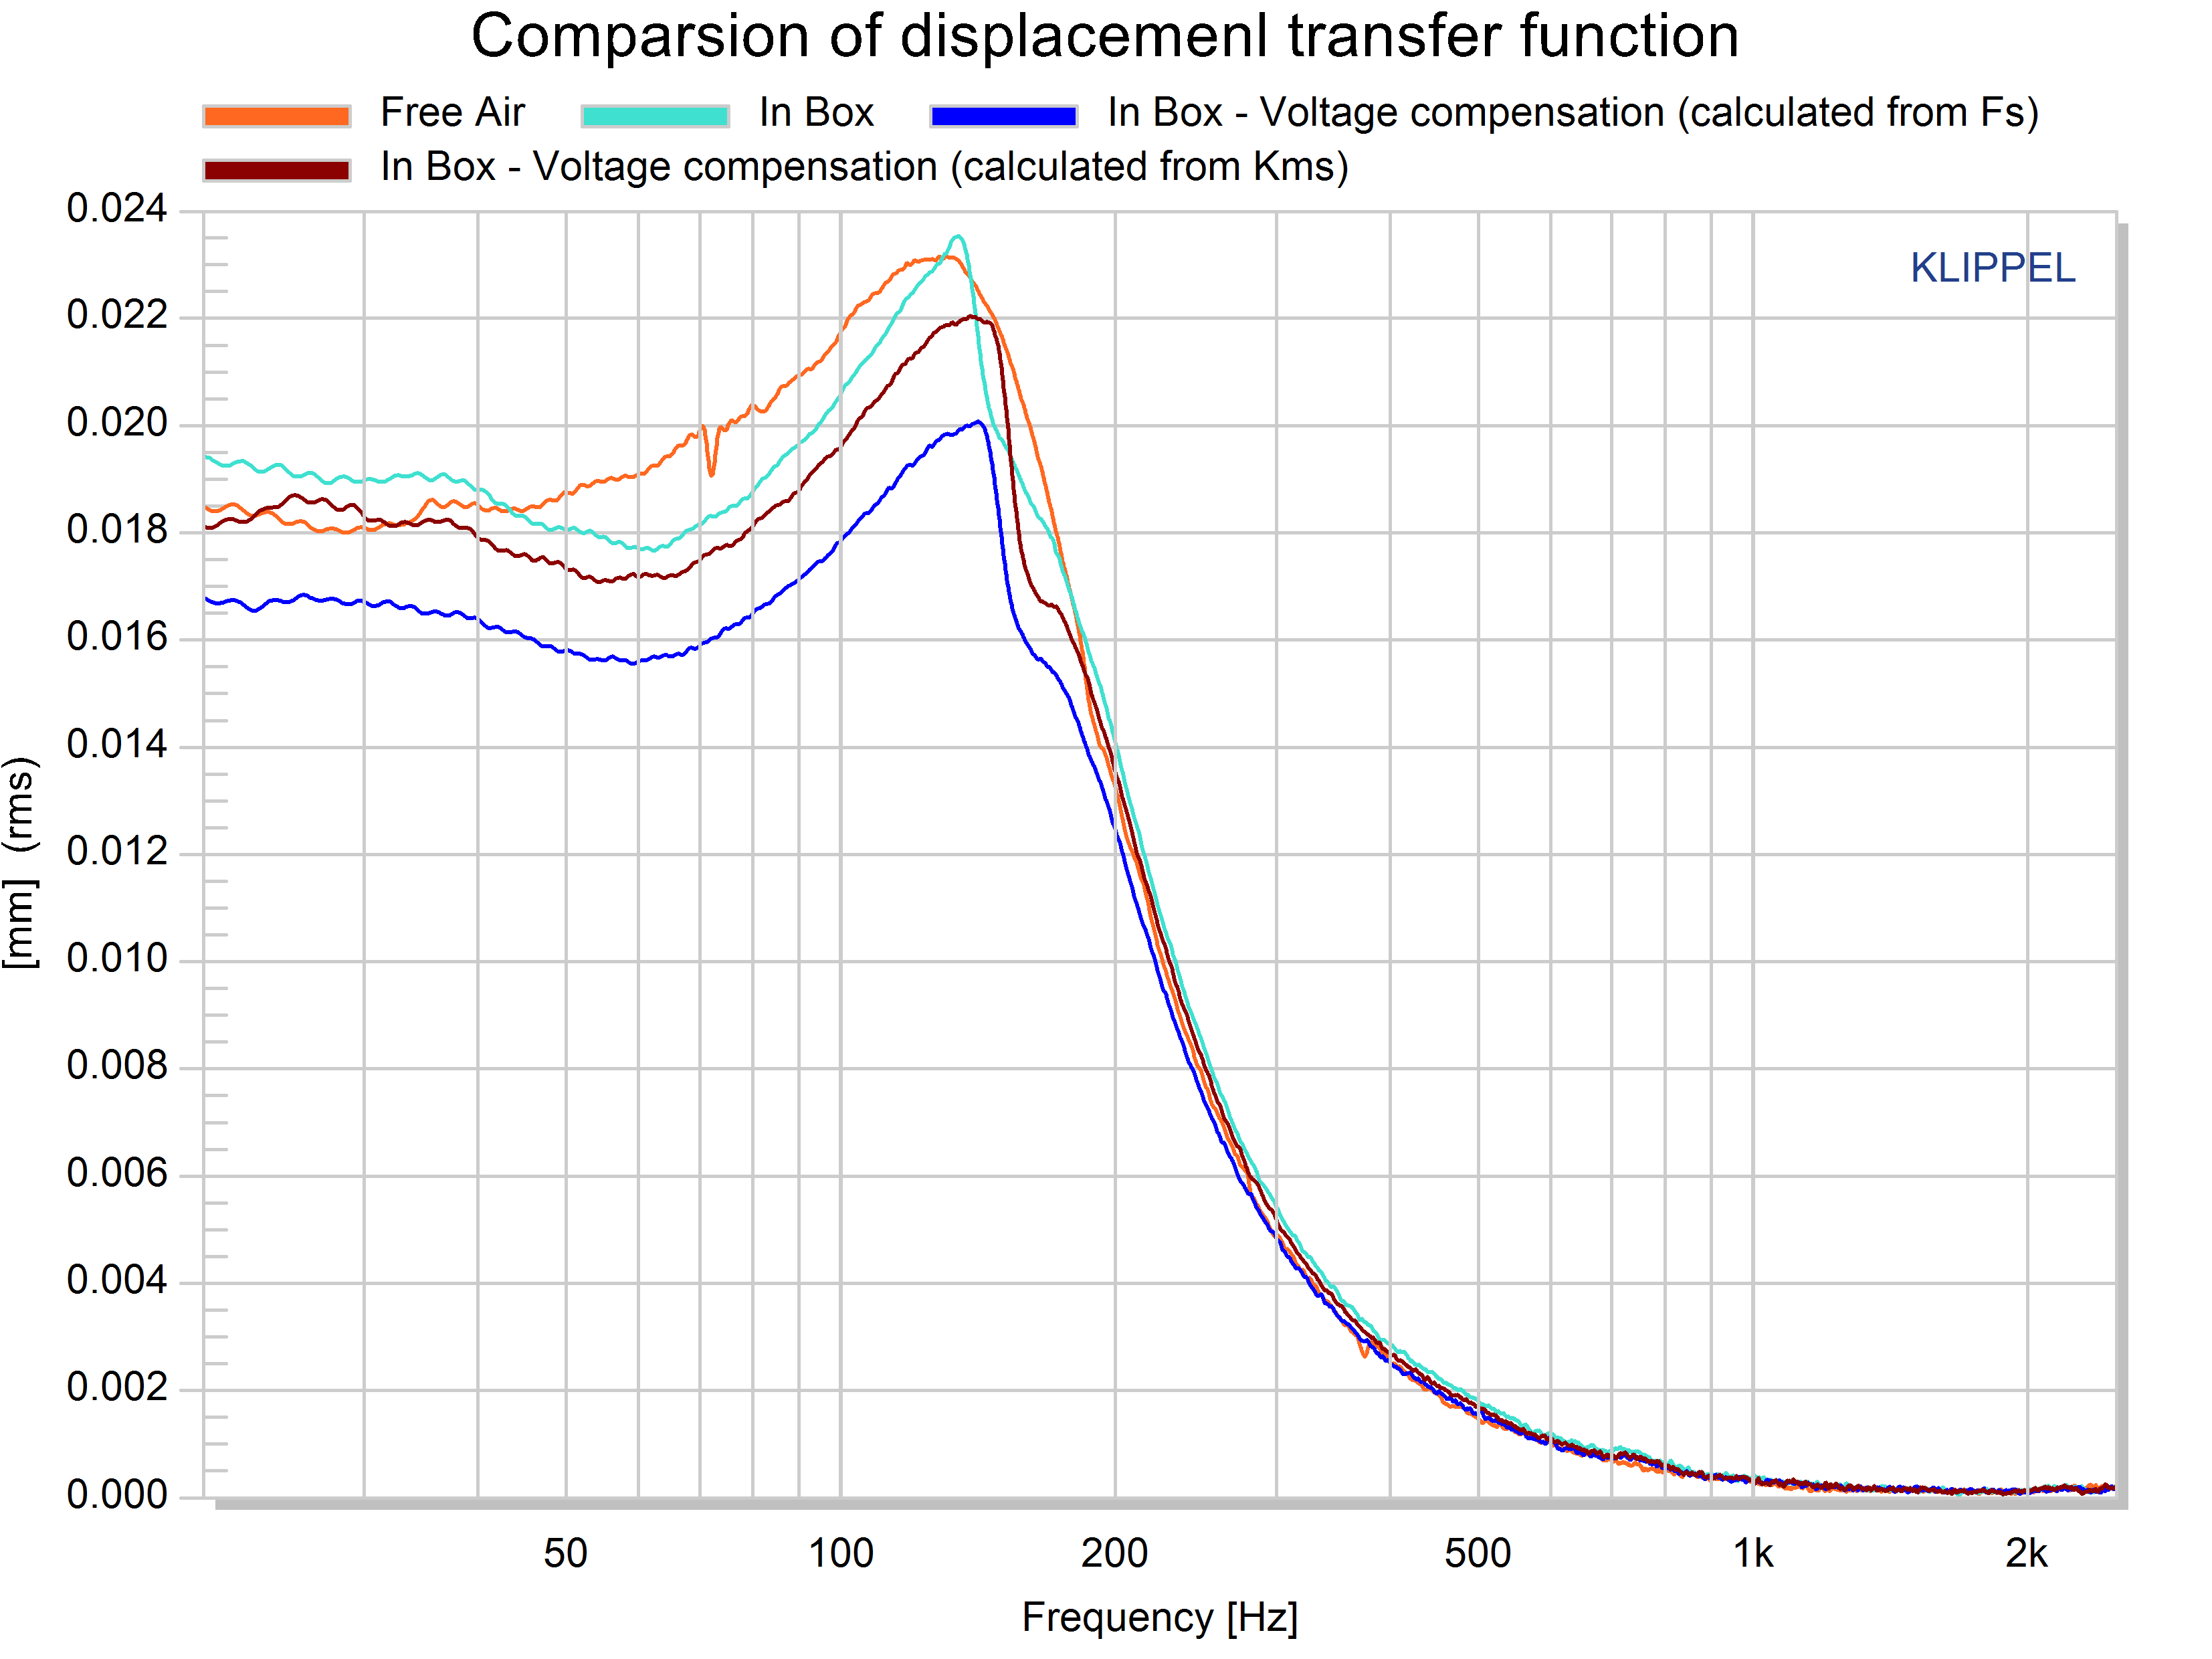
\includegraphics[width=0.9\textwidth]{RoomComp/Disp_Comps} 
    \captionsetup{hypcap=false} 
	\captionof{figure}{Comparison of measured displacement TRF} 
	\label{fig:disp_comp}
\end{center}
\end{minipage}
\vspace{0.1cm}

Figure \ref{fig:imp_comp} presents the comparison of the measured impedances for different conditions: the initial measures in free air and in the box to estimate the voltage compensation to apply, and the results of the new measurements when the voltage compensations is calculated from the $K_{ms}$ (measured using Klippel's laser method for Thiele \& Small parameters estimation) and the $f_{s}$ (measured at the maximum of the impedance curves) have been applied. \\
When looking at this results, few differences between the impedance in the box and the corrected curves can be found. However, when looking at the displacement transfer functions presented in figure \ref{fig:disp_comp}, interesting results are found. \\

Comparing the free air and in box measurement shows that up to 50 Hz the membrane's displacement is greater in the box, generating the "bass boost" effect observed before (figure \ref{Curves:InfluLoad}). The displacement is then larger in free air than in the box, expect at the driver's resonance.\\
Using the voltage correction calculated either by the ratio of resonance frequencies $f_{s}$ and $f_{b}$ or the ratio of stiffness $K_{ms}$ lowers the membrane's displacement in the box, although the attenuation provided by the ratio of resonance frequencies is overestimated: the membrane's displacement is too attenuated in the 20 - 500 Hz frequency band. The attenuation provided by the ratio of stiffness gives promising results, particularly in the "bass boost" frequency band (20 - 50 Hz) and around the resonance, where the displacement transfer function in the box gets close to the one measured in free air. \\

The mismatches between the free air and voltage compensated curves are most likely due to the approximations made on the box's behavior. The effect of the box of the driver is much more complicated than a change on the mechanical compliance, especially since leakage isn't taken in account.  

\todo[inline, color=red!40]{Expliquer que les différences sont dues à l'approximation trop simpliste sur le modèle de la boite, mais bien formulé. Ajouter les schémas équivalents + citer J. Panzer (cours transducer basics / Acoustics / LEM Sealed Box)}

\subsection{Influence of microphone position}

Investigating the influence of the microphone position allows to deduce how critical this parameter is, and how to ensure a correct microphone positioning. Several measurements of the 10 cm woofer (see appendix \ref{spkrlib:10cm}) have been performed for different microphone - speaker distances $D_{ms}$. A schematic of the measurement is given in figure \ref{fig:micpos_schema}.  \\

Figure \ref{fig:MicPosTRF} shows the transfer functions obtained for different distances $D_{ms}$ (see figure \ref{fig:micpos_TRF_big} for a bigger version). In low frequencies up to 150 Hz, the transfer functions are similar. After 150 Hz strong differences appear between the transfer functions. The larger the distance $D_{ms}$ is and the bigger the box influences the measurement, generating a dip on the response at around 1 kHz. This phenomenon is believed to be the first box mode and is observed when measuring different speakers. \\
\todo[inline, color=red!40]{mieux formuler + tirer des conclusions etfaire le lien avec les autres figures}
\begin{minipage}{0.35\textwidth}
\begin{center}
	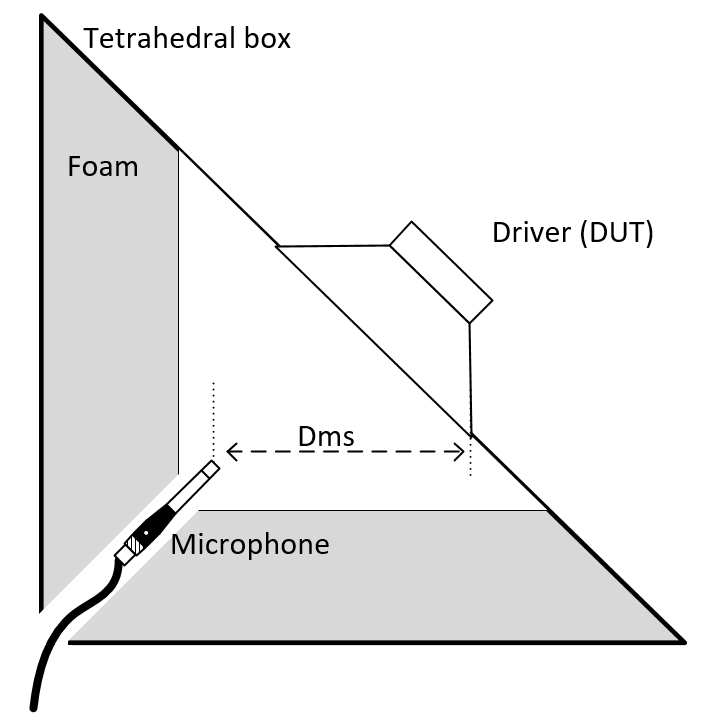
\includegraphics[width=0.9\textwidth]{RoomComp/Mic_Pos_Schm} 
    \captionsetup{hypcap=false} 
	\captionof{figure}{Microphone position} 
	\label{fig:micpos_schema}
\end{center}
\end{minipage}
\begin{minipage}{0.6\textwidth}
\begin{center}
	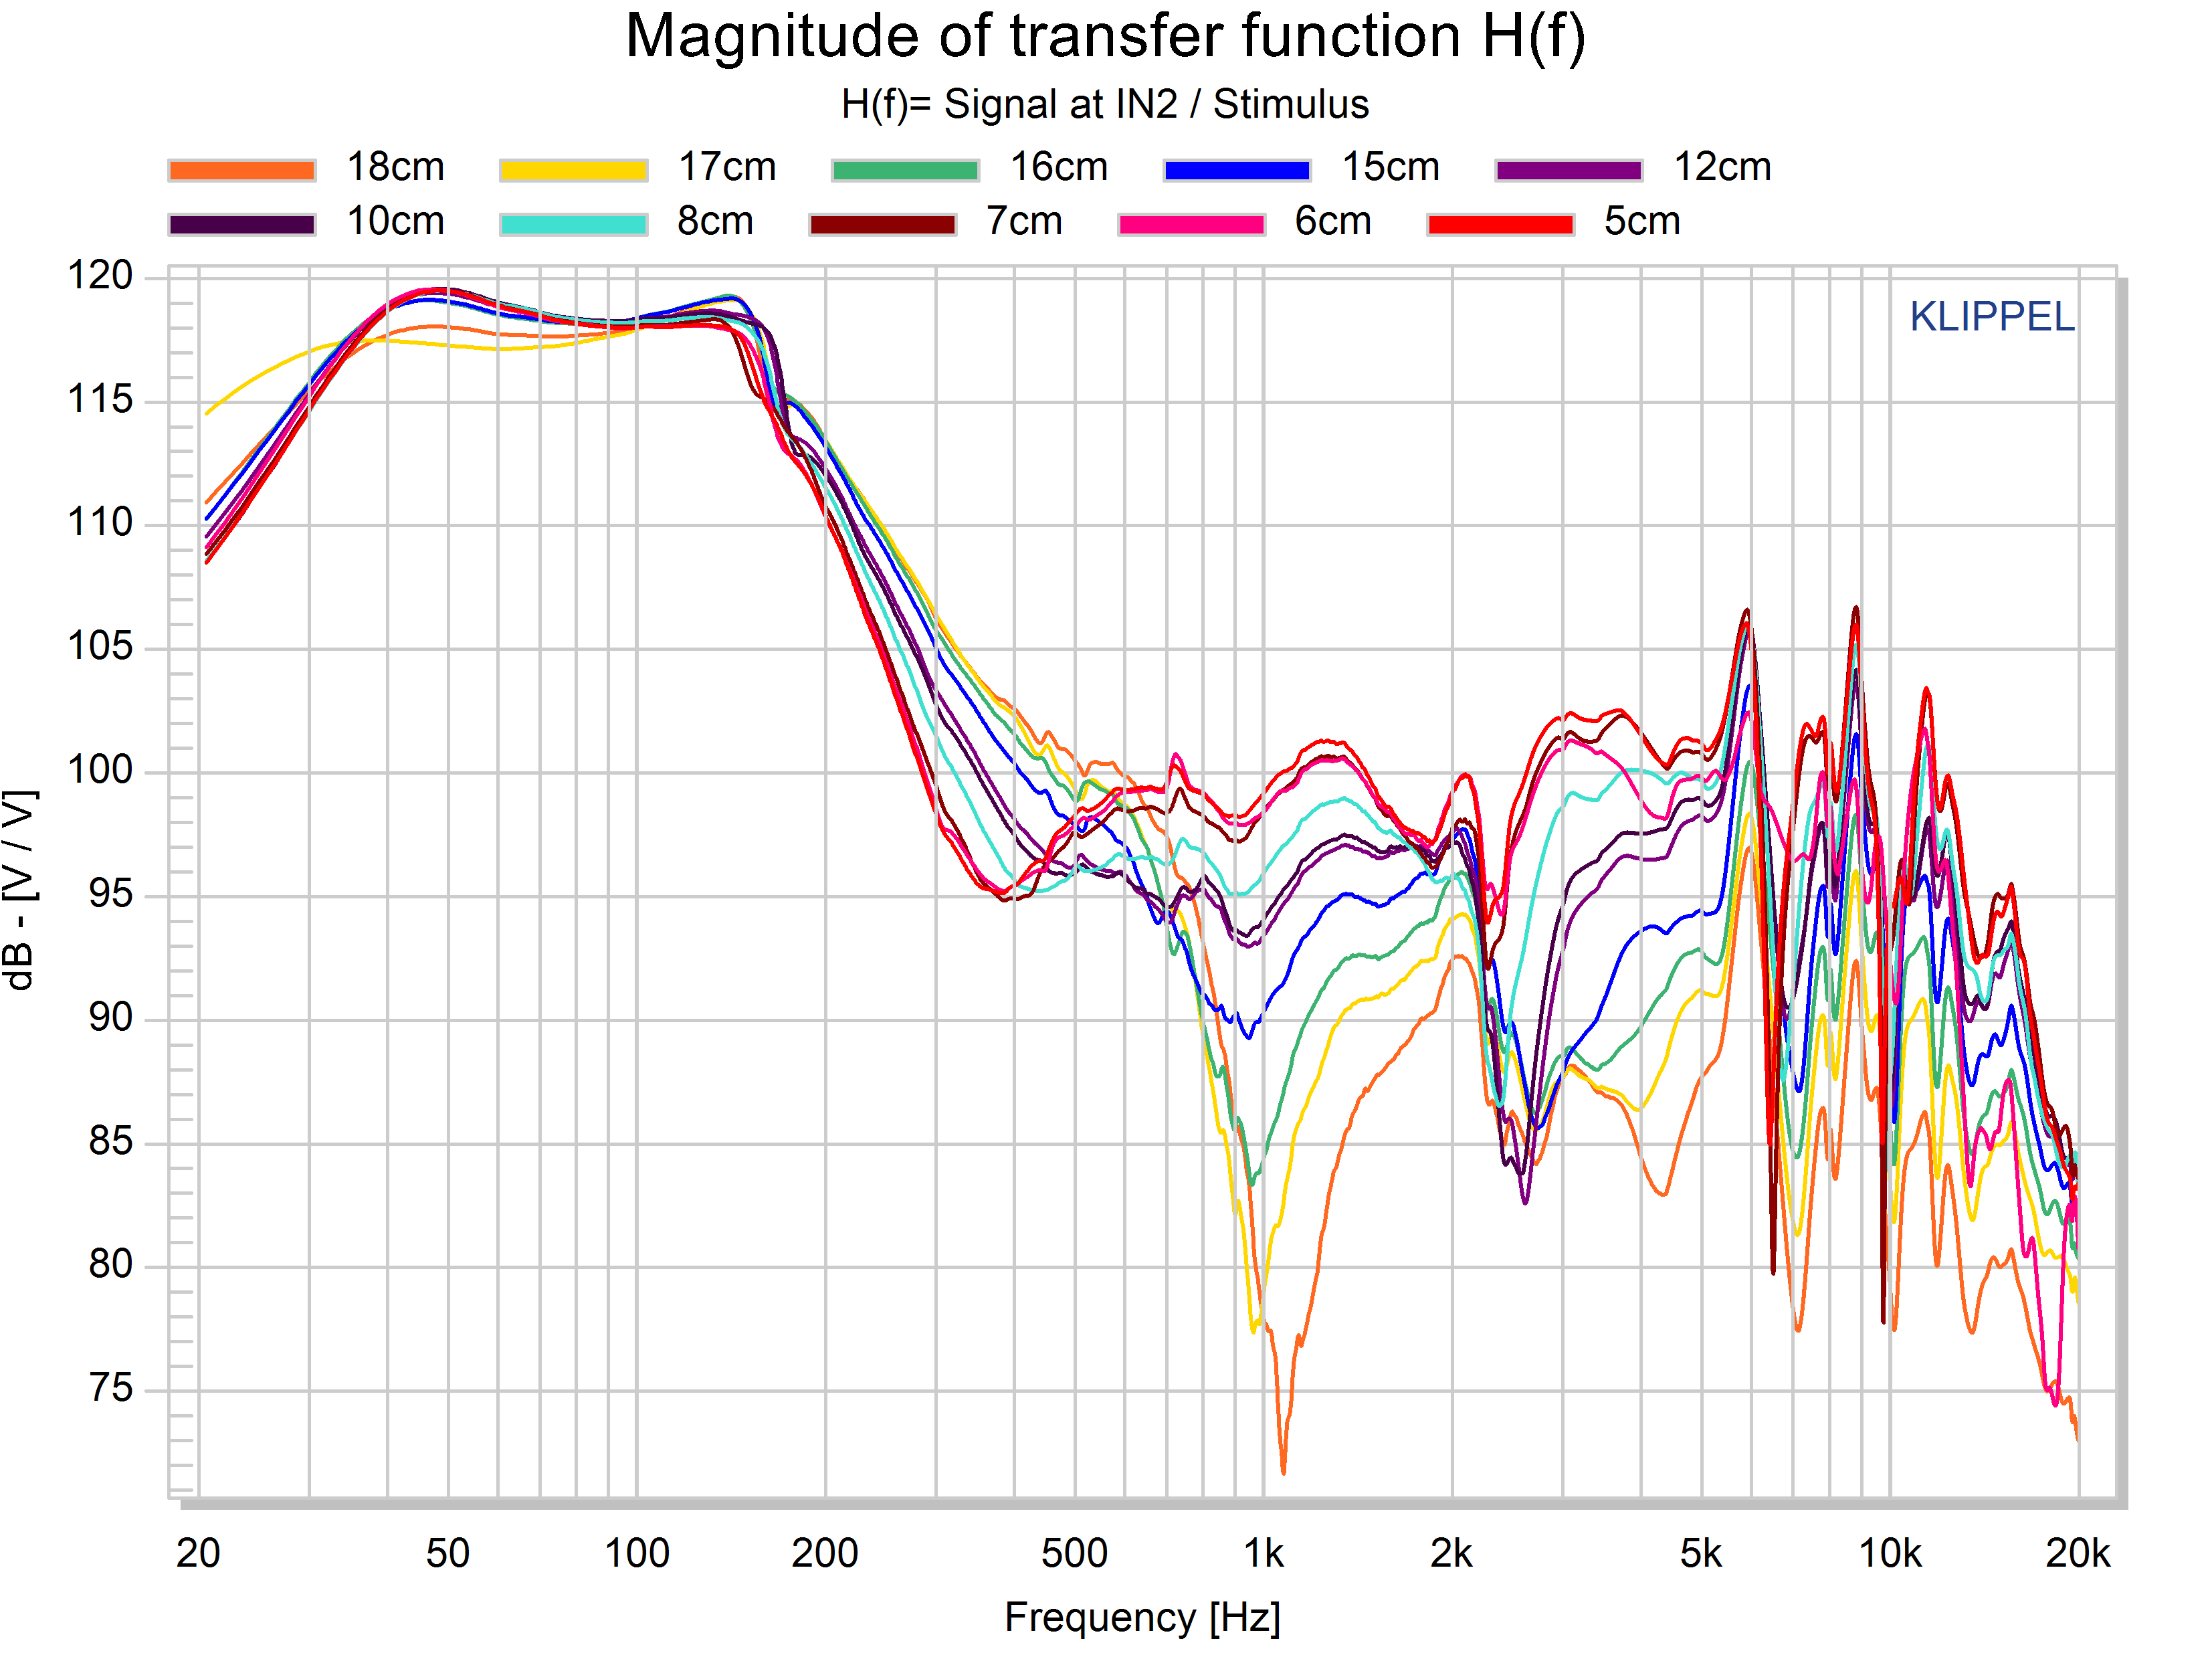
\includegraphics[width=1\textwidth]{RoomComp/MicPos_TRF} 
    \captionsetup{hypcap=false} 
	\captionof{figure}{Transfer Functions for different positions} 
	\label{fig:MicPosTRF}
\end{center}
\end{minipage}
\vspace{0.1cm} 


From this result it can be deduced that there is a critical range for the microphone positioning. Figure \ref{fig:MicPosDiffNFS} shows the differences between the results from the NFS, extrapolated at their respective distances; and the measured transfer functions. This set of curves is the Room Compensation functions, or references. In the 20 Hz - 150 Hz frequency range a "bass boost" is observed, created by the box's air load. This boost can be easily eased off by applying the LFR room compensation method.\\
\todo[inline, color=red!40]{Tu ne parle pas de la bonne figure pour apprécier les différences. La différence entre les RCs est + pertinente car elle devrais être de 0 dB si le mic n'avais pas d'influence}
A zoom on the 150 Hz - 20 kHz is provided in figure \ref{fig:MicPos_Diff_NFS_Zoom}. In this frequency range, the accepted level of differences is $\pm$ 5 dB. The distances $D_{ms}$ satisfying that range are 5 cm, 6 cm and 7 cm. When the microphone is 8 cm away from the speaker the differences are already too critical to ensure an accurate measurement. \\

\begin{minipage}{0.5\textwidth}
\begin{center}
	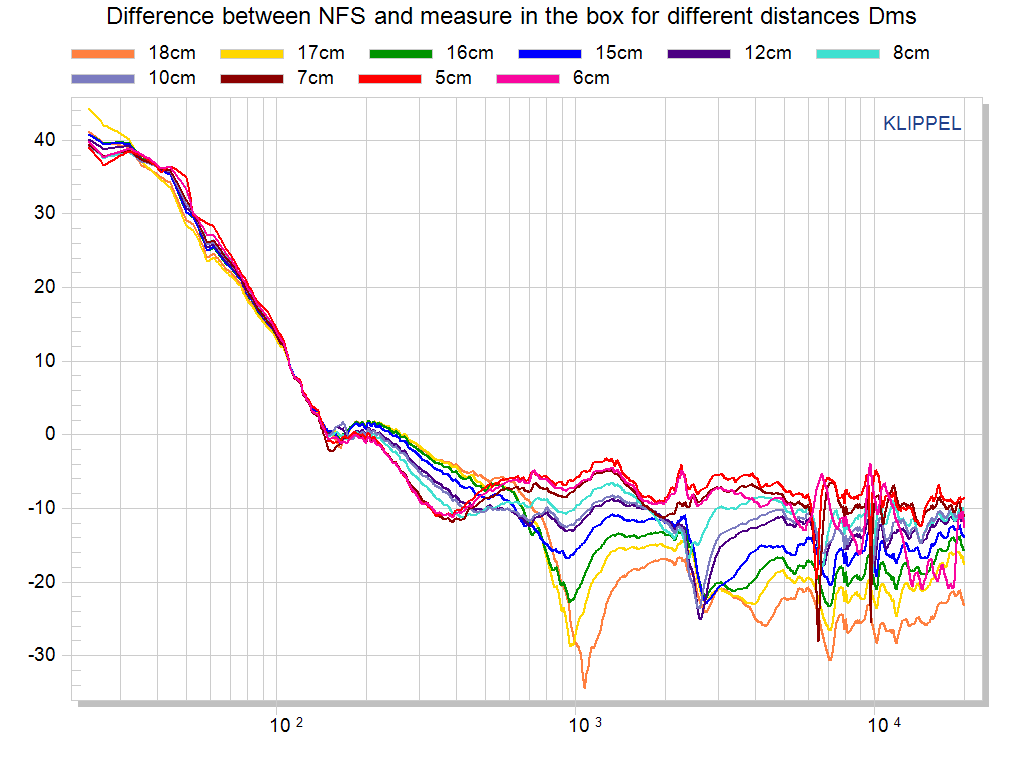
\includegraphics[width=0.9\textwidth]{RoomComp/MicPos_Diff_NFS_TRF} 
    \captionsetup{hypcap=false} 
	\captionof{figure}{Difference between NFS and TRF} 
	\label{fig:MicPosDiffNFS}
\end{center}
\end{minipage}
\begin{minipage}{0.5\textwidth}
\begin{center}
	\includegraphics[width=0.9\textwidth]{RoomComp/MicPos_Diff_RefMEas} 
    \captionsetup{hypcap=false} 
	\captionof{figure}{Difference between Room Compensation functions} 
	\label{fig:MicPosDiffRC}
\end{center}
\end{minipage}




\section{Room Correction solutions}

The aim of this task is to enhance klippel's Complex Room Compensation module. To do so, several approach of how to perform a Room Compensation will be investigated. Furthermore, an application note about how to use the module have been written and is given in appendix \ref{chap:AN_CRC}.

\todo[inline]{Maybe explain a bit more the context of this + flowchart of the module}

\subsection{Generation of a generic Correction Curve for the tetrahedral box}
In order to correct the previous measurements and ensure a good measurement in the tetrahedral test box, several solution of Room Correction methods have been investigated. The aim is to generate a single Room Correction function, valid for all speaker, up to the cut-off frequency of the box.
\todo[inline]{Créer la courbe de correction générique}

\subsection{Compensation by a Near Field measurement}

Another approach to compensate measurements is to exploit a measure done in the near field of the DUT and to use it as the reference for processing far field and off-axis measurement. 

\begin{minipage}{0.4\textwidth}
\begin{center}
	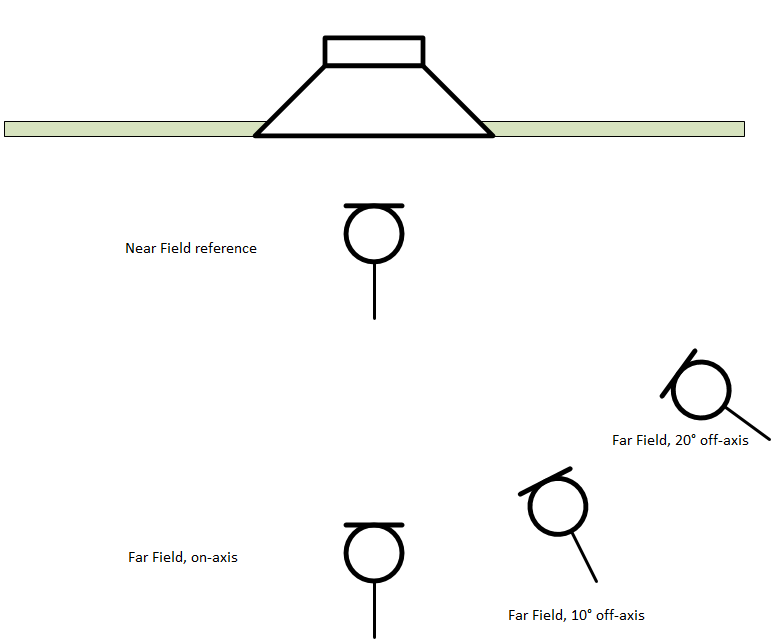
\includegraphics[width=0.7\textwidth]{RoomComp/NFFF_Setup} 
    \captionsetup{hypcap=false} 
	\captionof{figure}{Measurement setup} 
	\label{fig:SetupNFFF}
\end{center}
\end{minipage}
\begin{minipage}{0.6\textwidth}

\end{minipage}

\subsection{D. B. Keele method for Far Field extrapolation}
\todo[inline]{I don't think this subsection is very pertinent nor interesting}
D. B. Keele presented a simplified method for extrapolation of the Far Field pressure of a device by measuring in the near field. The theory is given in the article \textit{Low-Frequency Loudspeaker Assessment by Nearfield Sound-Pressure Measurement} \citep[see][]{dkeele}. The Near - Far pressure relation is given in equation \ref{eq:nfpressure}.

\begin{equation}
p_{N} = \frac{2r}{a} \cdot p_{F}
\label{eq:nfpressure}
\end{equation}
\myequations{Near-Far field pressure relation}

Where $p_{N}$ and $p_{F}$ are respectively the Near and Far field pressures, $r$ is the distance between the center of the driver's membrane and the measuring point, and $a$ the radius of the driver's membrane.\\

The results of this extrapolation, after implementation in SciLab, are given in appendix \ref{Curves:dbkFF}. 


\section{Discussion}

In this \todo[color=green]{name}{}chapter, several methods for compensating the effect of the environment on an acoustic measurement have been  investigated. 


%--------------------------------------------------------------
%	CONCLUSION
%--------------------------------------------------------------
% \chapter*{Conclusion}
% \addcontentsline{toc}{chapter}{Conclusion}

% Several investigations have been done in the context of this report and gave significant results. \\~\\

% On a more personal note, working at Klippel GmbH have been a very enjoyable experience that gives me more insight about the real functioning of a company and what to expect from my future. I am thrilled to have had the opportunity to conduct this work, and very satisfied with the variety of the tasks I was assigned to, which included programming, measuring, and research to draw conclusion from my experiments. \\

% Thank you for reading my work.

%--------------------------------------------------------------
%	BIBLIOGRAPHY
%--------------------------------------------------------------

\bibliography{bibli}
\bibliographystyle{abbrv}

\nocite{*}

%--------------------------------------------------------------
%	APPENDIX
%--------------------------------------------------------------

\begin{appendices}

		% Additional curves
\chapter{Additional figures}
This appendix aims to present additional figures that could not be presented in the corpus of this report because of their size, or lacked of relevancy for the discussions. To simplify the navigation, the titles of the section will be the same as the tittle of the chapters this figures are complemented with. 


\section{Baffle measurement}
\subsection{Estimation of baffle influence}
\label{Curves:BaffleInfluence}

\begin{center}
	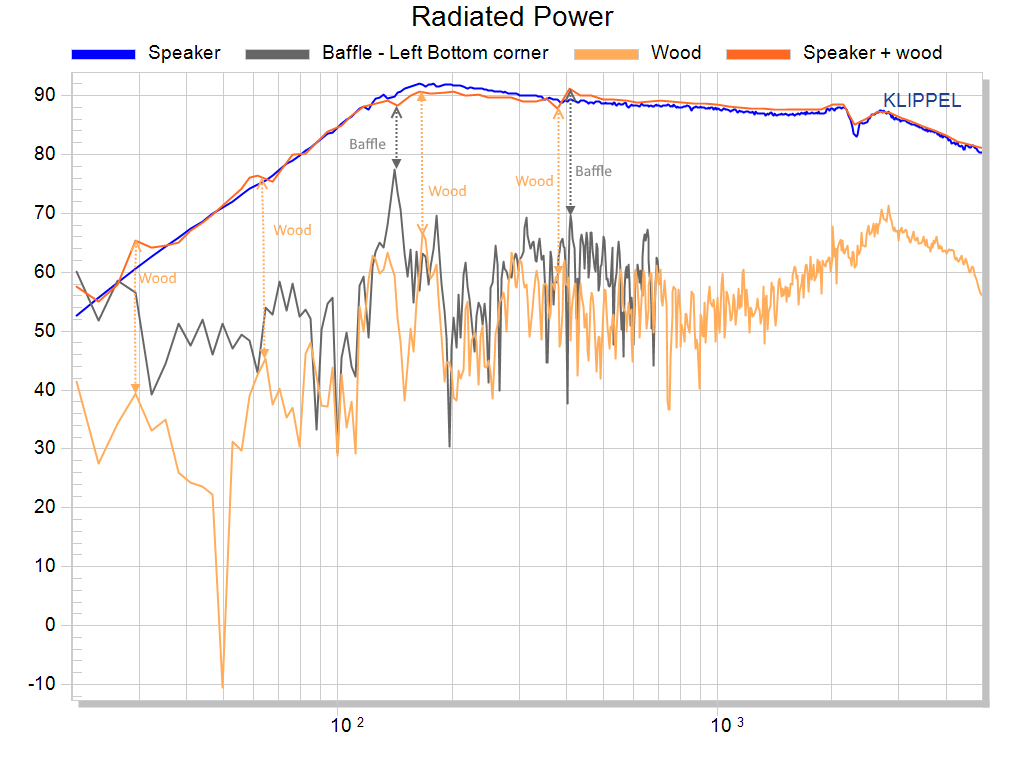
\includegraphics[width=0.9\textwidth]{Appendix/Vib_RadPow}
    \captionsetup{hypcap=false}
    \captionof{figure}{Radiated Powers at 1m for different measurement points on the baffle}
    \label{Curves:Baffle_RadPow}
\end{center}


\section{Measurement time optimization}

\subsection{10 cm woofer}
\label{Curves:10cm}

\begin{minipage}{0.5\textwidth}
\begin{center}
	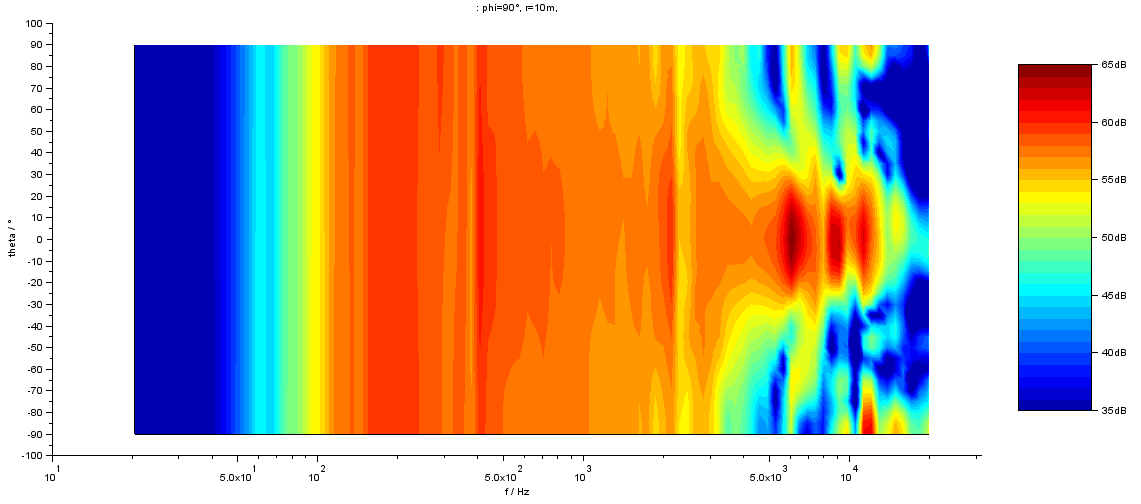
\includegraphics[width=.9\textwidth]{Sym/contour} 
    \captionsetup{hypcap=false} 
	\captionof{figure}{Contour plot of the woofer at 10 m, centered on-axis, horizontal plane.} 
	\label{fig:contour_10cm}
\end{center}
\end{minipage}
\begin{minipage}{0.5\textwidth}
\begin{center}
	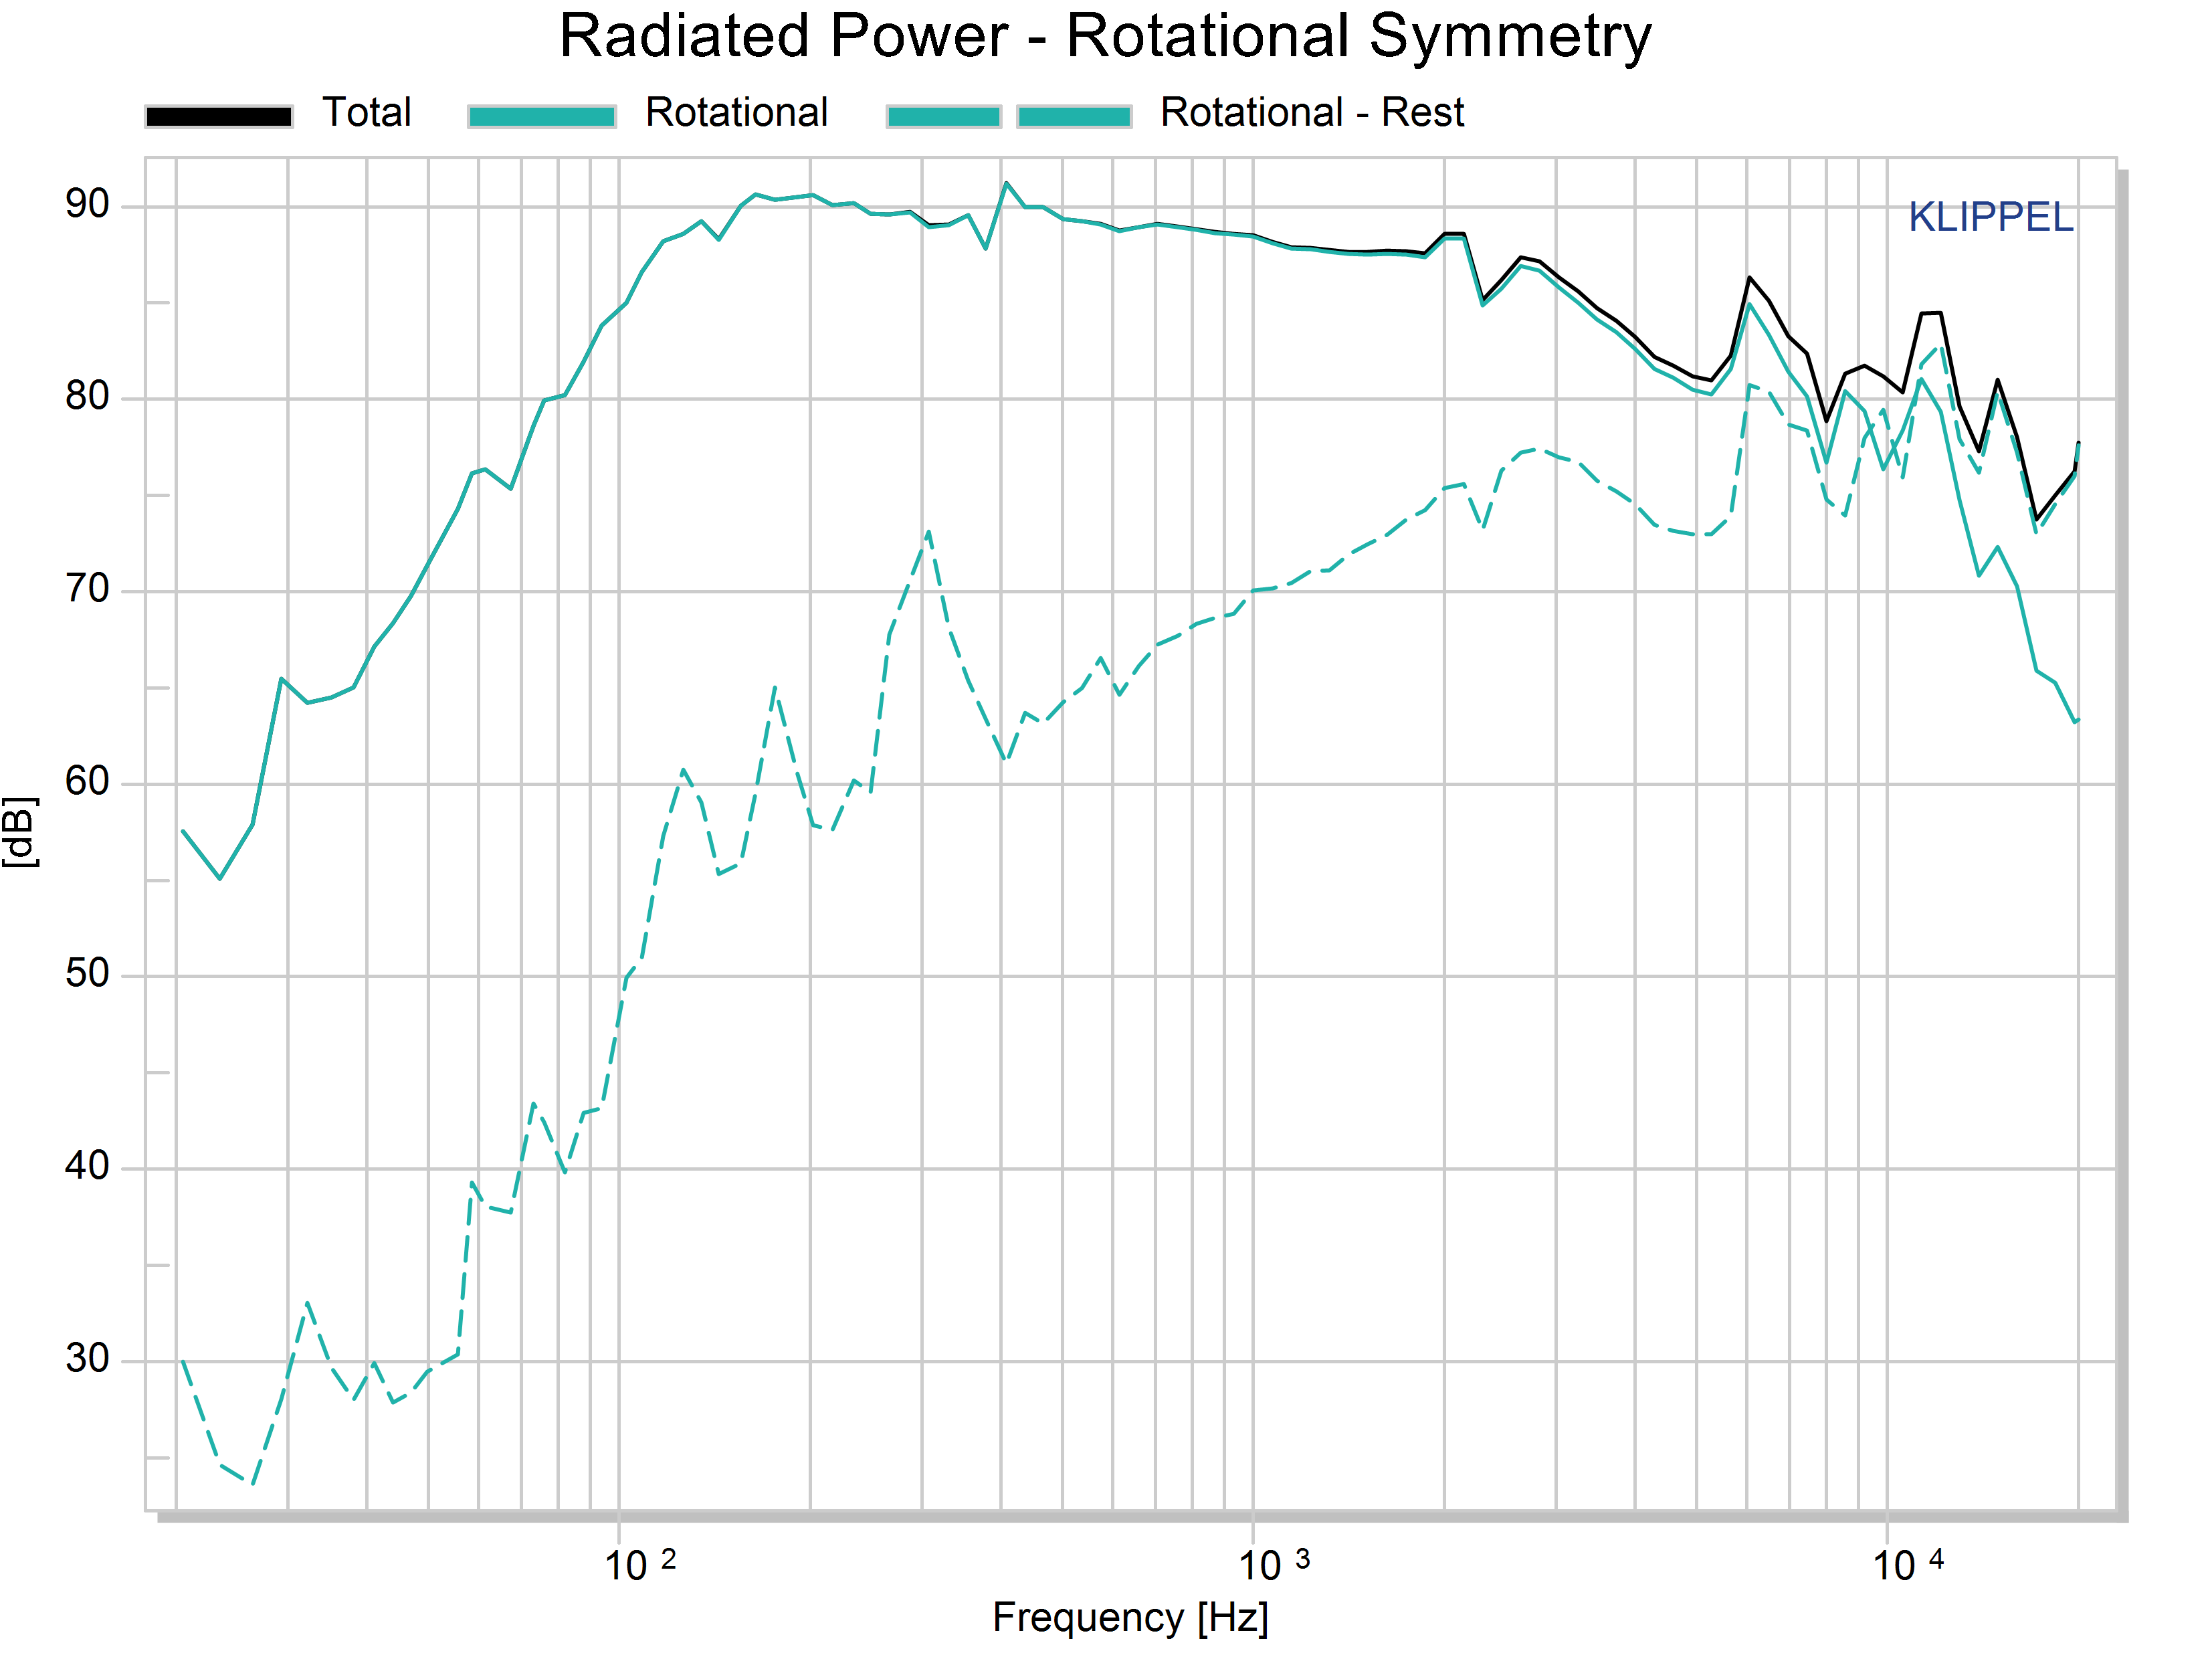
\includegraphics[width=0.9\textwidth]{Sym/10cm_RadPow_Rot}
    \captionsetup{hypcap=false}
    \captionof{figure}{10 cm woofer, Radiated Powers: rotational symmetry}
\end{center}
\end{minipage}

\begin{minipage}{0.5\textwidth}
\begin{center}
	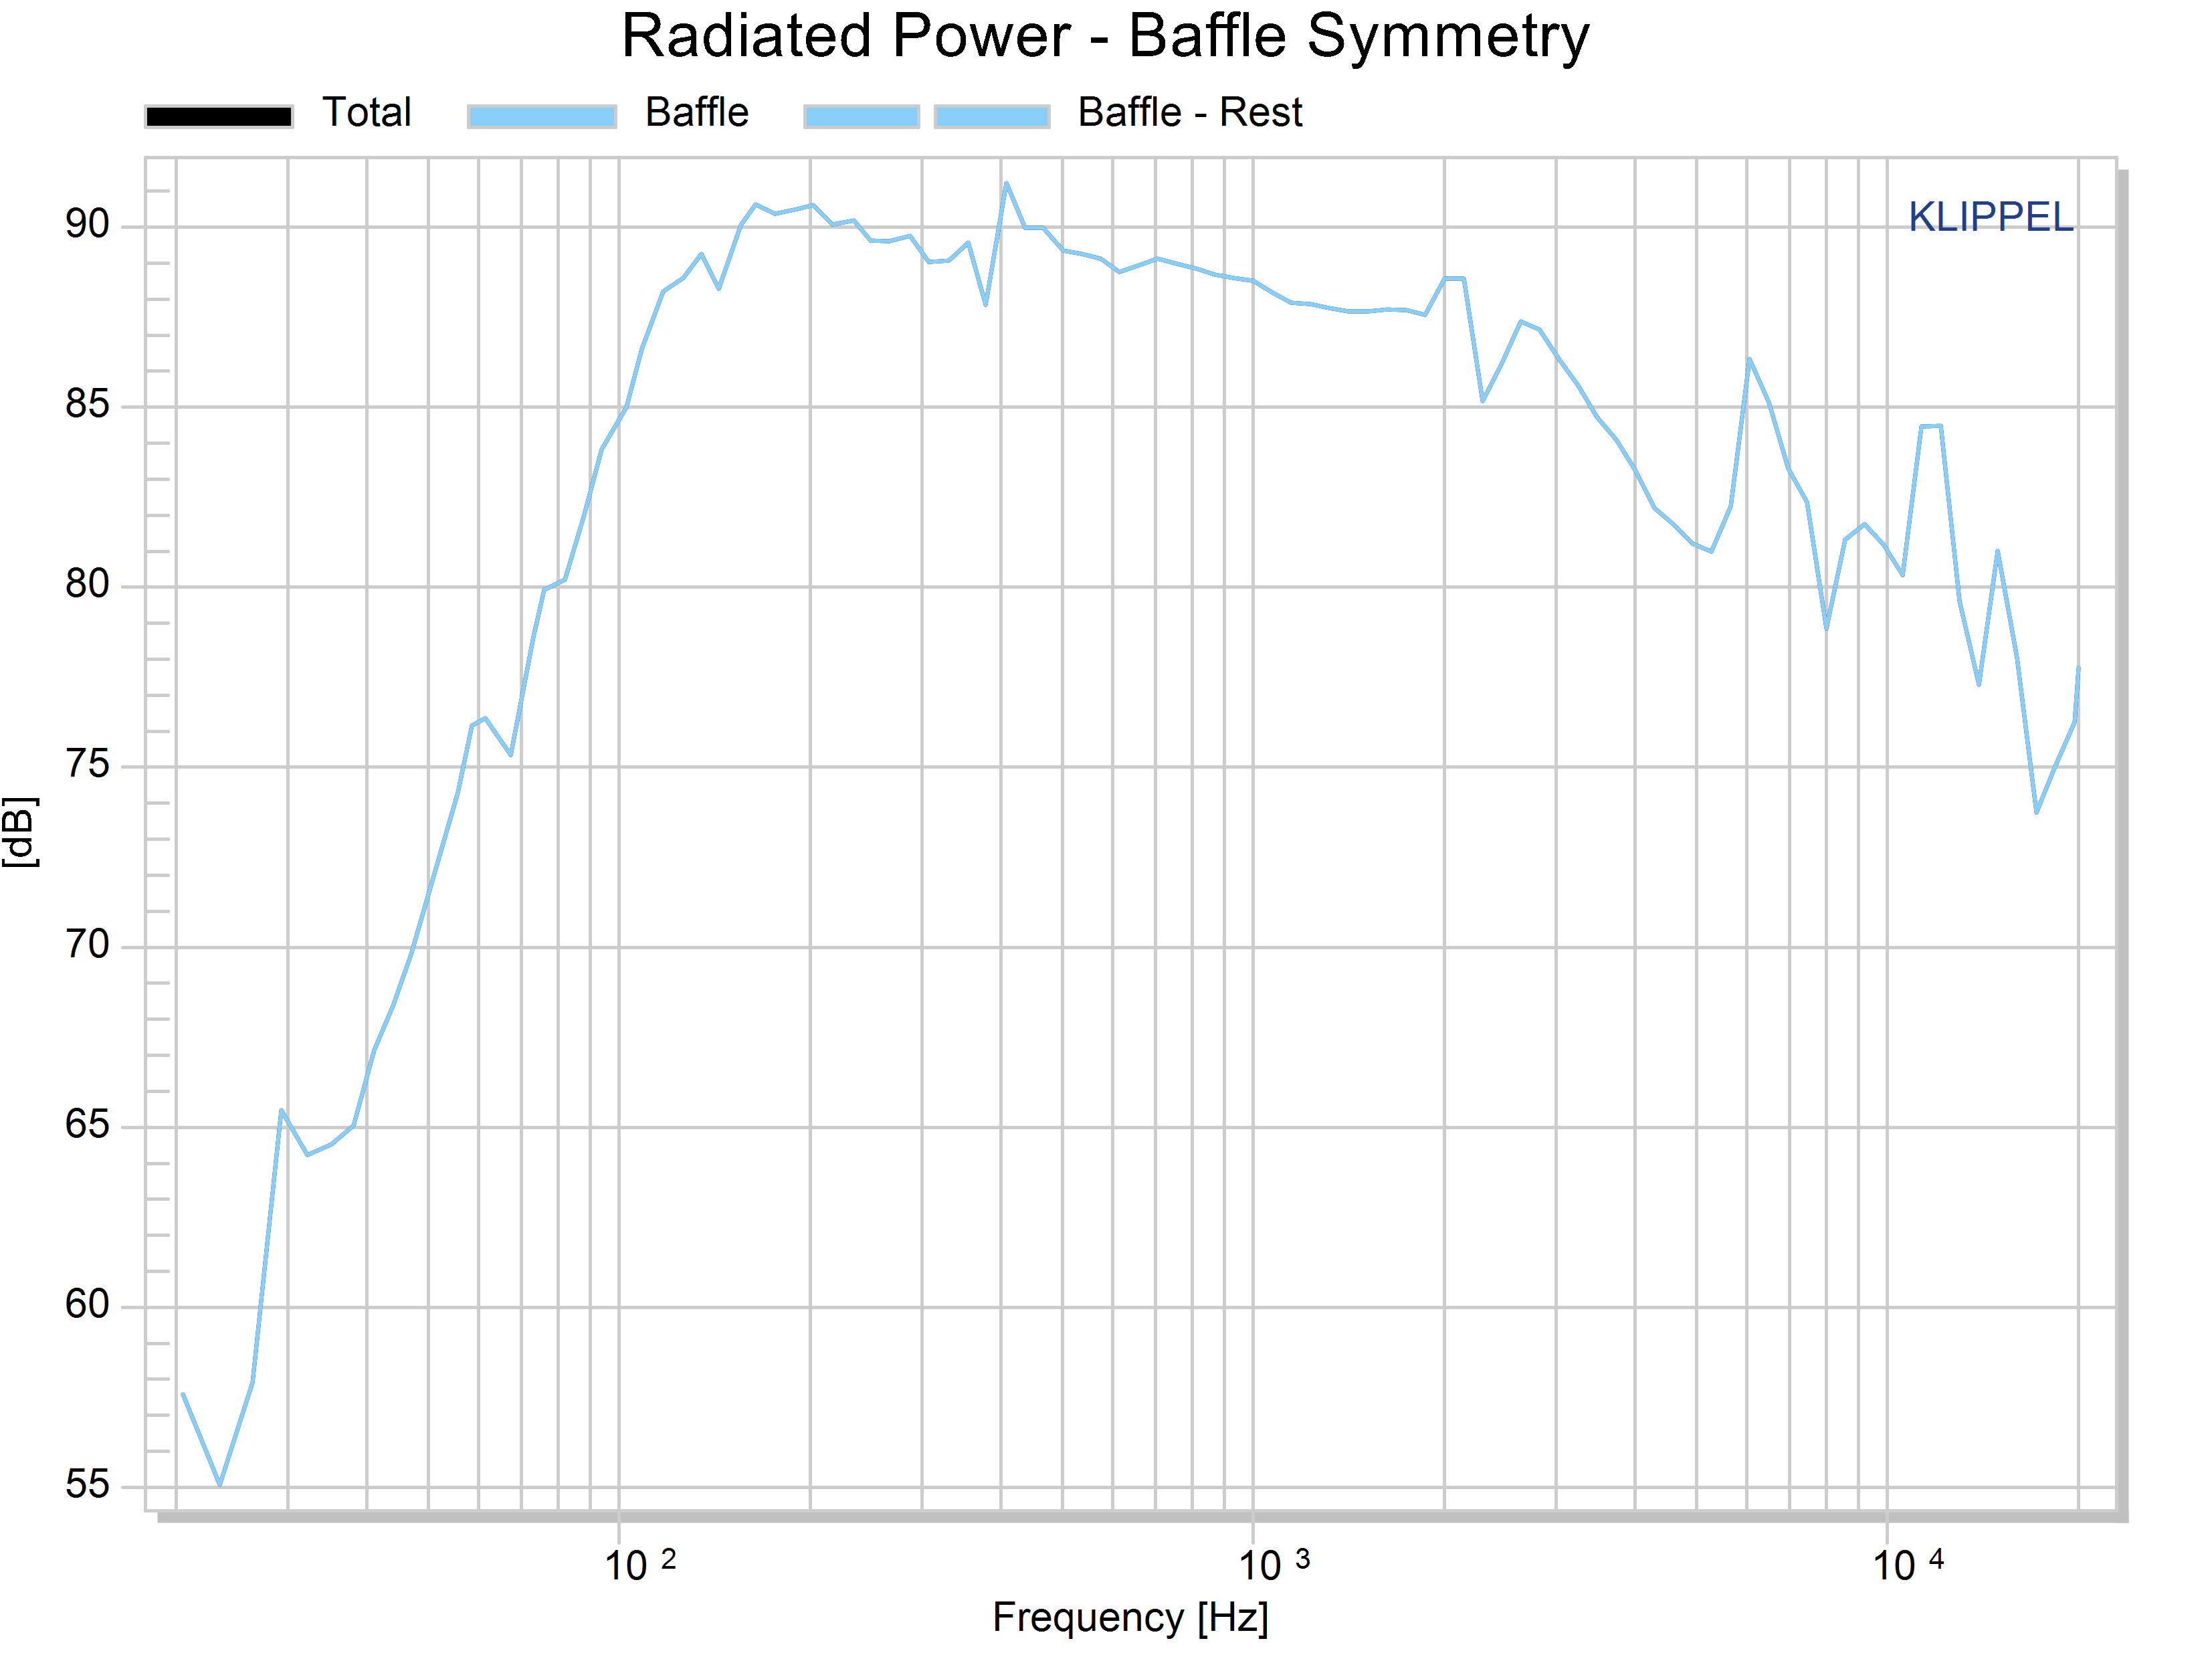
\includegraphics[width=0.9\textwidth]{Sym/10cm_RadPow_B}
    \captionsetup{hypcap=false}
    \captionof{figure}{10 cm woofer, Radiated Powers: baffle symmetry}
\end{center}
\end{minipage}
\begin{minipage}{0.5\textwidth}
\begin{center}
	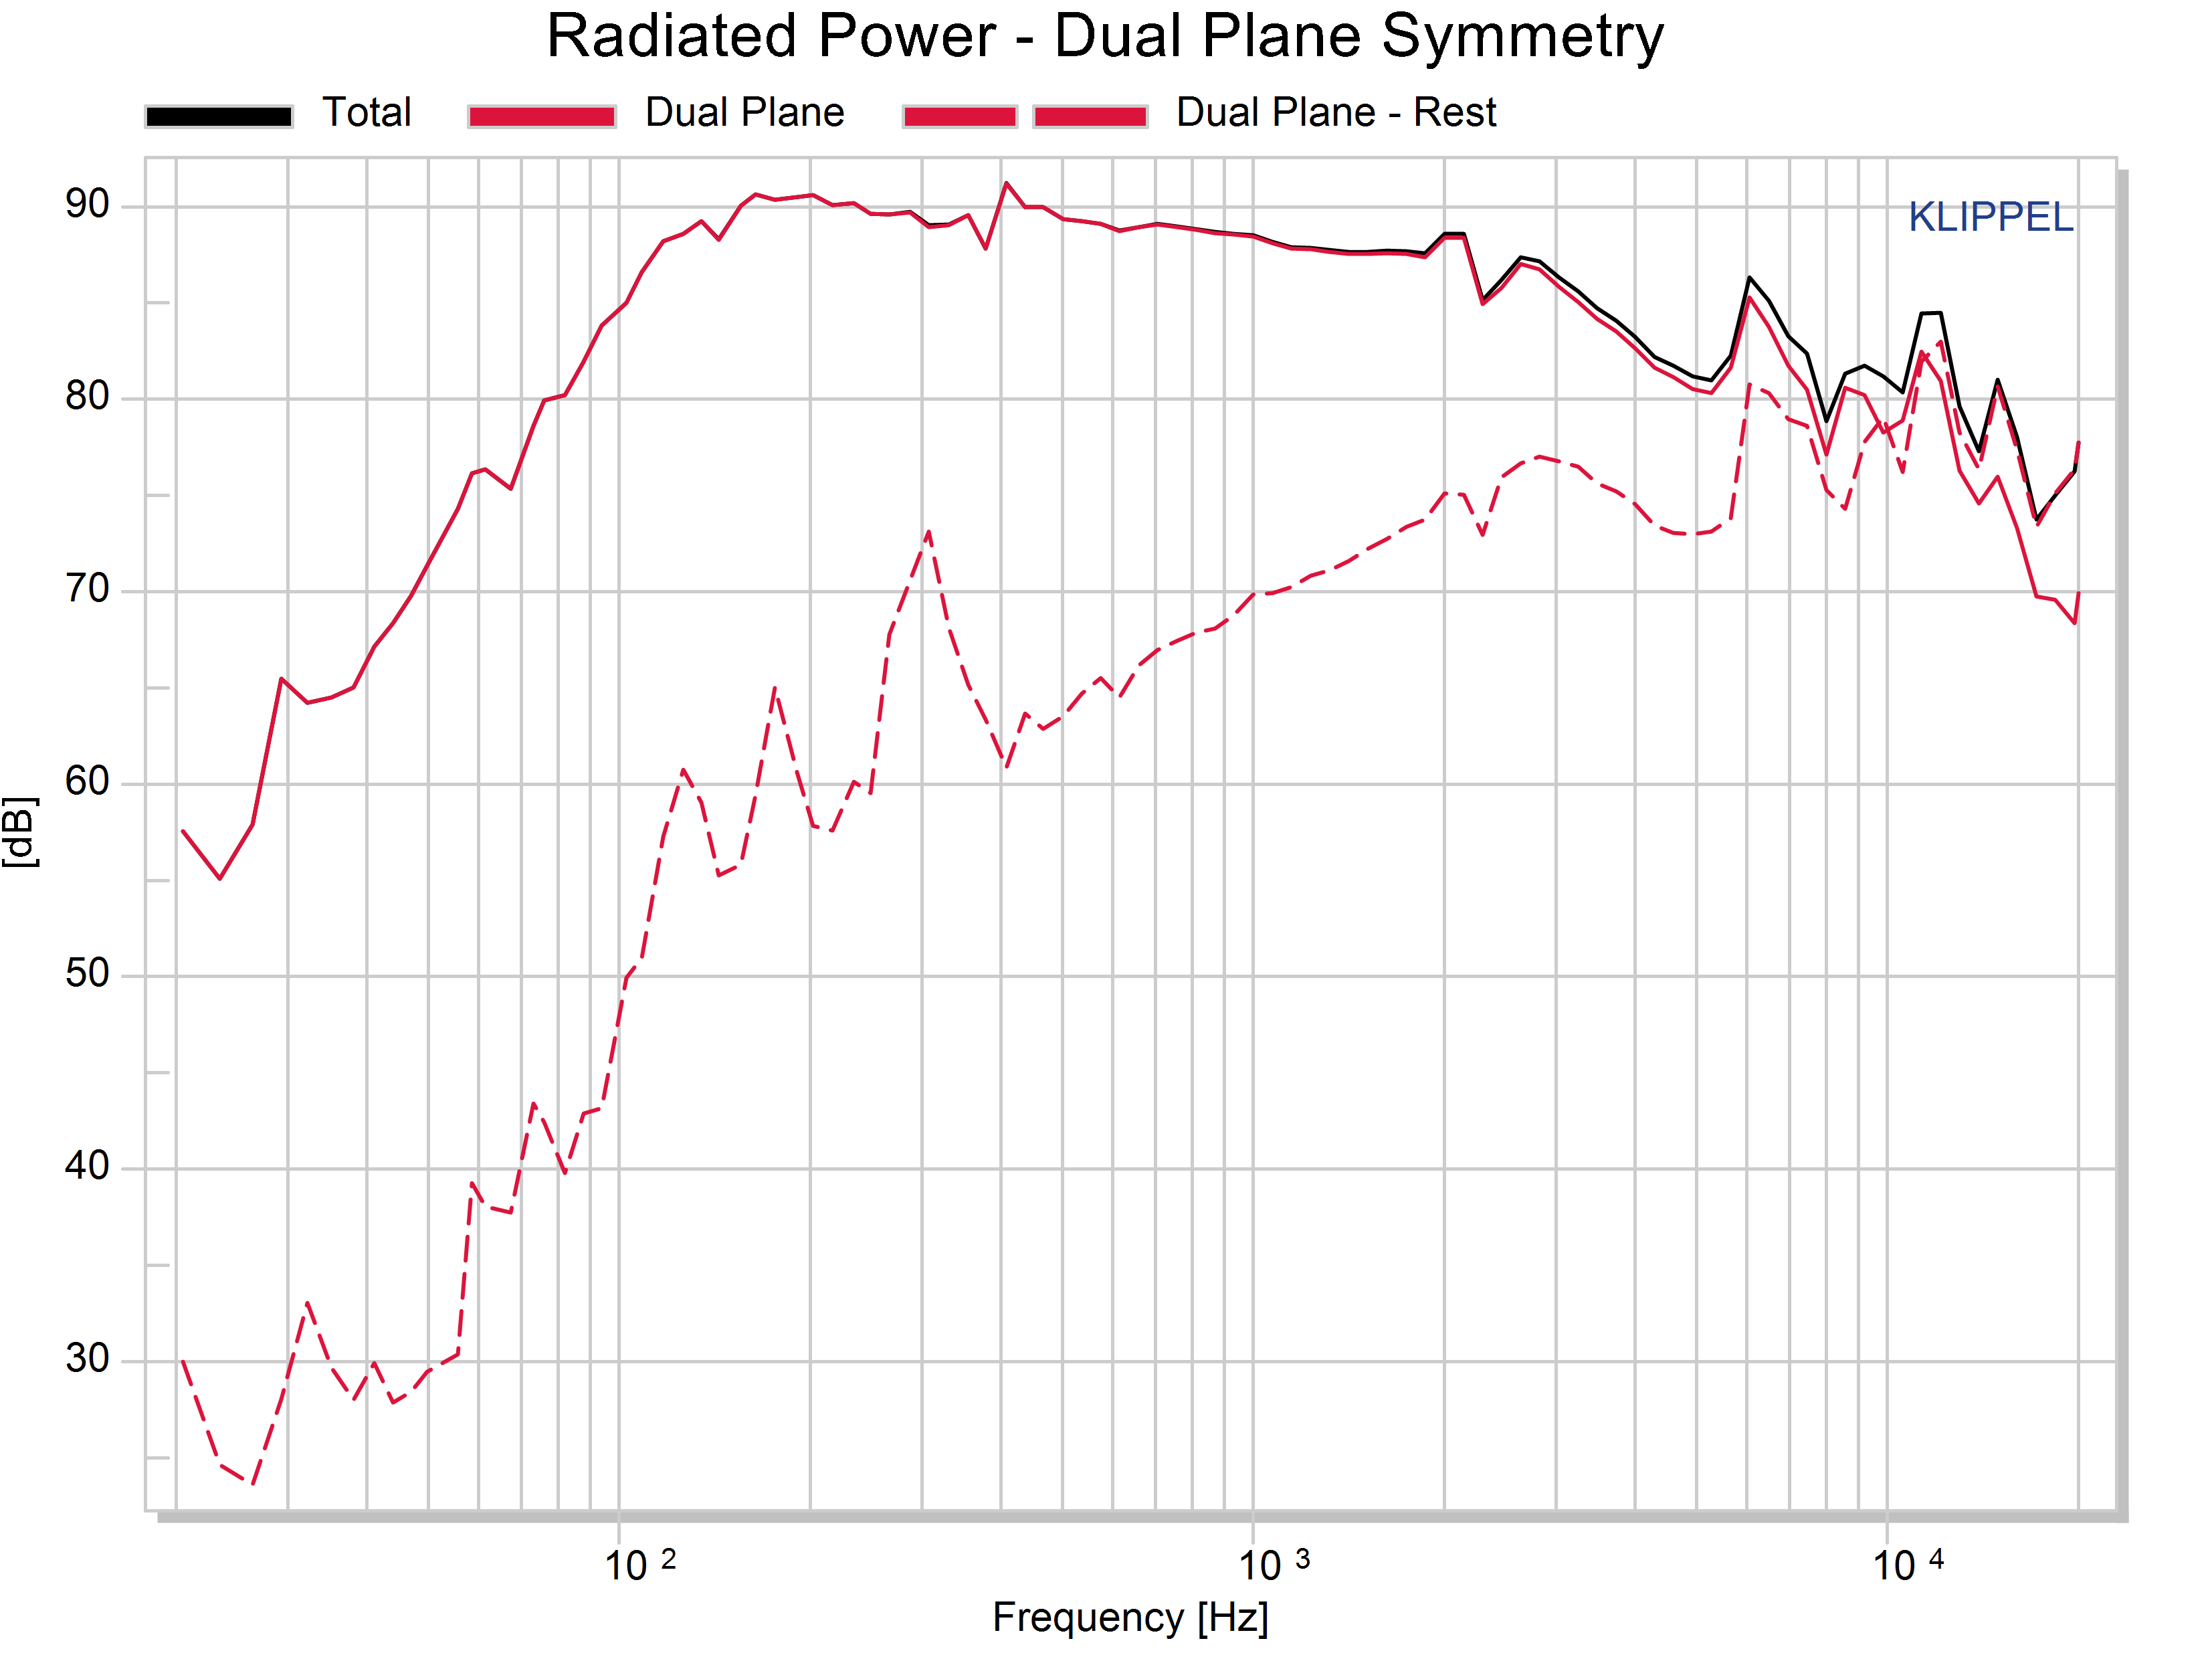
\includegraphics[width=0.9\textwidth]{Sym/10cm_RadPow_Dps}
    \captionsetup{hypcap=false}
    \captionof{figure}{10 cm woofer, Radiated Powers: dual plane symmetry}
\end{center}
\end{minipage}

\begin{minipage}{0.5\textwidth}
\begin{center}
	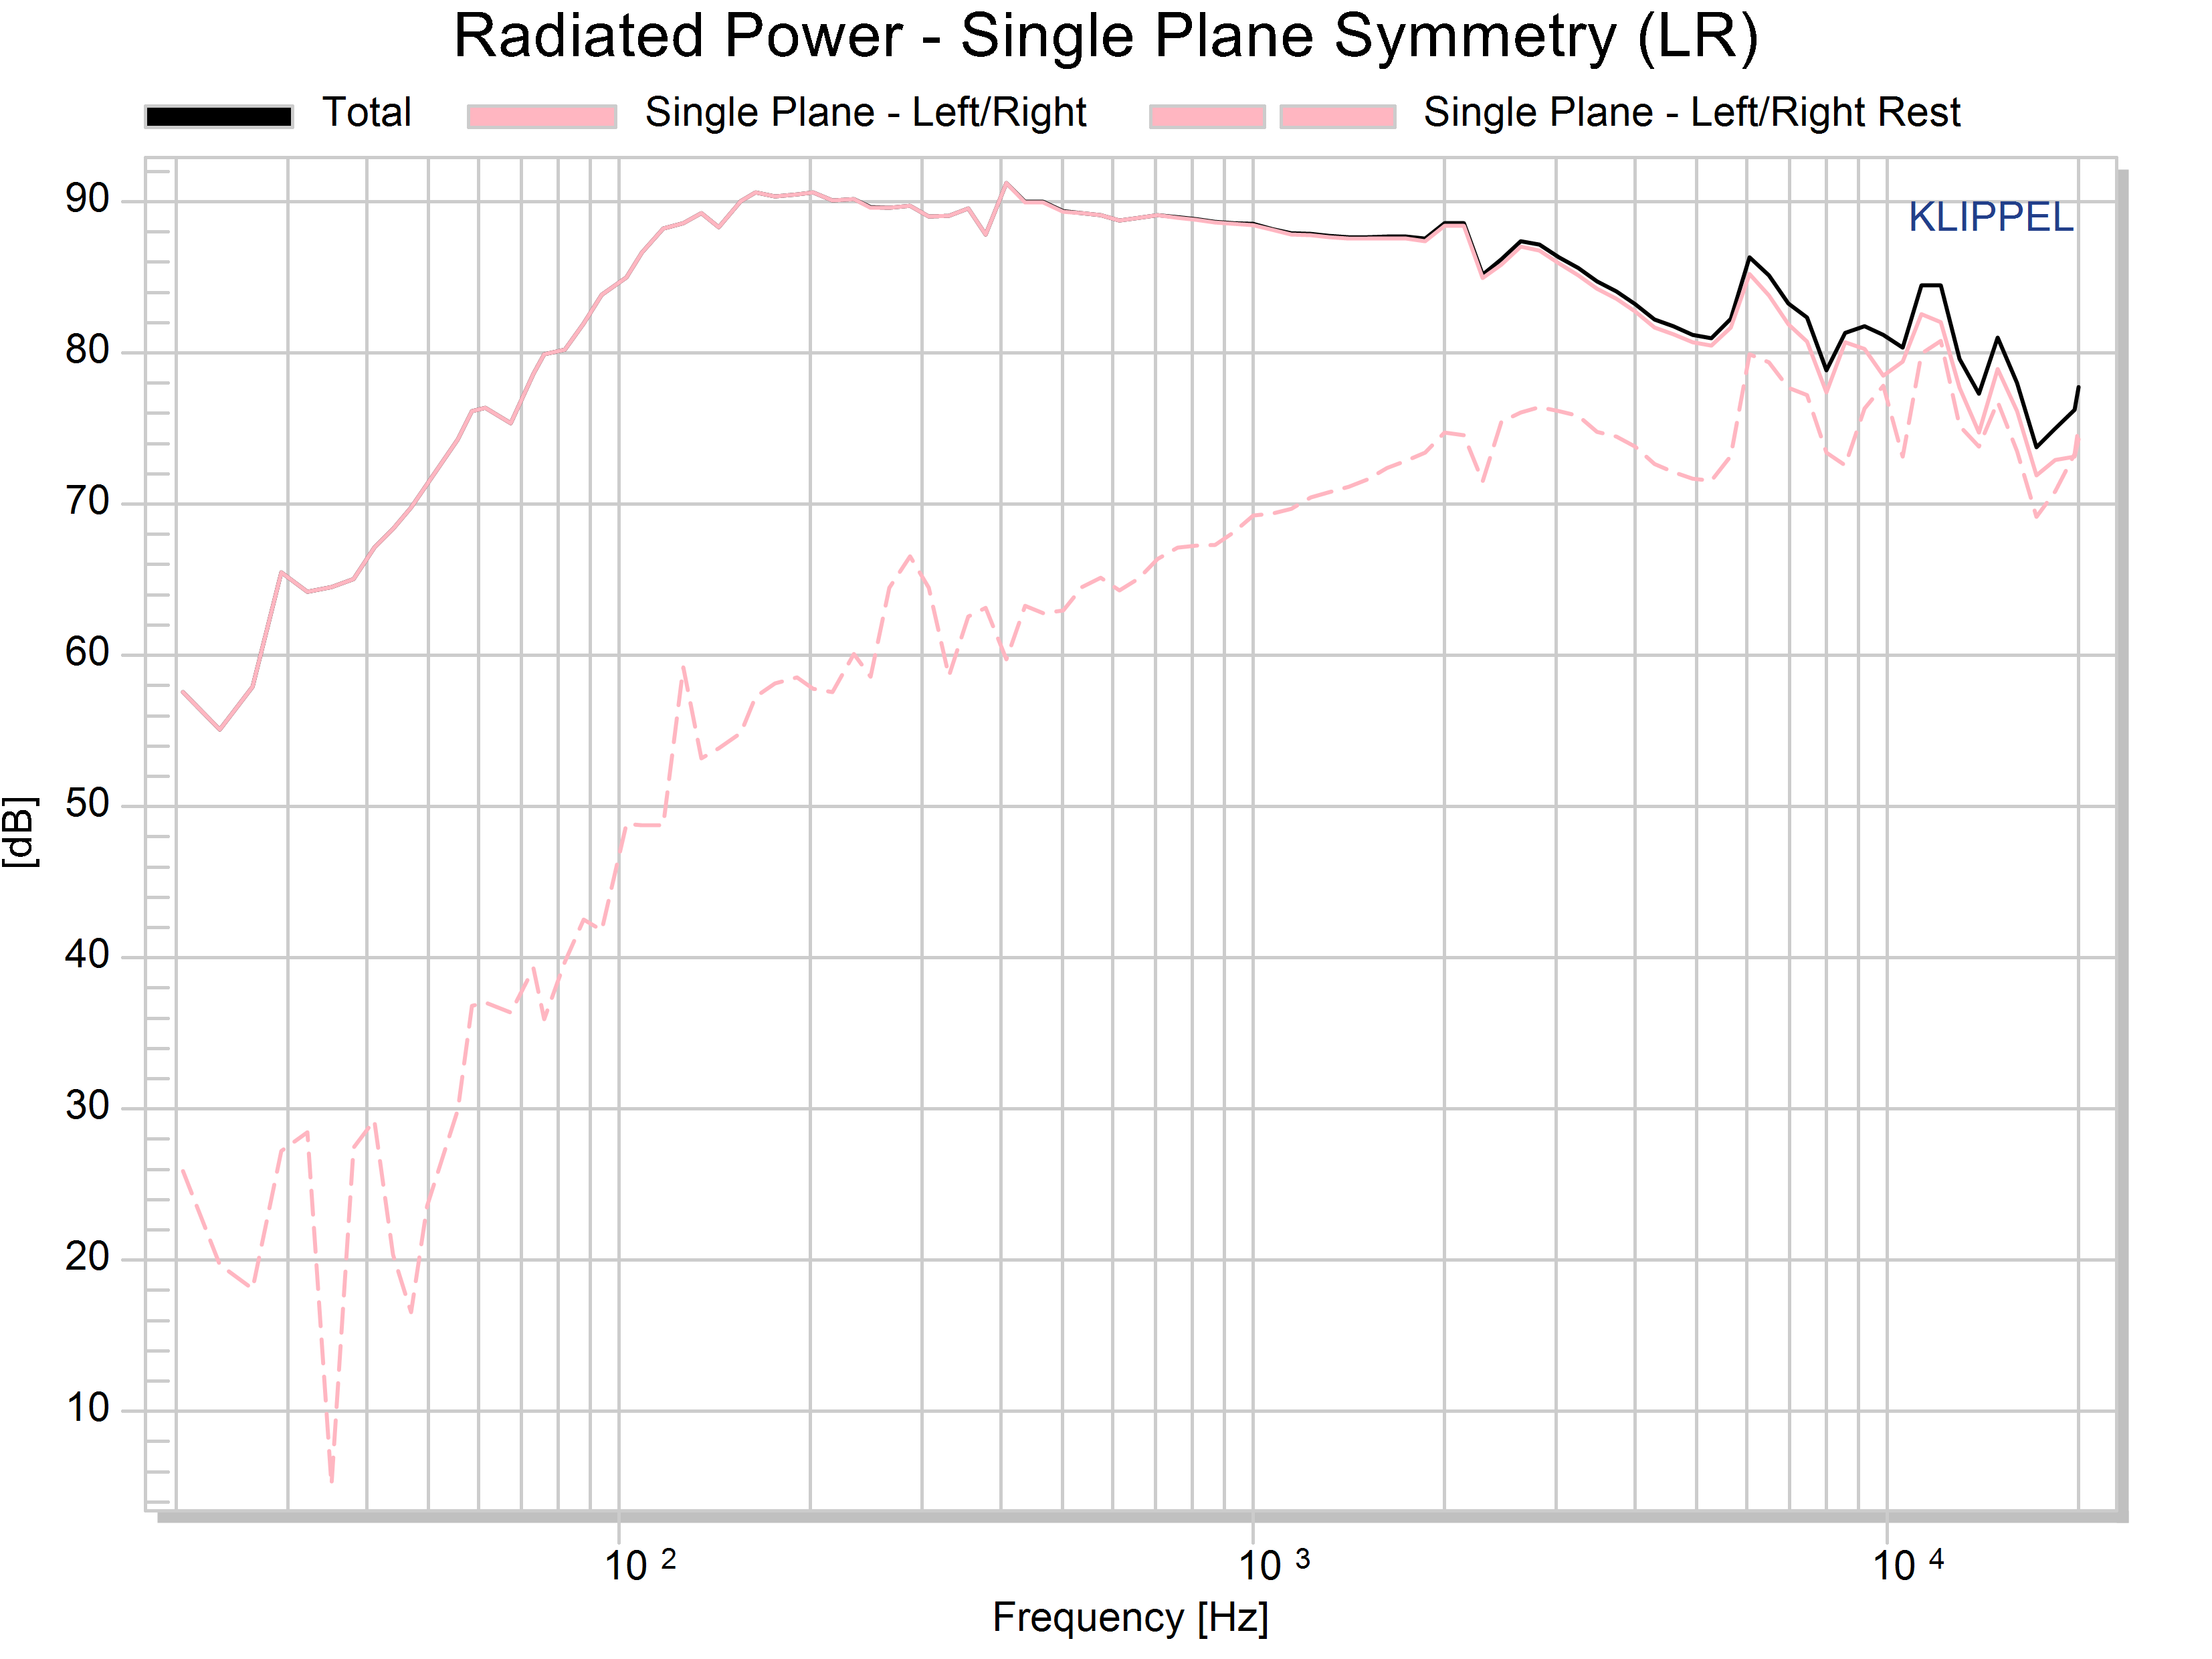
\includegraphics[width=0.9\textwidth]{Sym/10cm_RadPow_SpsLR}
    \captionsetup{hypcap=false}
    \captionof{figure}{10 cm woofer, Radiated Powers: single plane (left/right) symmetry}
\end{center}
\end{minipage}
\begin{minipage}{0.5\textwidth}
\begin{center}
	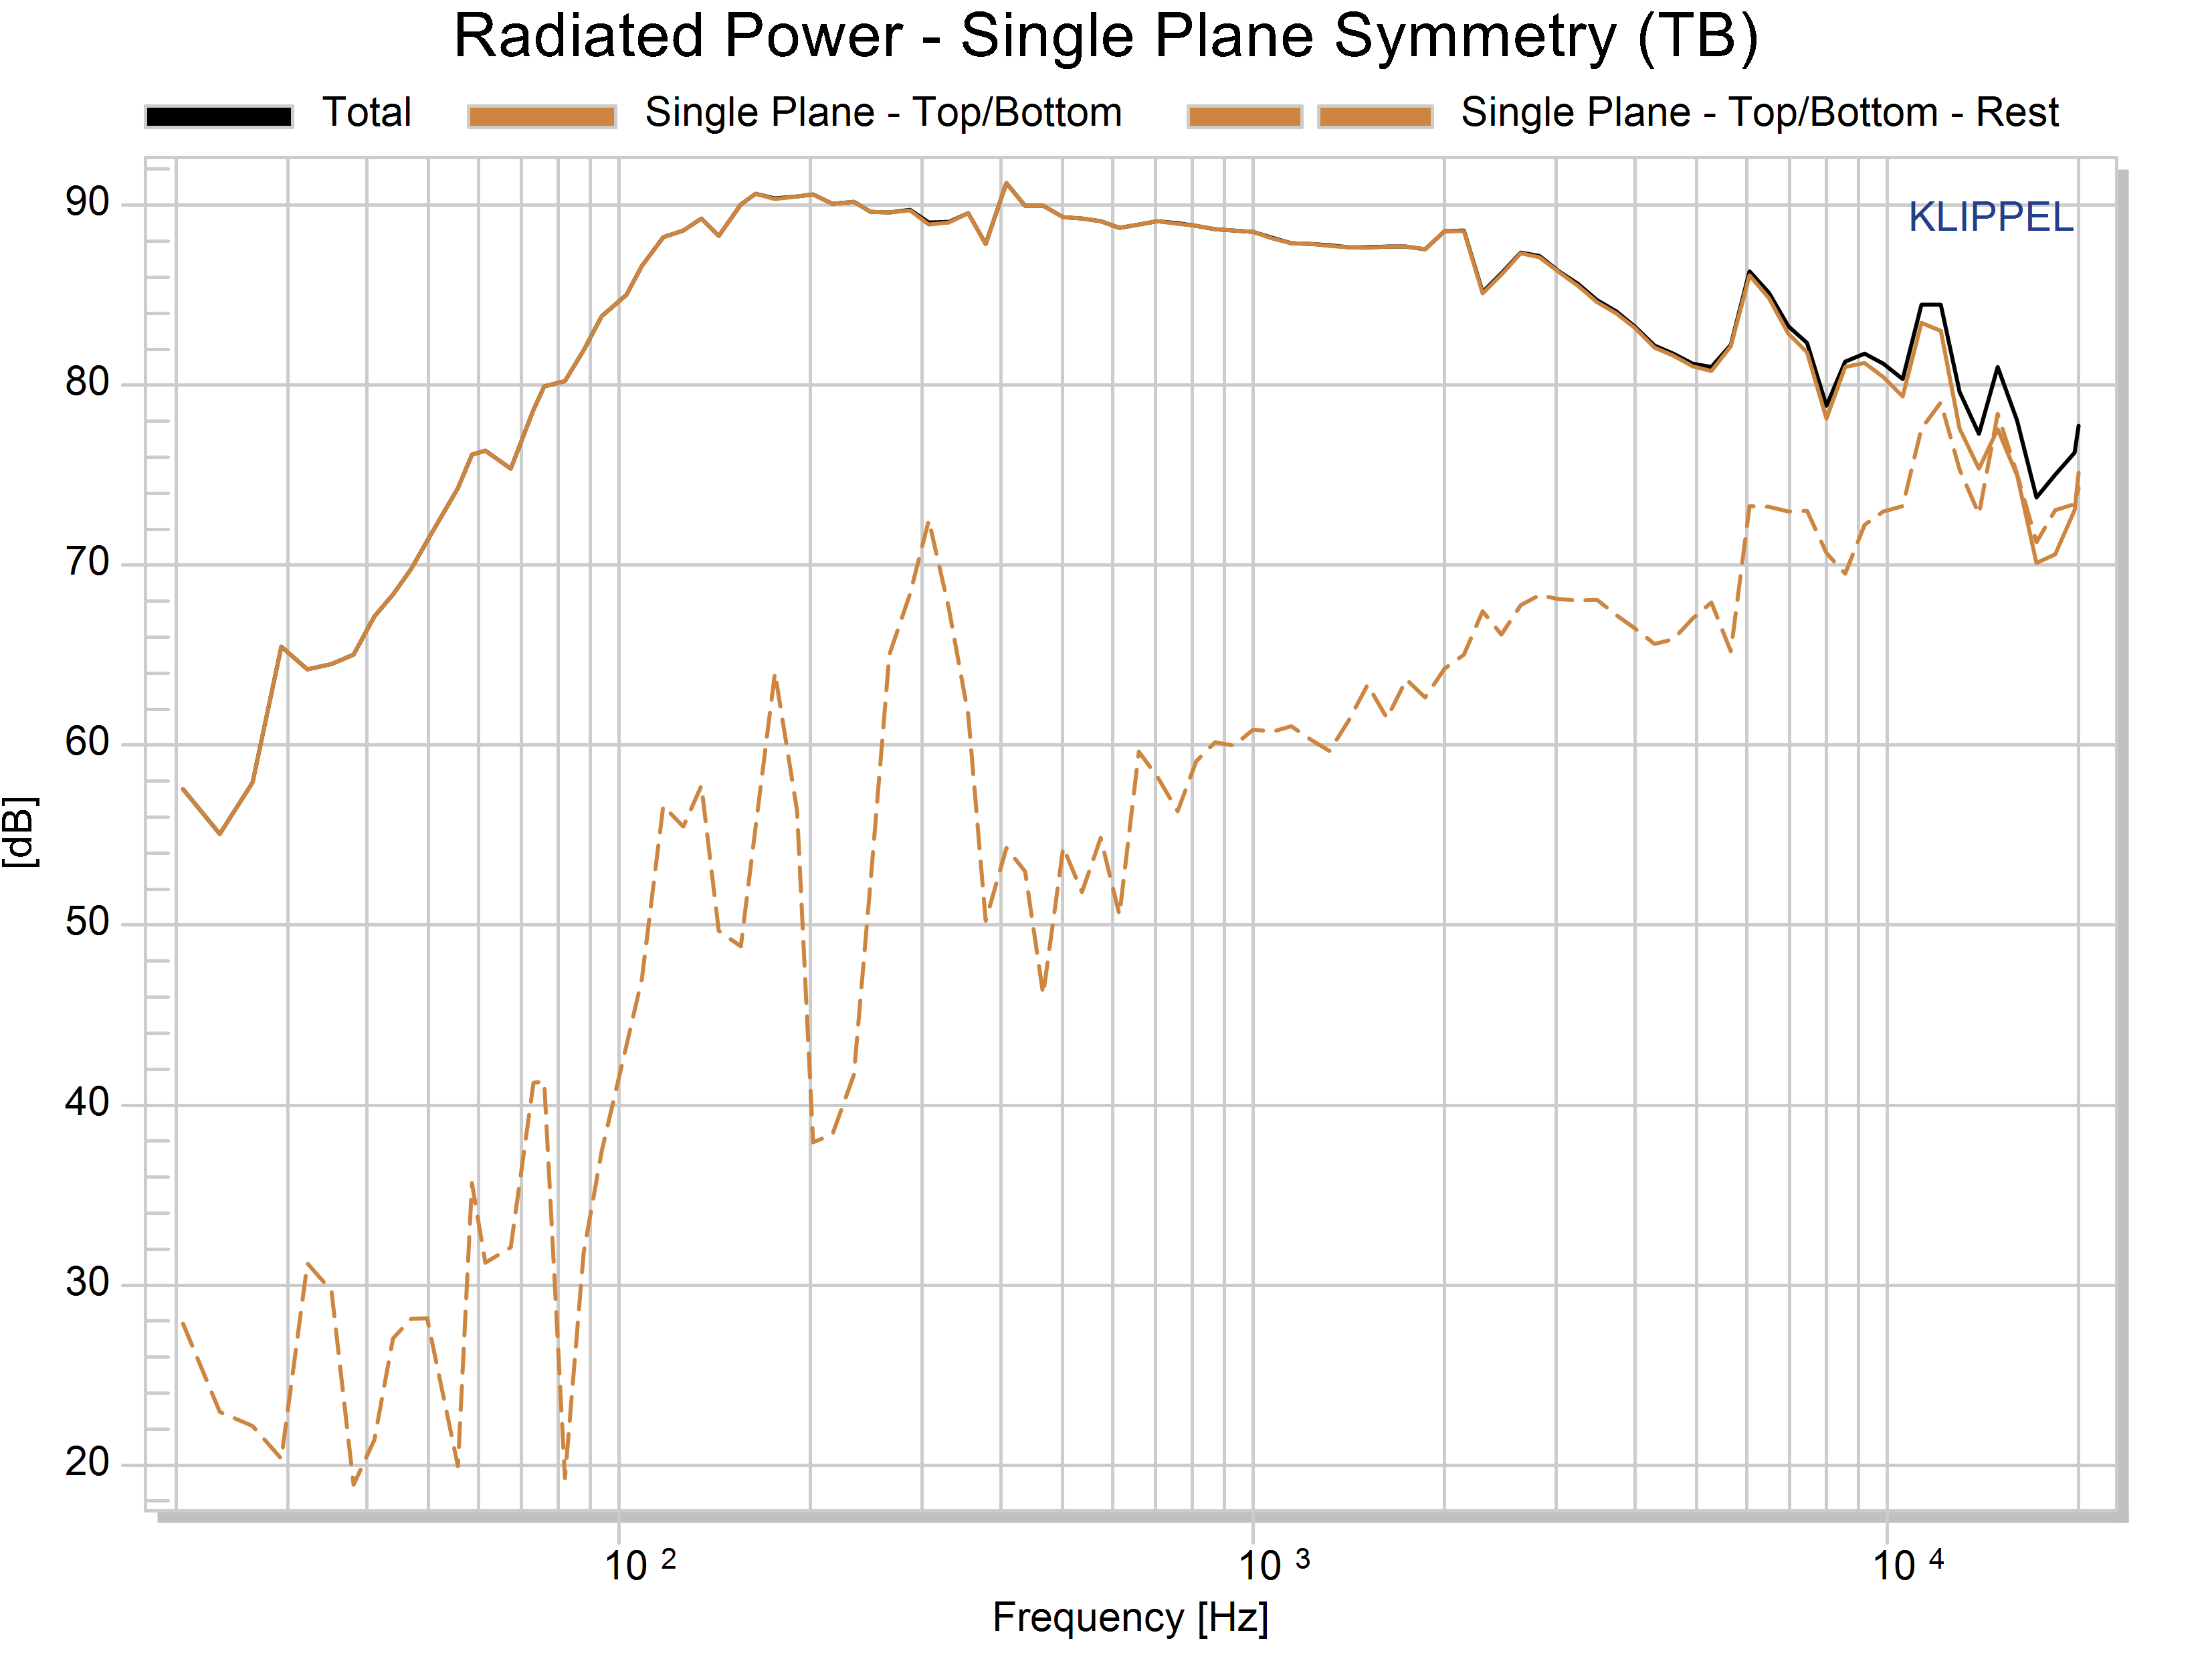
\includegraphics[width=0.9\textwidth]{Sym/10cm_RadPow_SpsTB}
    \captionsetup{hypcap=false}
    \captionof{figure}{10 cm woofer, Radiated Powers: single plane (top/bottom) symmetry}
\end{center}
\end{minipage}

\subsection{Oval speaker}
\label{Curves:oval}

\begin{minipage}{0.5\textwidth}
\begin{center}
	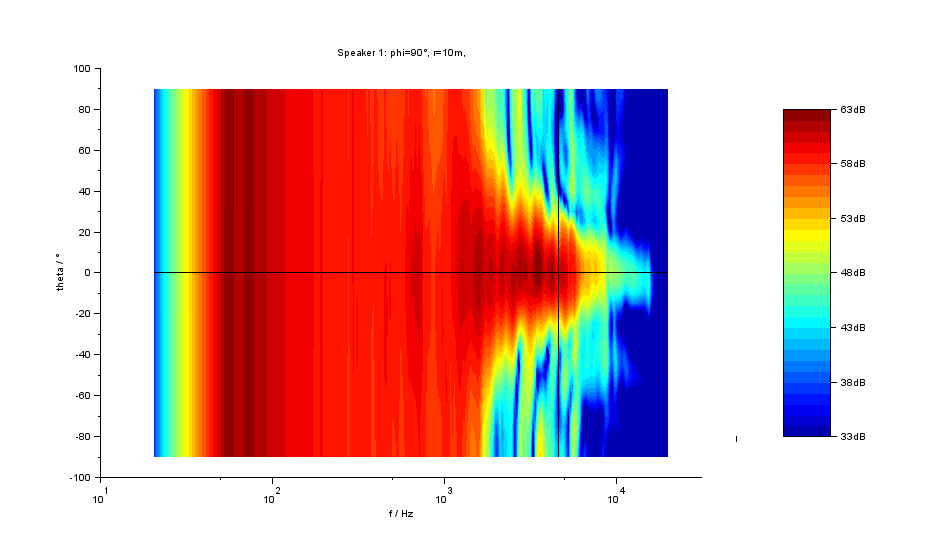
\includegraphics[width=\textwidth]{Sym/contour_oval}
    \captionsetup{hypcap=false}
    \captionof{figure}{Oval speaker, Radiated Powers: zoom on 6 - 20 kHz}
    \label{Curves:oval_contour}
\end{center}
\end{minipage}
\begin{minipage}{0.5\textwidth}
\begin{center}
	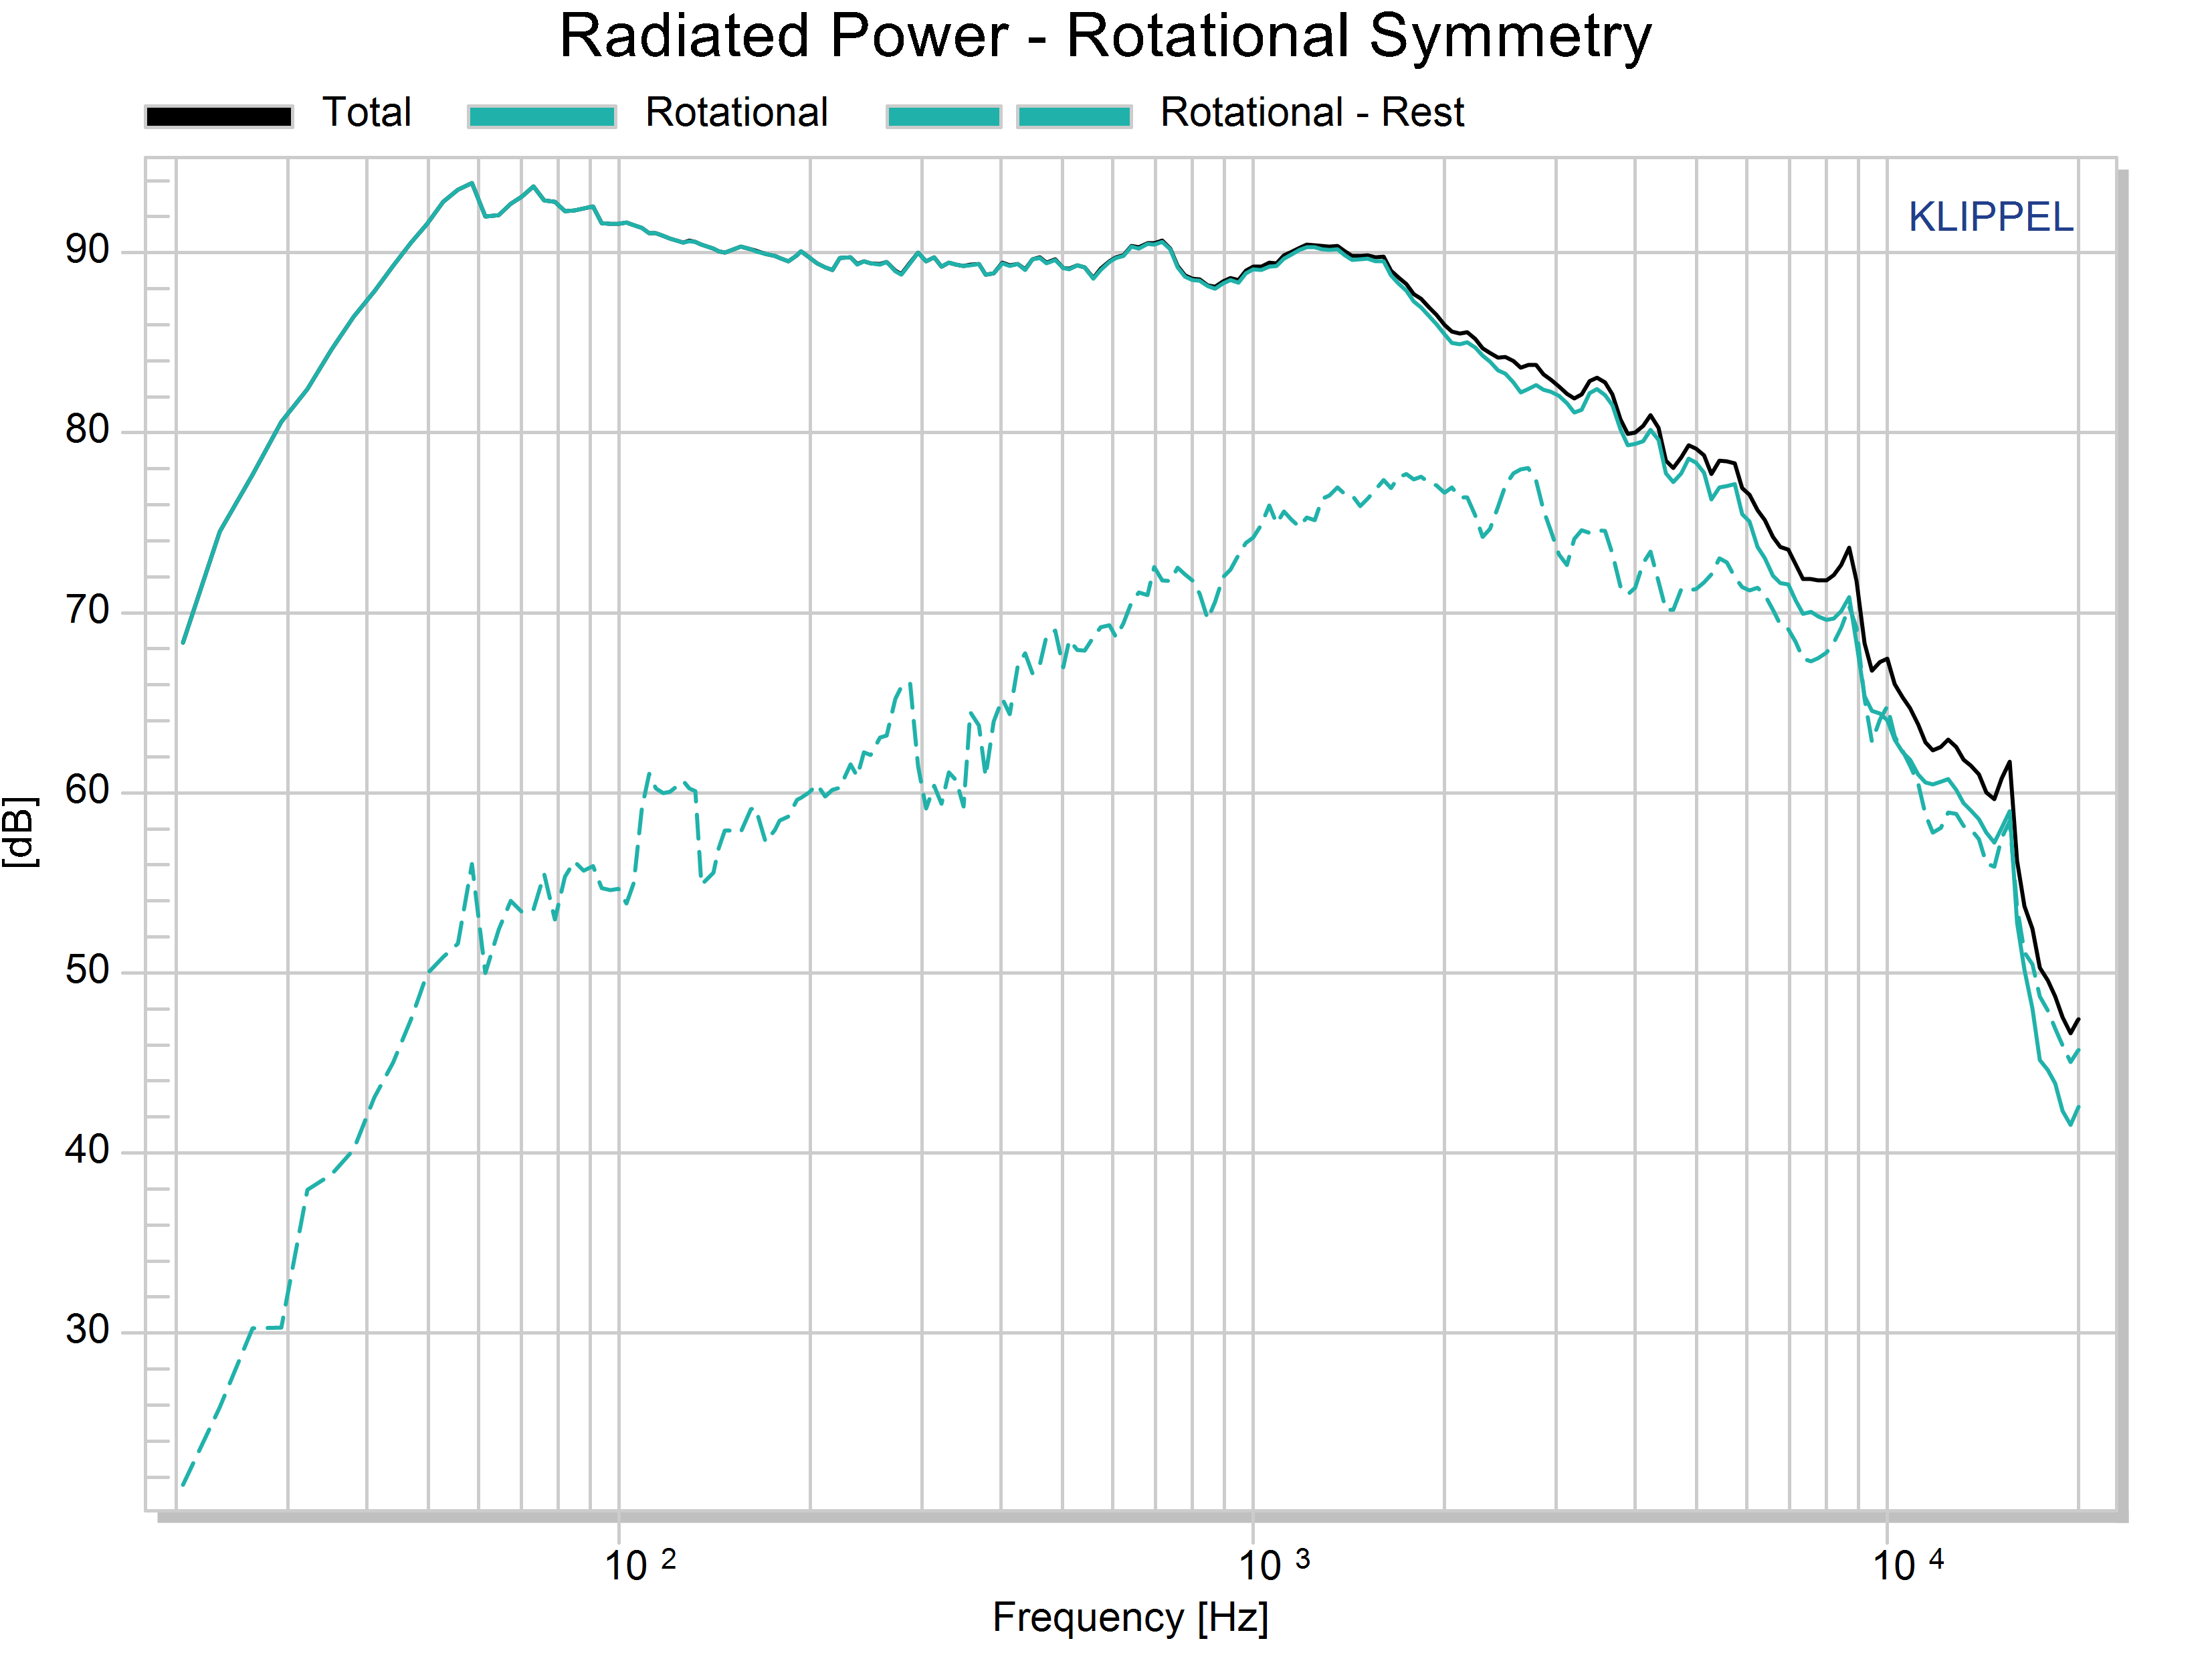
\includegraphics[width=0.9\textwidth]{Sym/Oval_RadPow_Rot}
    \captionsetup{hypcap=false}
    \captionof{figure}{Oval speaker, Radiated Powers: rotational symmetry}
\end{center}
\end{minipage}

\begin{minipage}{0.5\textwidth}
\begin{center}
	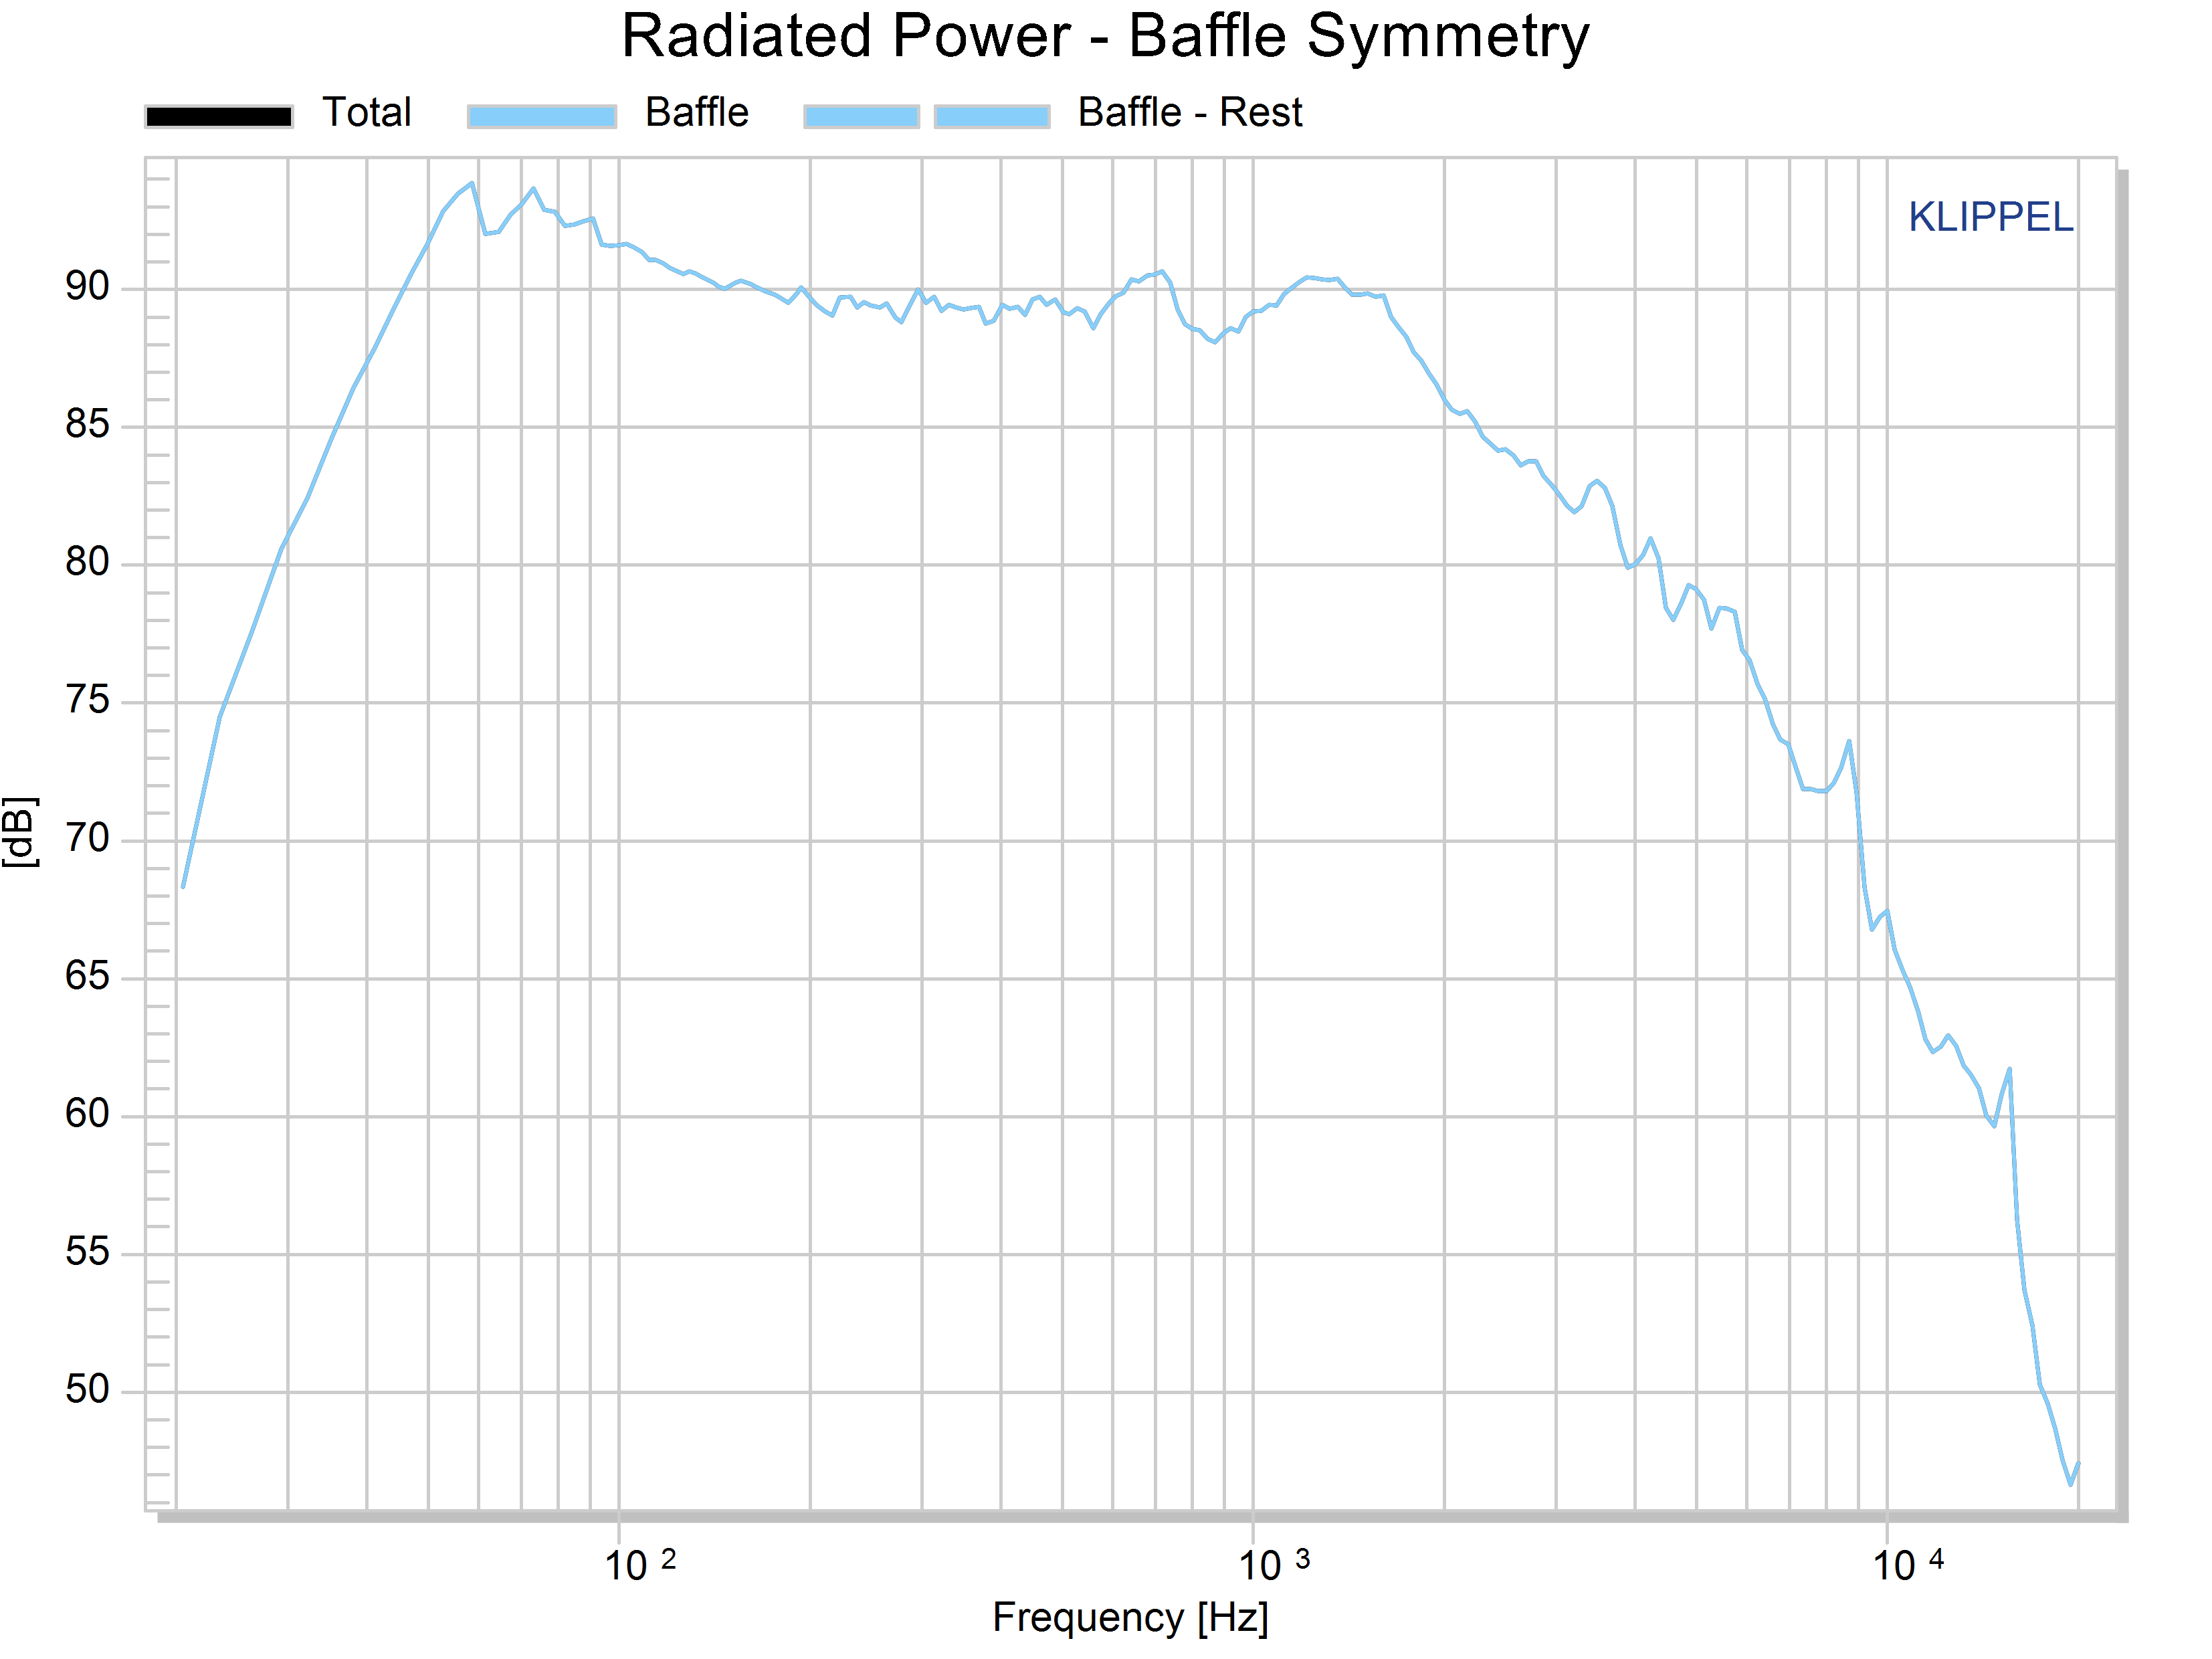
\includegraphics[width=0.9\textwidth]{Sym/Oval_RadPow_B}
    \captionsetup{hypcap=false}
    \captionof{figure}{Oval speaker, Radiated Powers: baffle symmetry}
\end{center}
\end{minipage}
\begin{minipage}{0.5\textwidth}
\begin{center}
	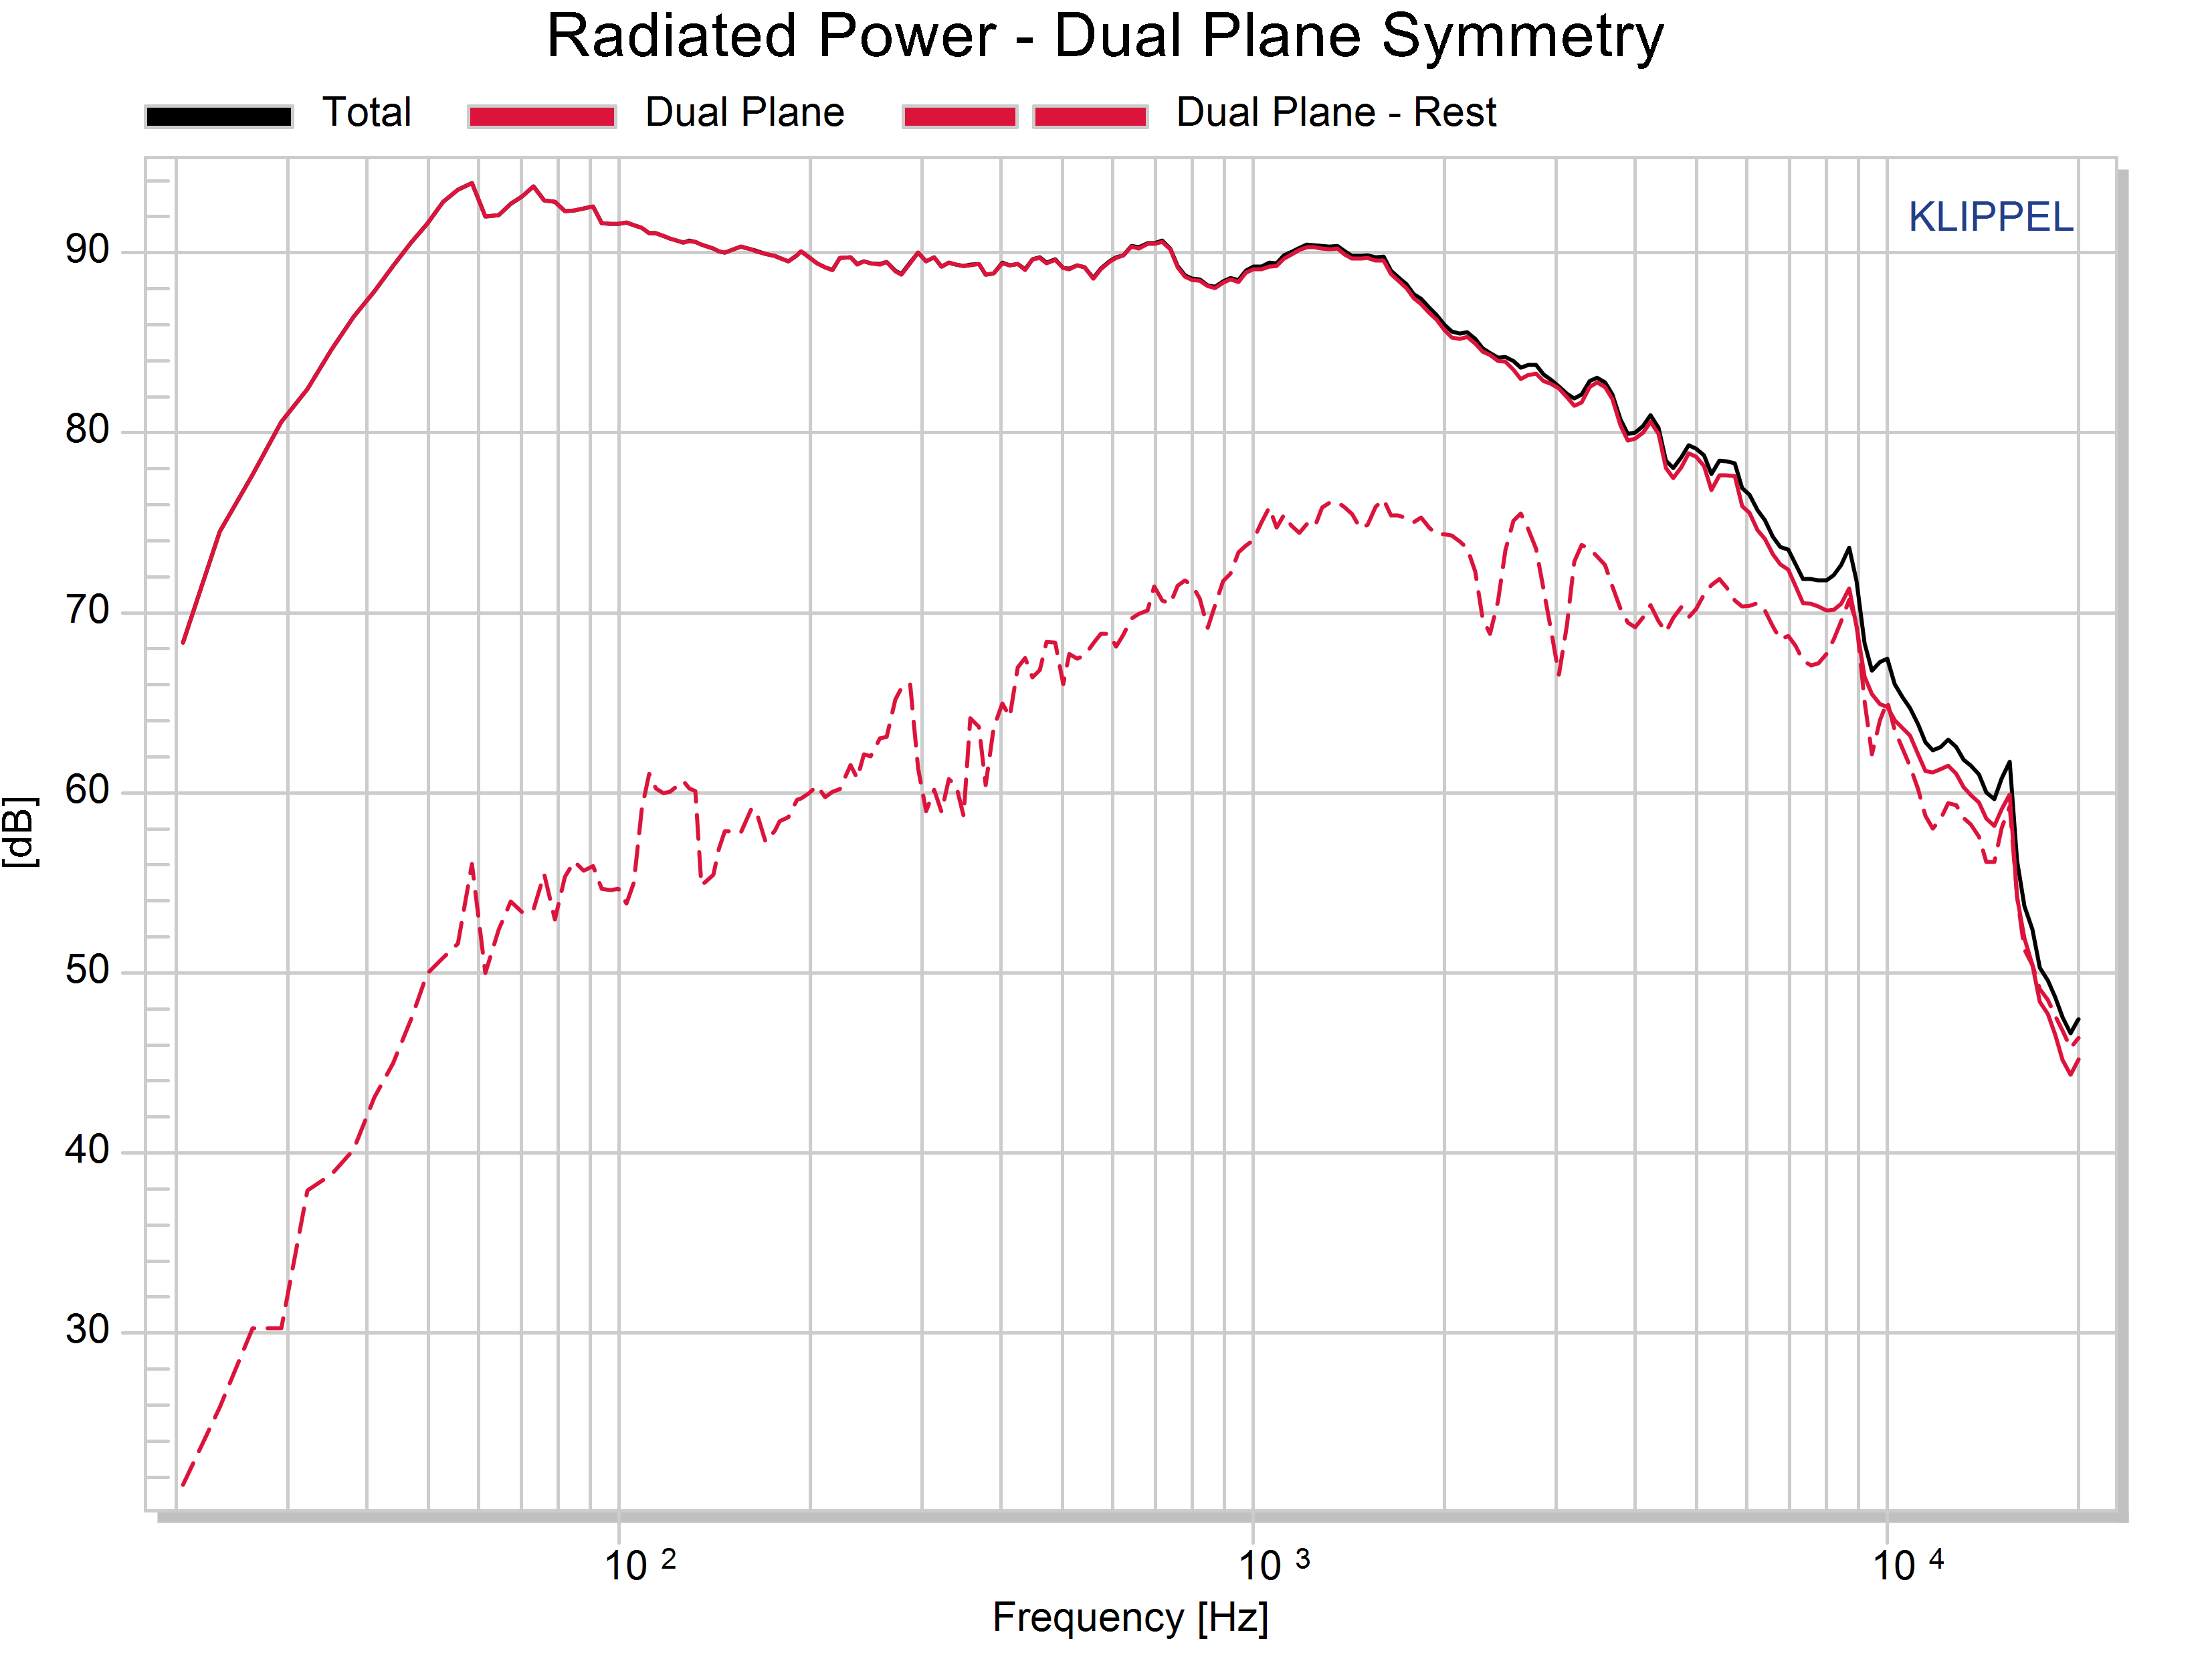
\includegraphics[width=0.9\textwidth]{Sym/Oval_RadPow_Dps}
    \captionsetup{hypcap=false}
    \captionof{figure}{Oval speaker, Radiated Powers: dual plane symmetry}
\end{center}
\end{minipage}

\begin{minipage}{0.5\textwidth}
\begin{center}
	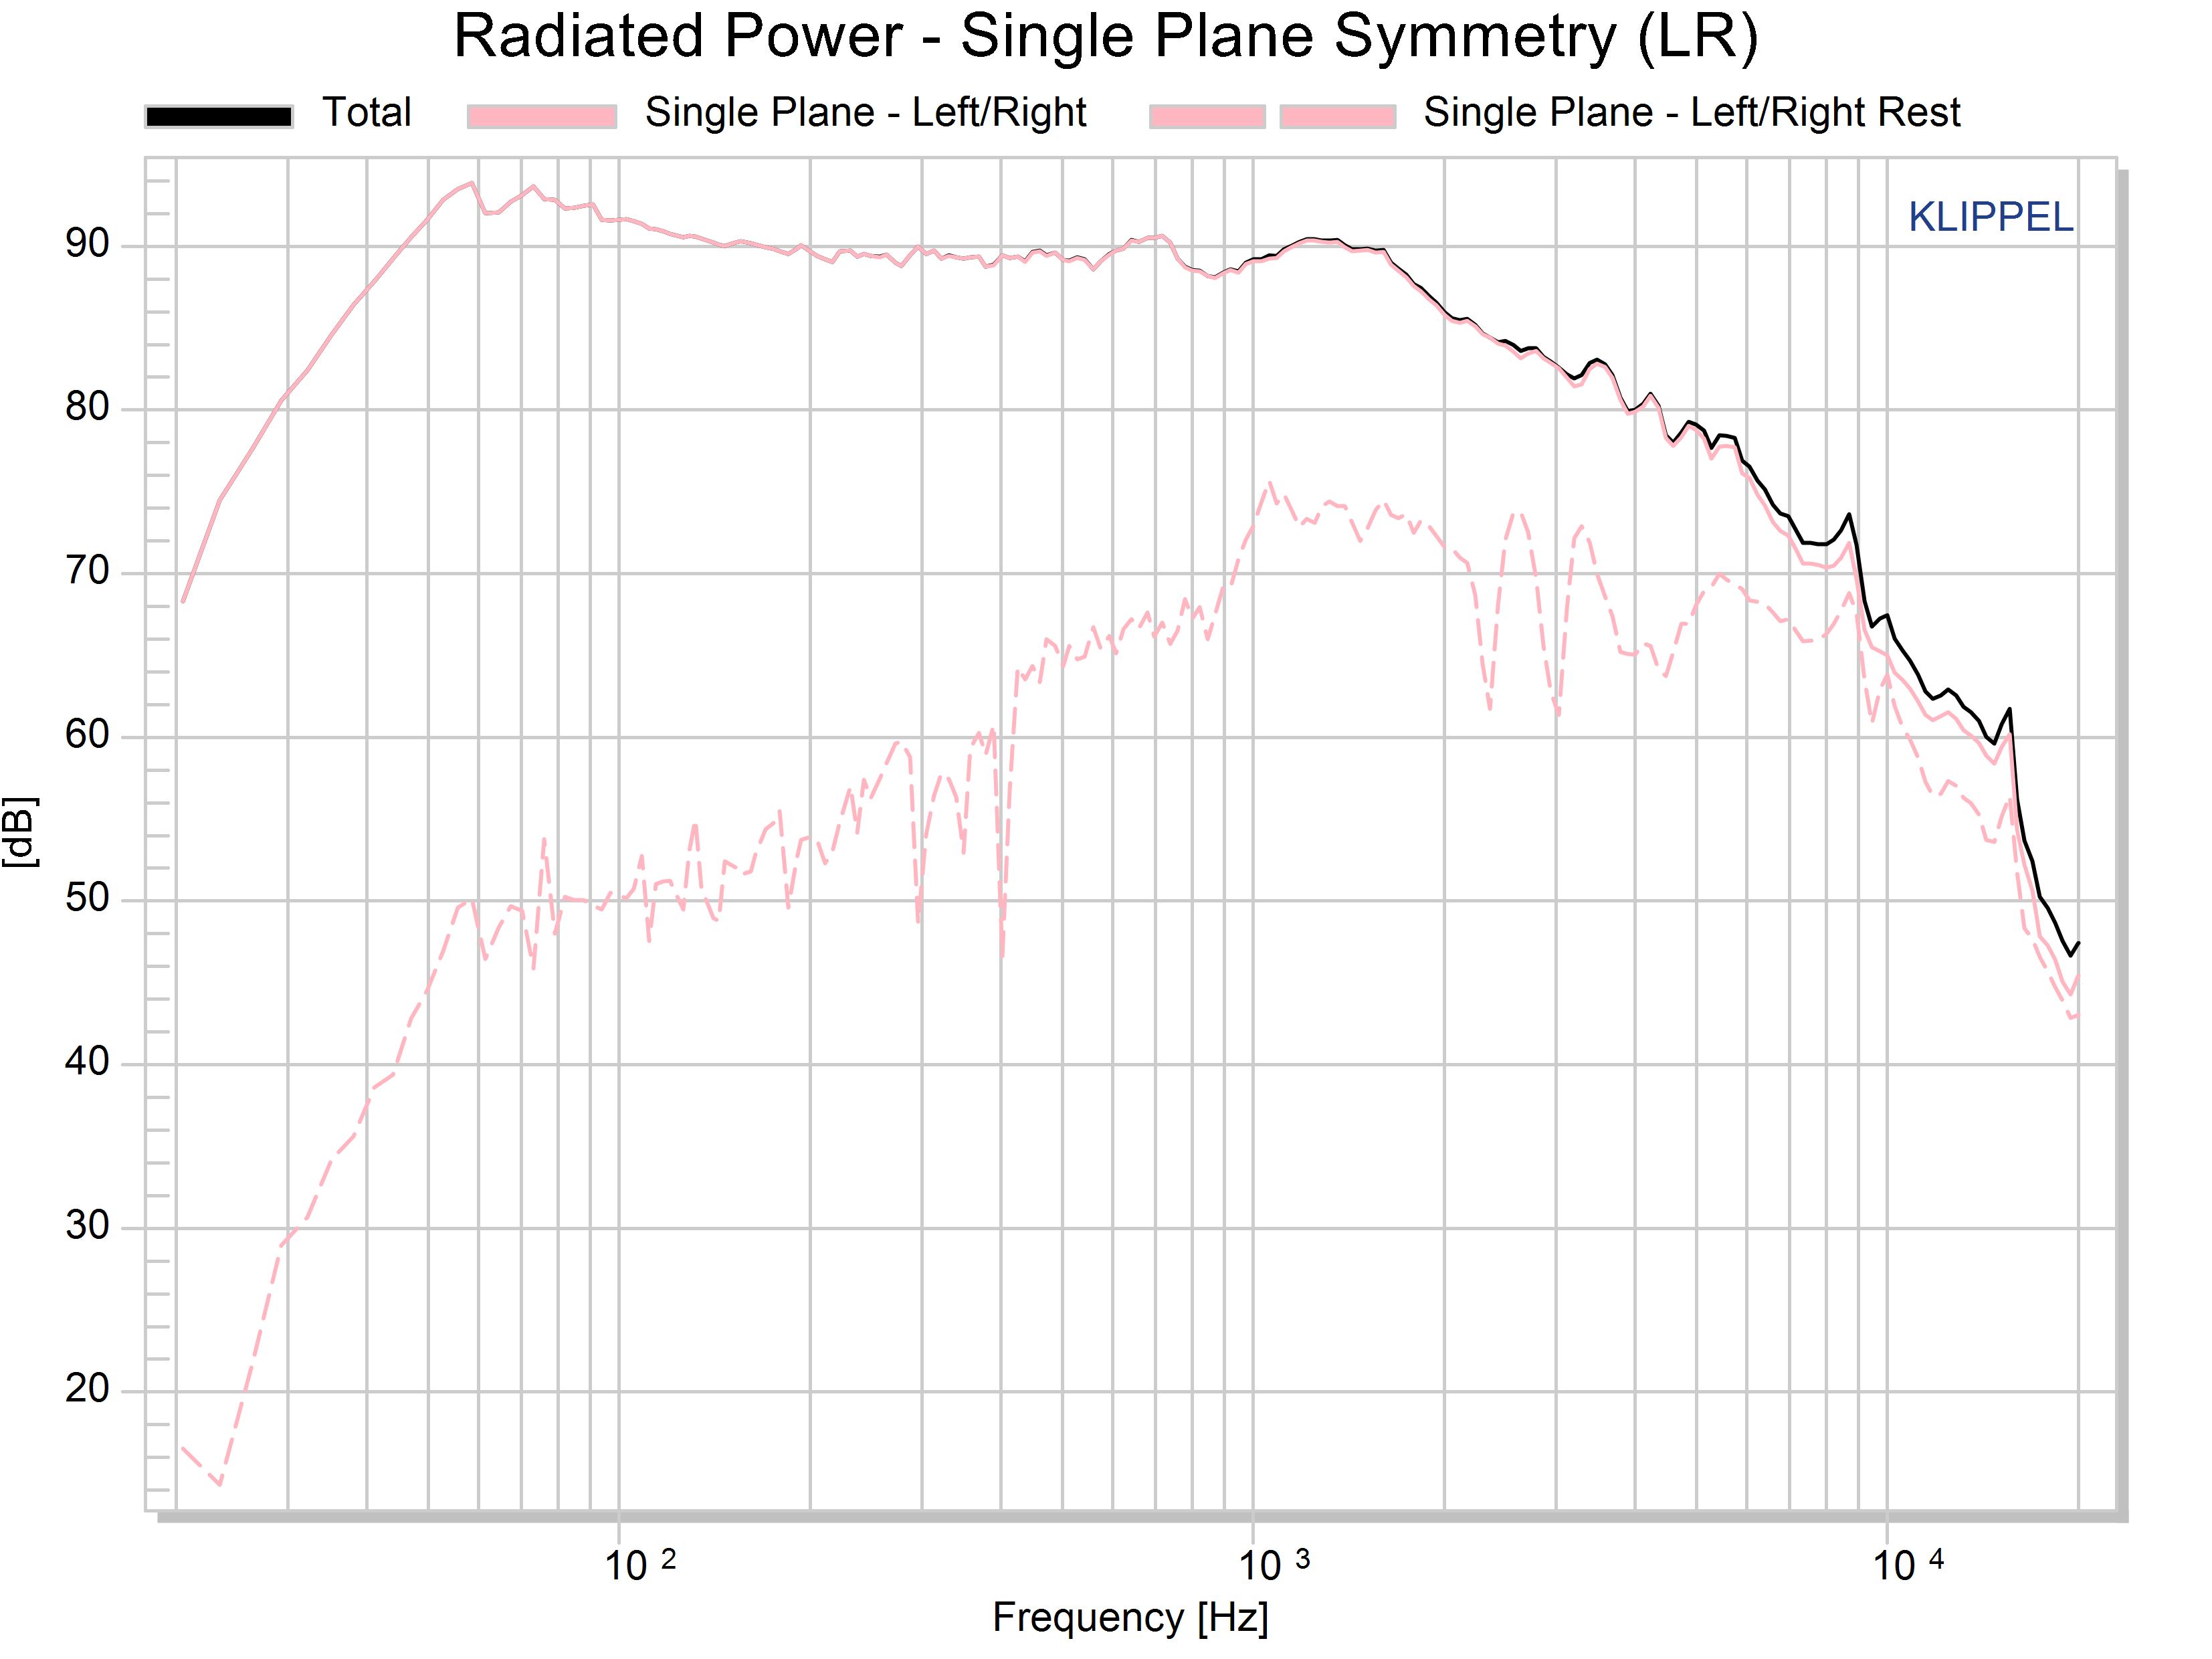
\includegraphics[width=0.9\textwidth]{Sym/Oval_RadPow_SpsLR}
    \captionsetup{hypcap=false}
    \captionof{figure}{Oval speaker, Radiated Powers: single plane (left/right) symmetry}
\end{center}
\end{minipage}
\begin{minipage}{0.5\textwidth}
\begin{center}
	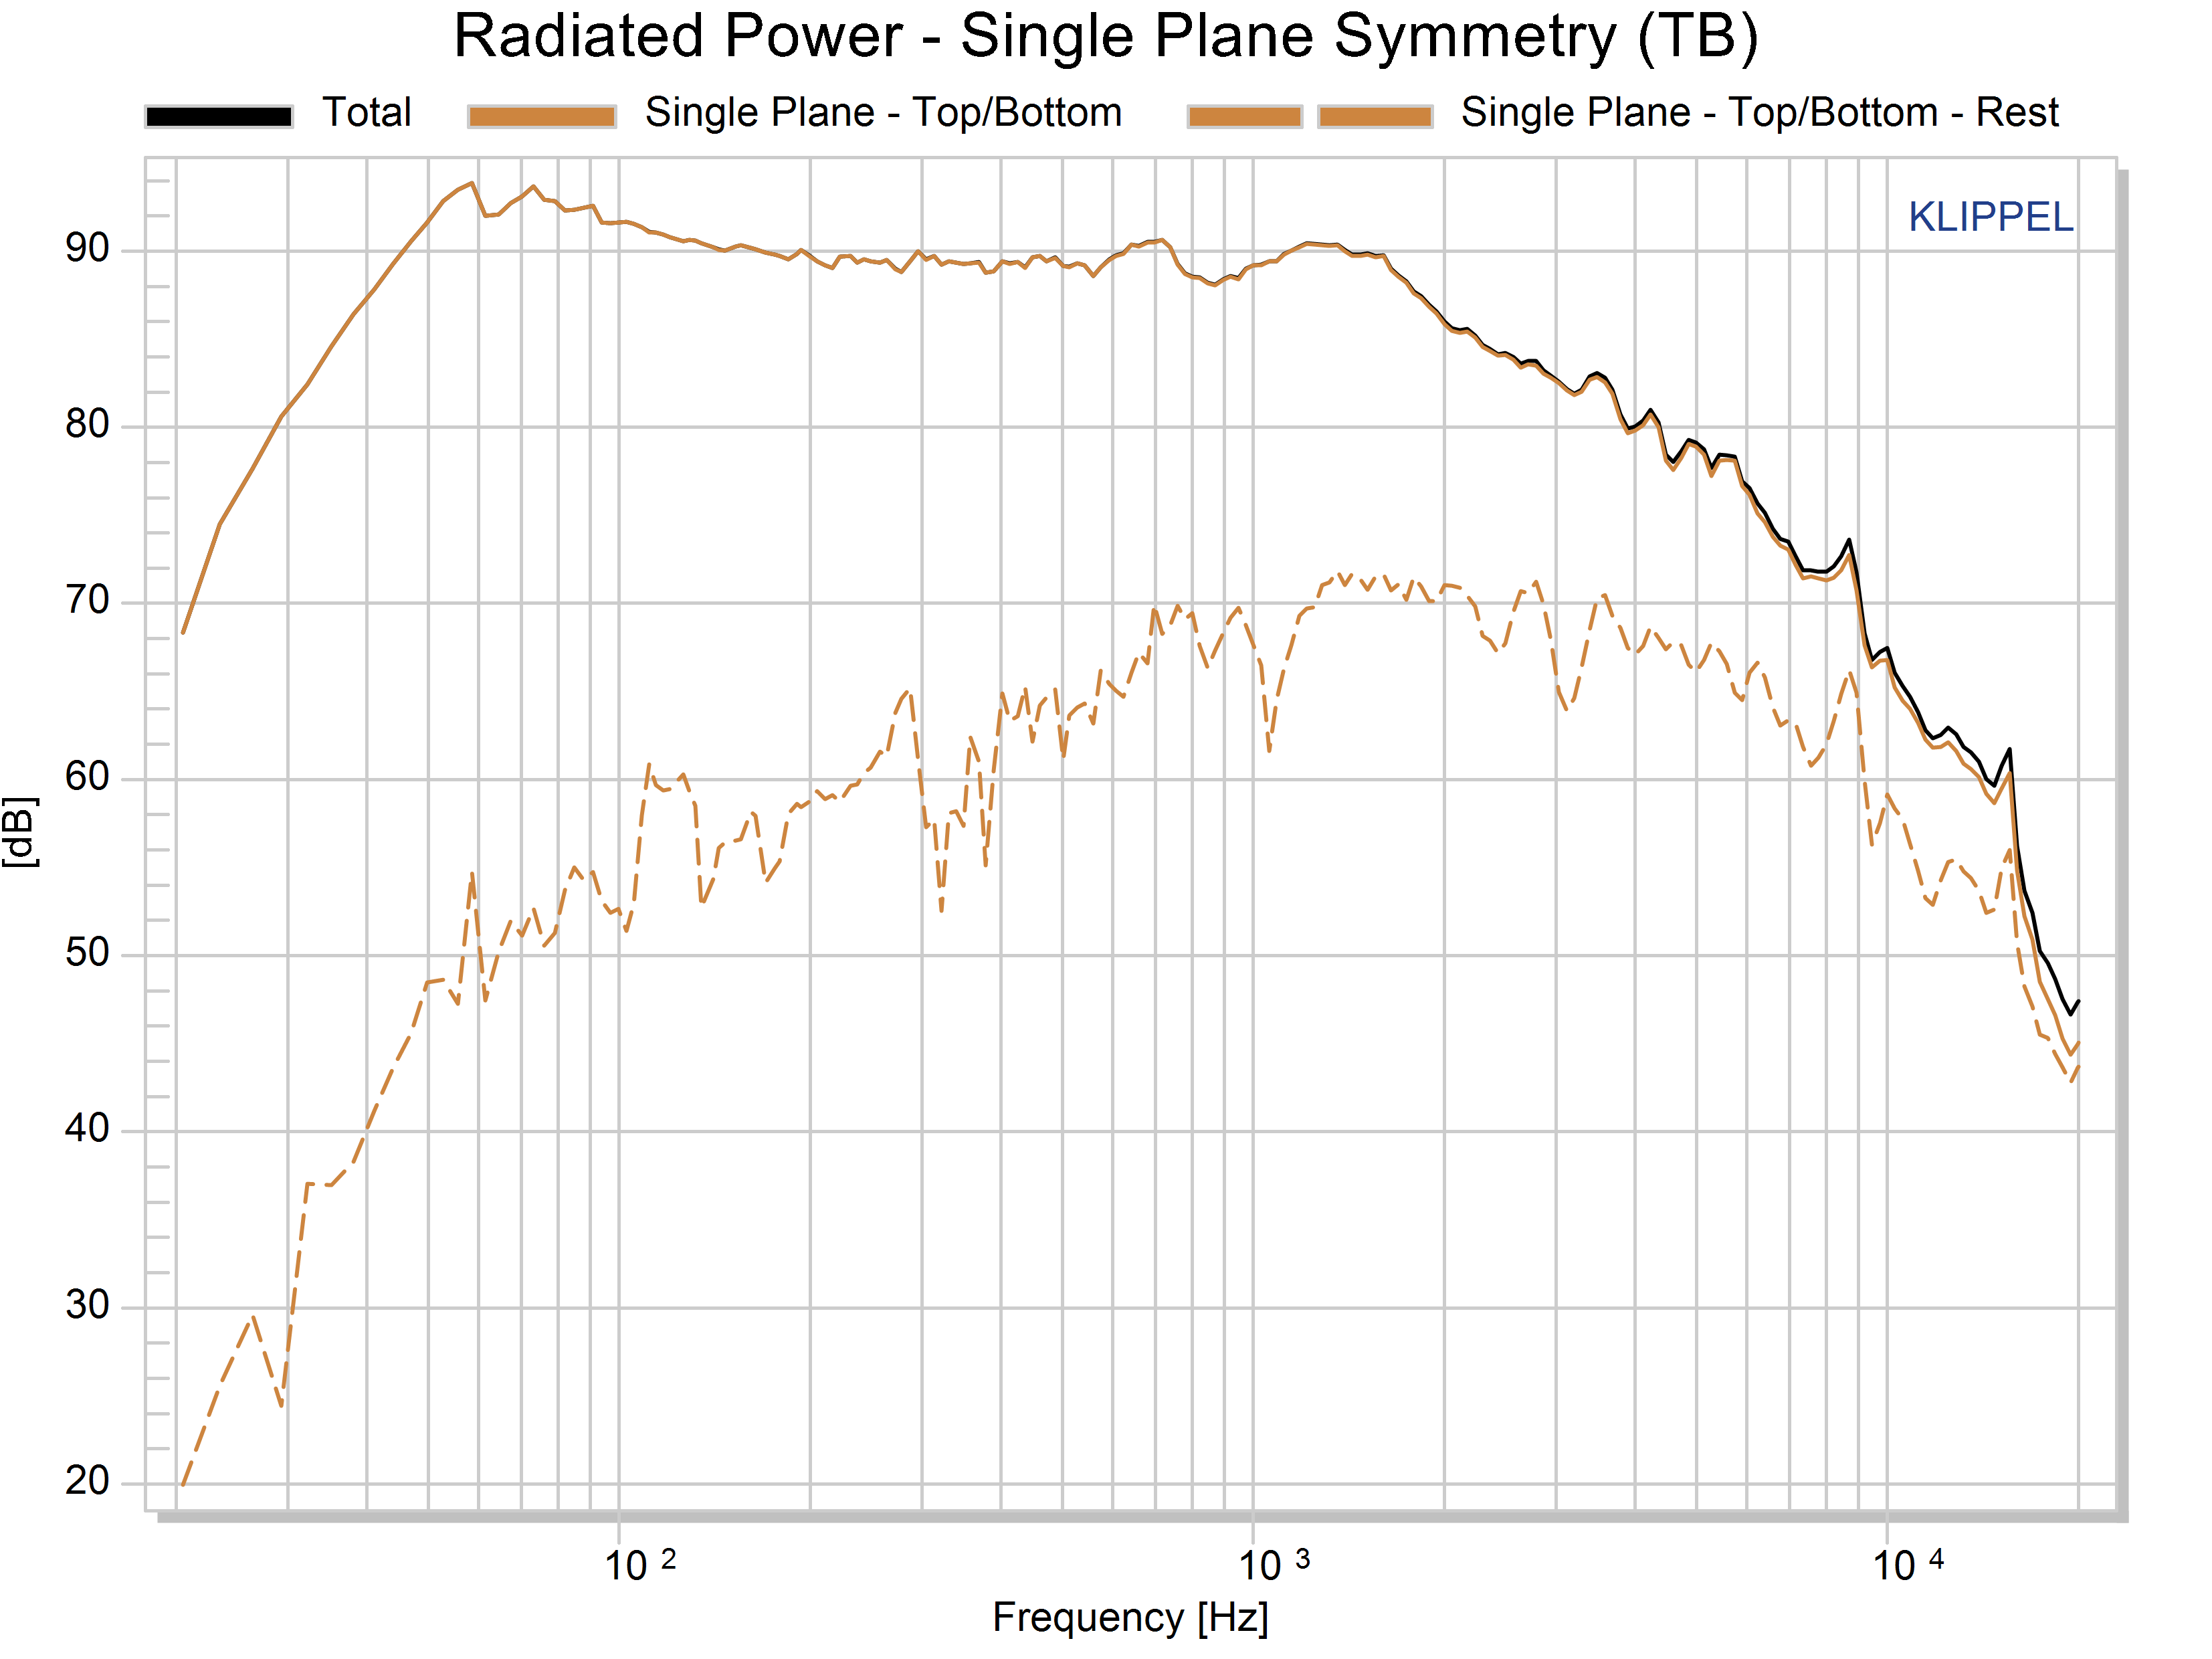
\includegraphics[width=0.9\textwidth]{Sym/Oval_RadPow_SpsTB}
    \captionsetup{hypcap=false}
    \captionof{figure}{Oval speaker, Radiated Powers: single plane (top/bottom) symmetry}
\end{center}
\end{minipage}

\subsection{2-way "diagonal" speaker}
\label{Curves:2way}

\begin{minipage}{0.5\textwidth}
\begin{center}
	\includegraphics[width=\textwidth]{Sym/Contour_BnO}
    \captionsetup{hypcap=false}
    \captionof{figure}{Contour plot of the diagonal speaker at 10 m, centered on-axis, horizontal plane.}
    \label{Curves:2way_contour}
\end{center}
\end{minipage}
\begin{minipage}{0.5\textwidth}
\begin{center}
	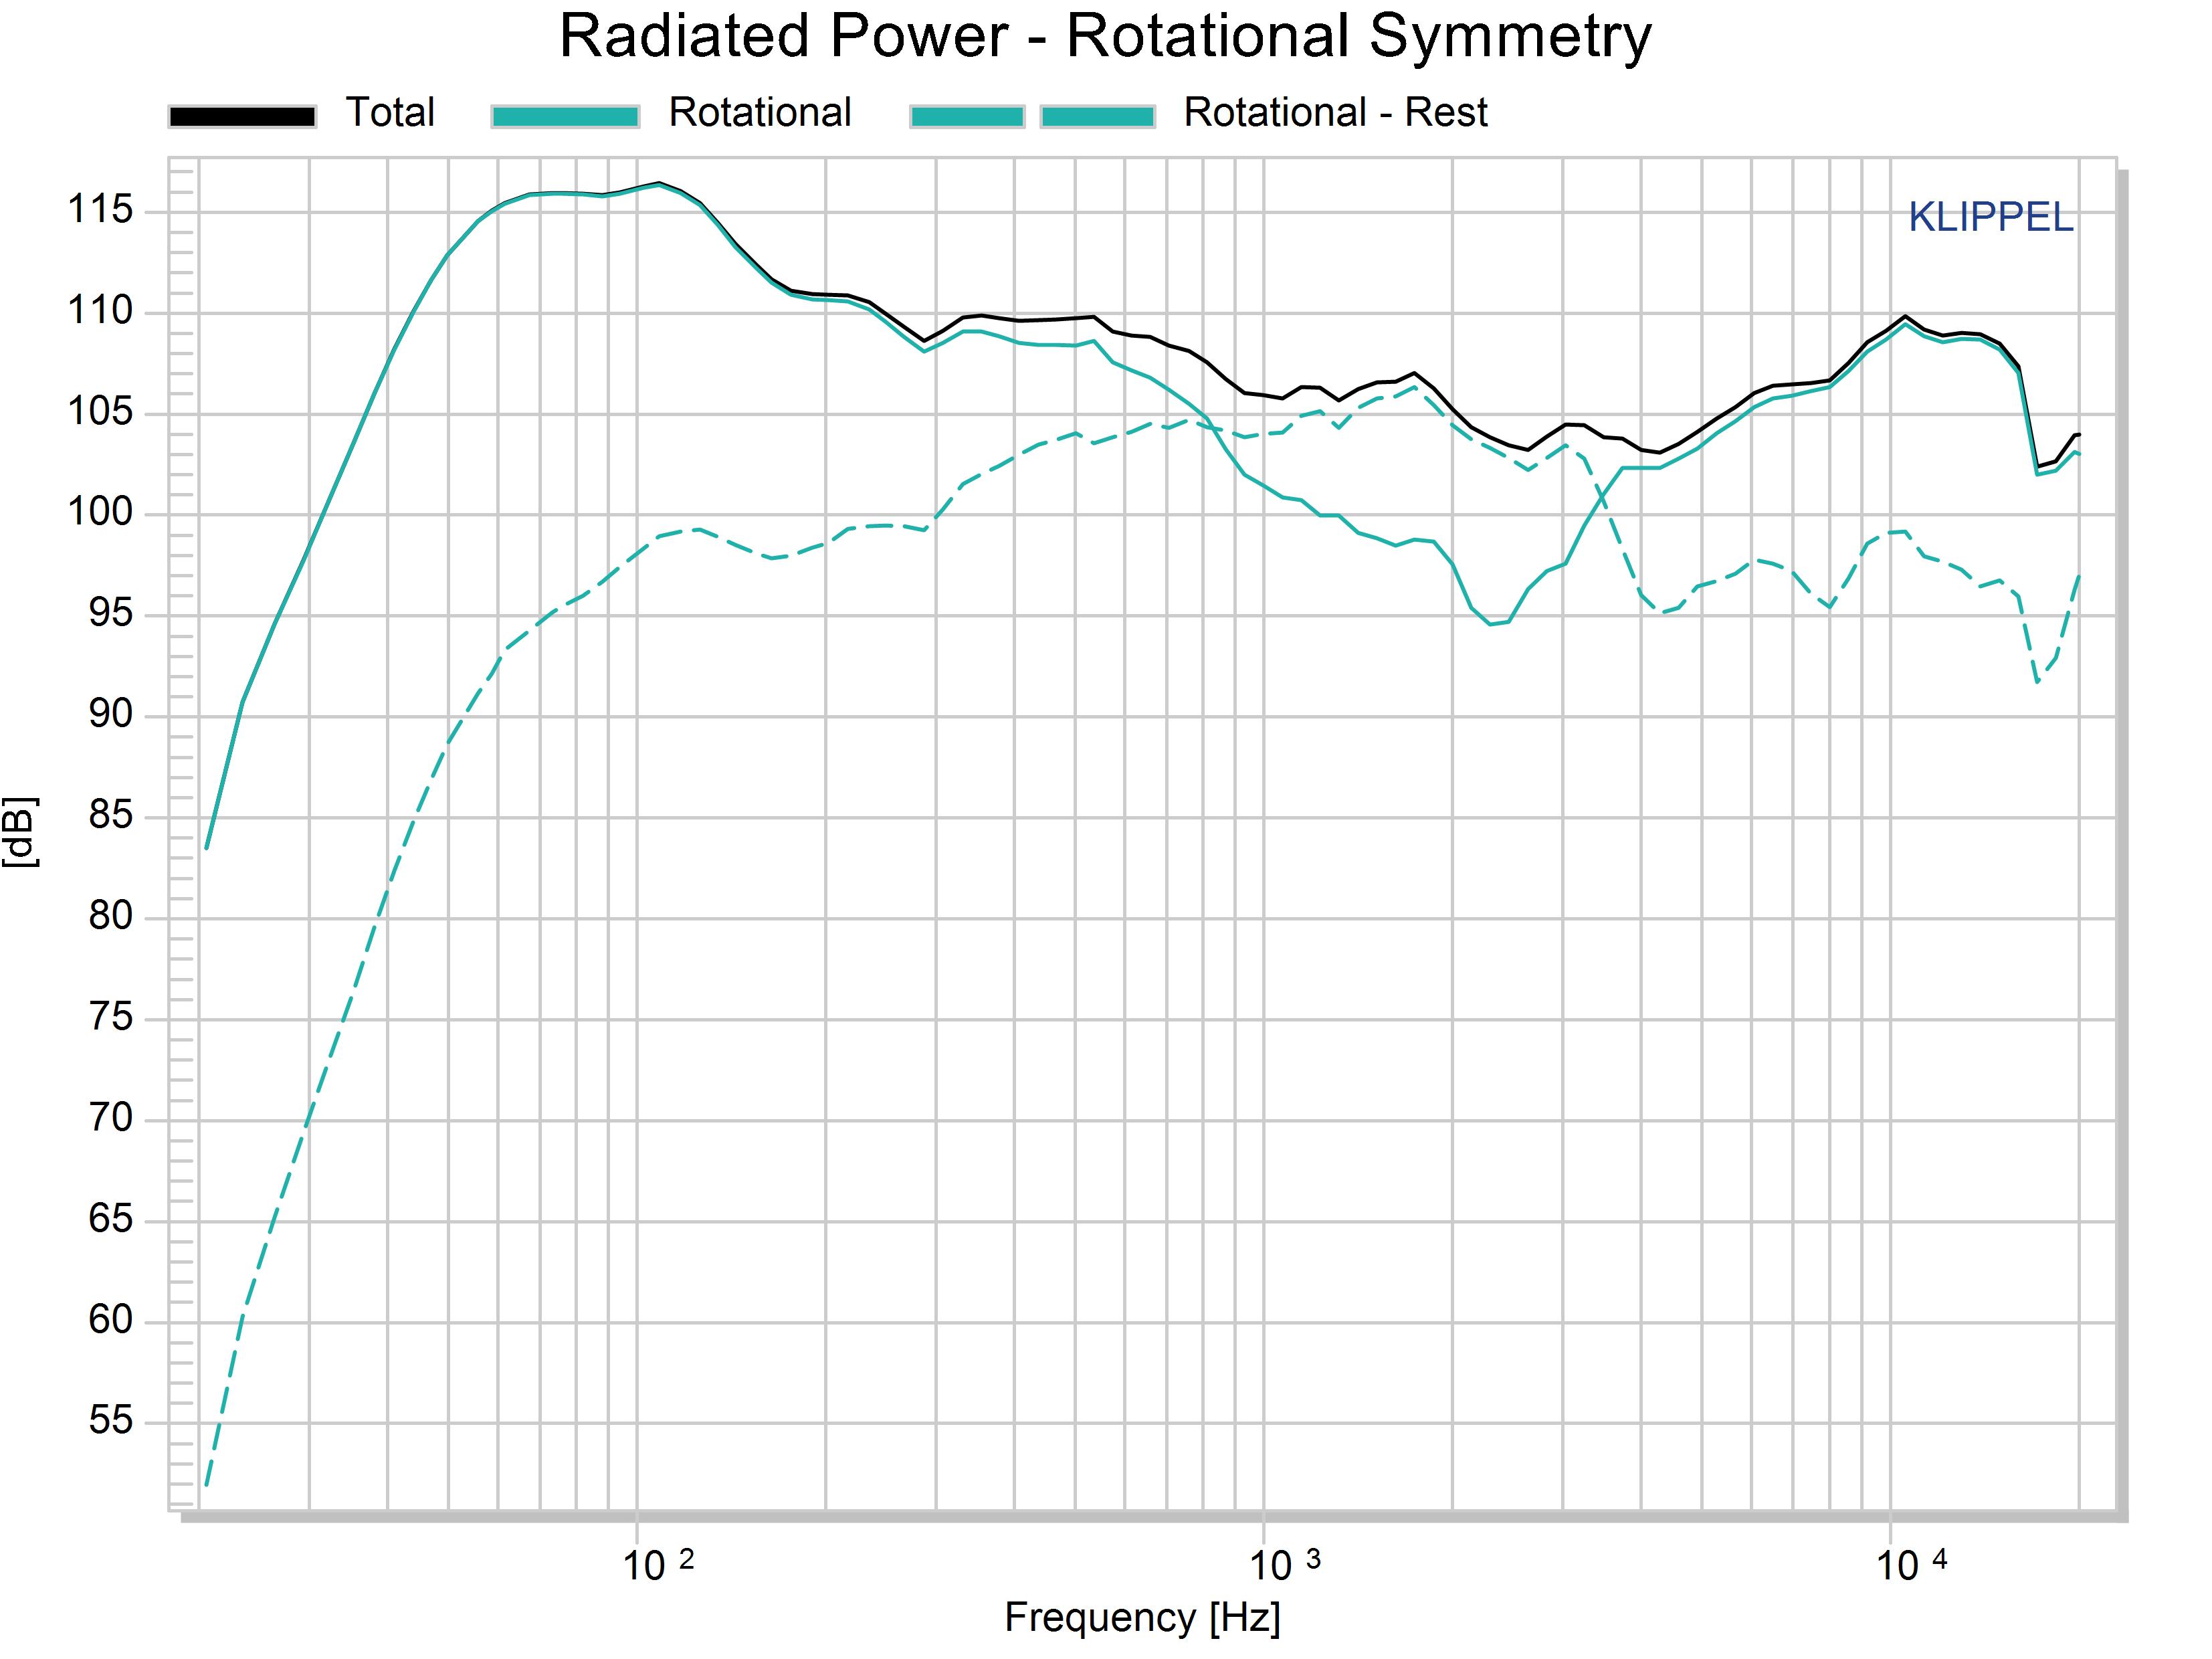
\includegraphics[width=0.9\textwidth]{Sym/BnO_RadPow_Rot}
    \captionsetup{hypcap=false}
    \captionof{figure}{Diagonal speaker, Radiated Powers: rotational symmetry}
\end{center}
\end{minipage}

\begin{minipage}{0.5\textwidth}
\begin{center}
	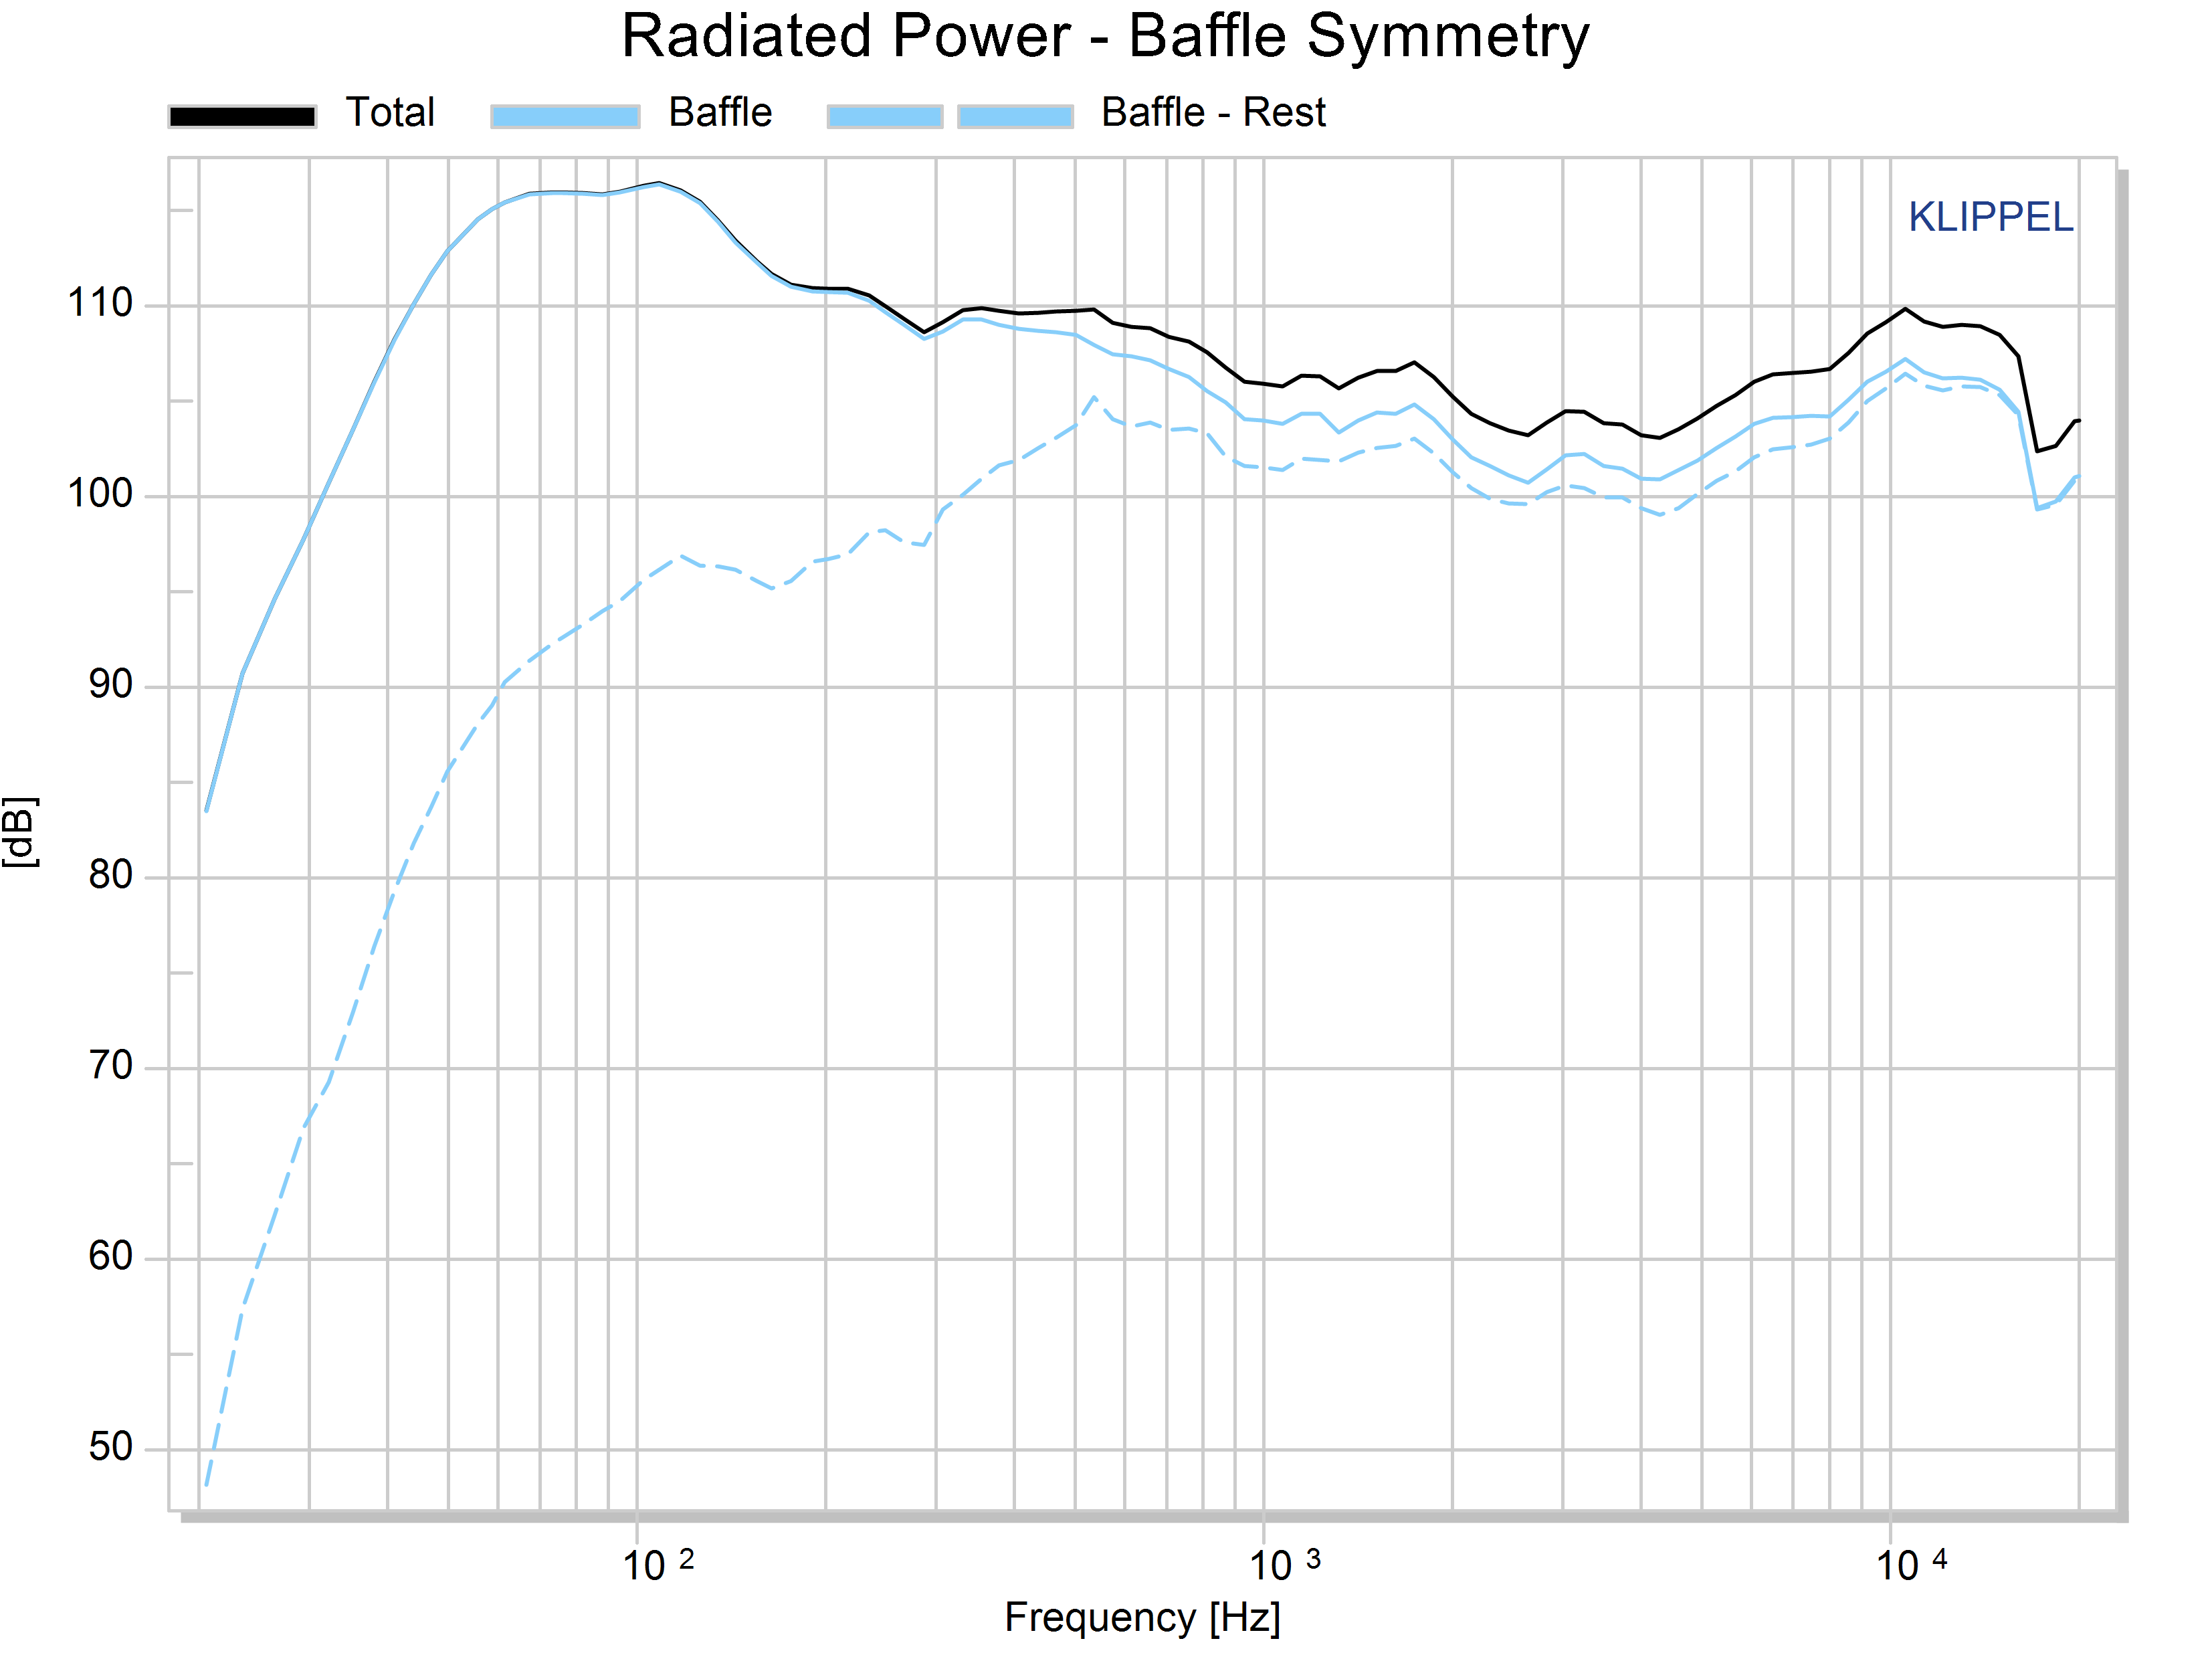
\includegraphics[width=0.9\textwidth]{Sym/BnO_RadPow_B}
    \captionsetup{hypcap=false}
    \captionof{figure}{Diagonal speaker, Radiated Powers: baffle symmetry}
\end{center}
\end{minipage}
\begin{minipage}{0.5\textwidth}
\begin{center}
	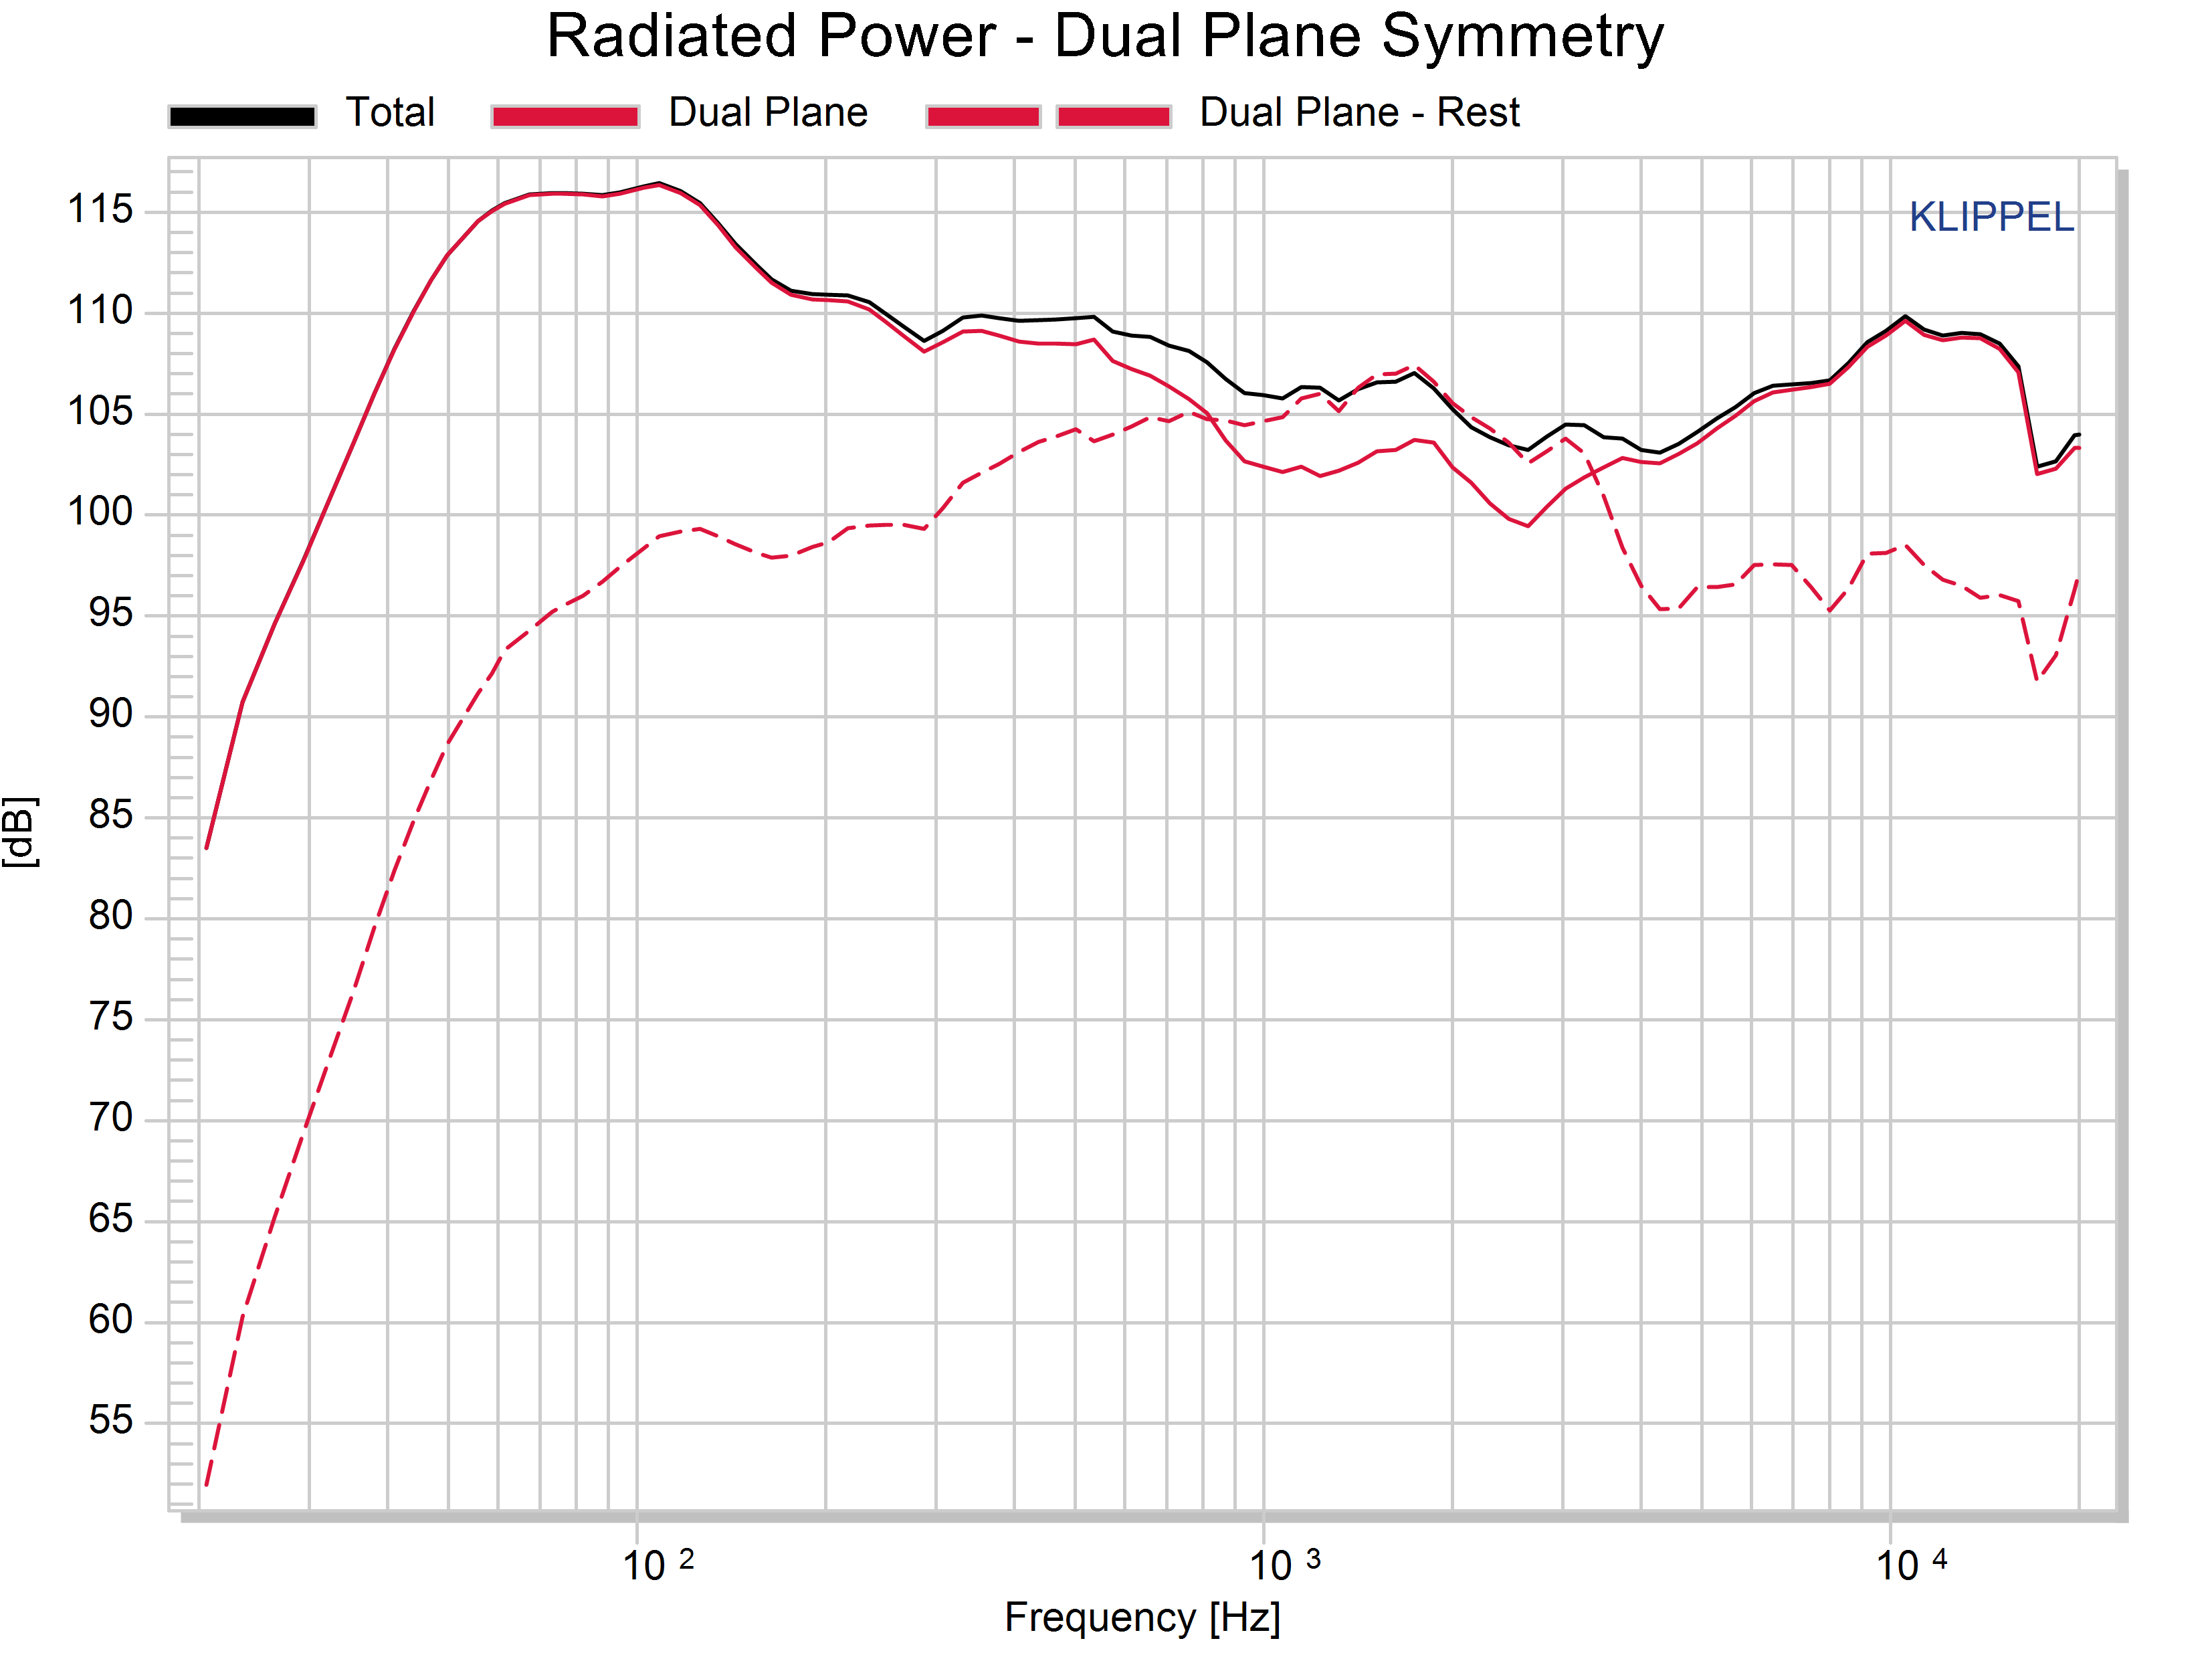
\includegraphics[width=0.9\textwidth]{Sym/BnO_RadPow_Dps}
    \captionsetup{hypcap=false}
    \captionof{figure}{Diagonal speaker, Radiated Powers: dual plane symmetry}
\end{center}
\end{minipage}

\begin{minipage}{0.5\textwidth}
\begin{center}
	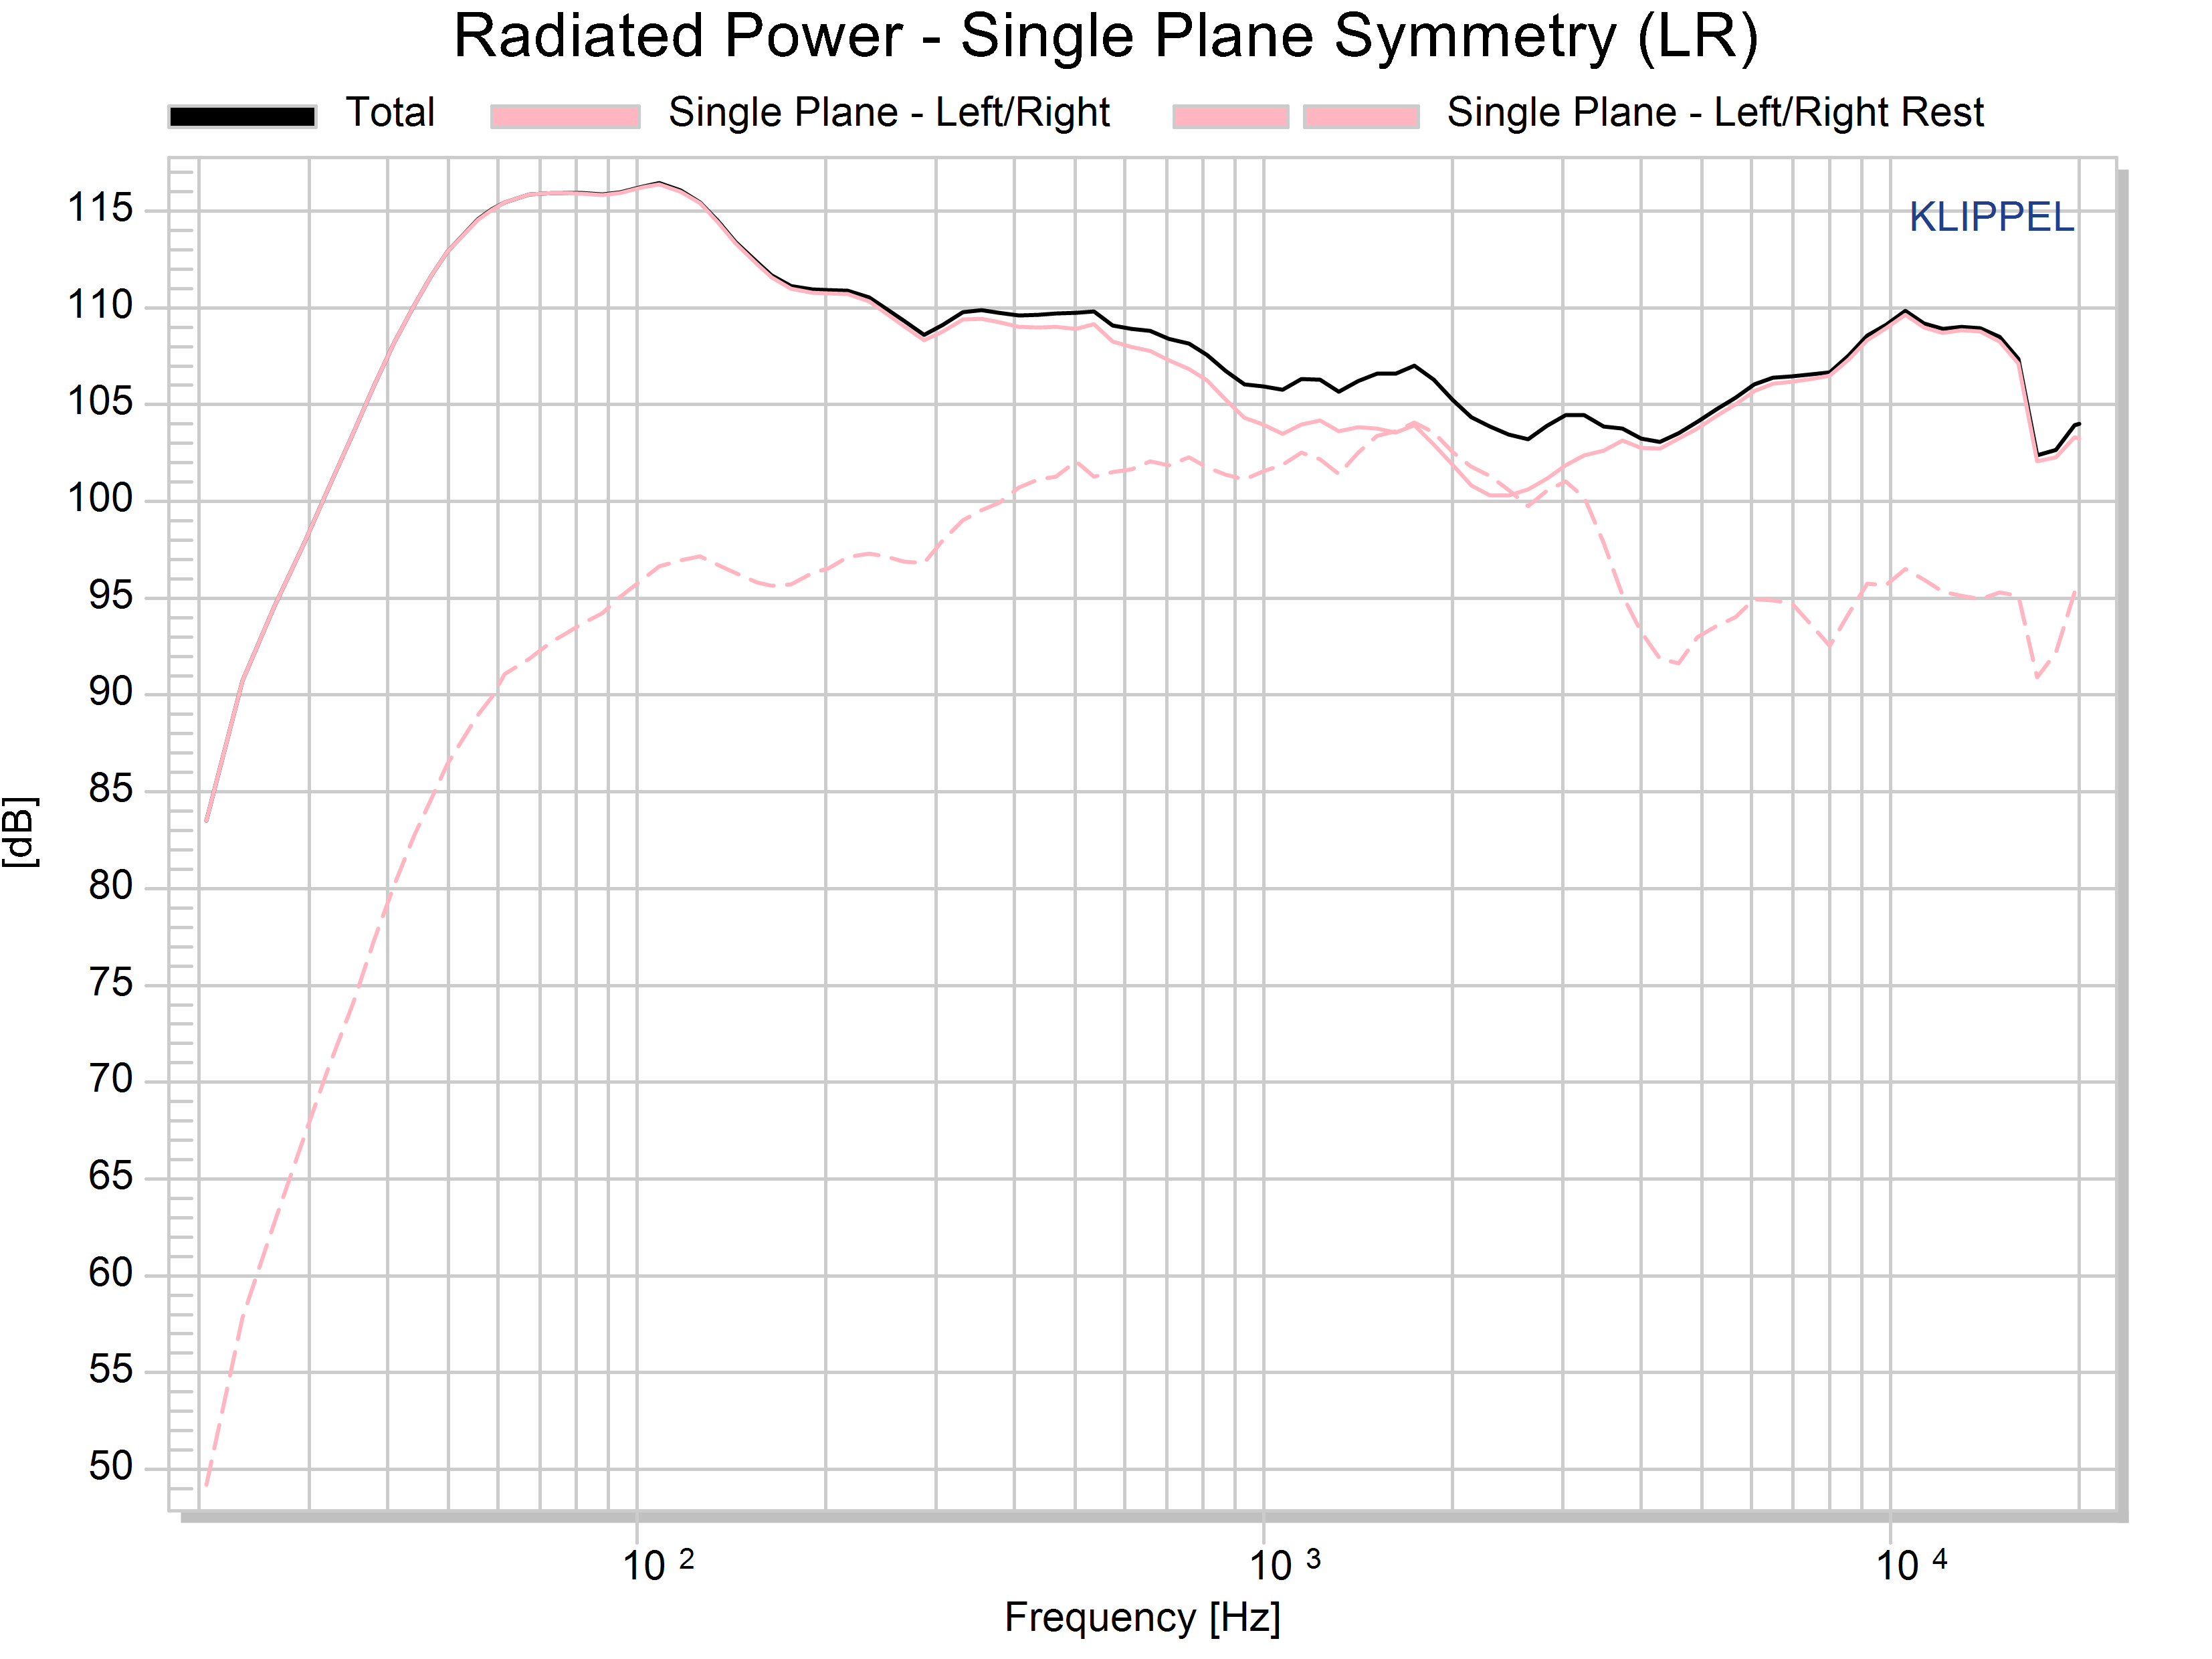
\includegraphics[width=0.9\textwidth]{Sym/BnO_RadPow_SpsLR}
    \captionsetup{hypcap=false}
    \captionof{figure}{Diagonal speaker, Radiated Powers: single plane (left/right) symmetry}
\end{center}
\end{minipage}
\begin{minipage}{0.5\textwidth}
\begin{center}
	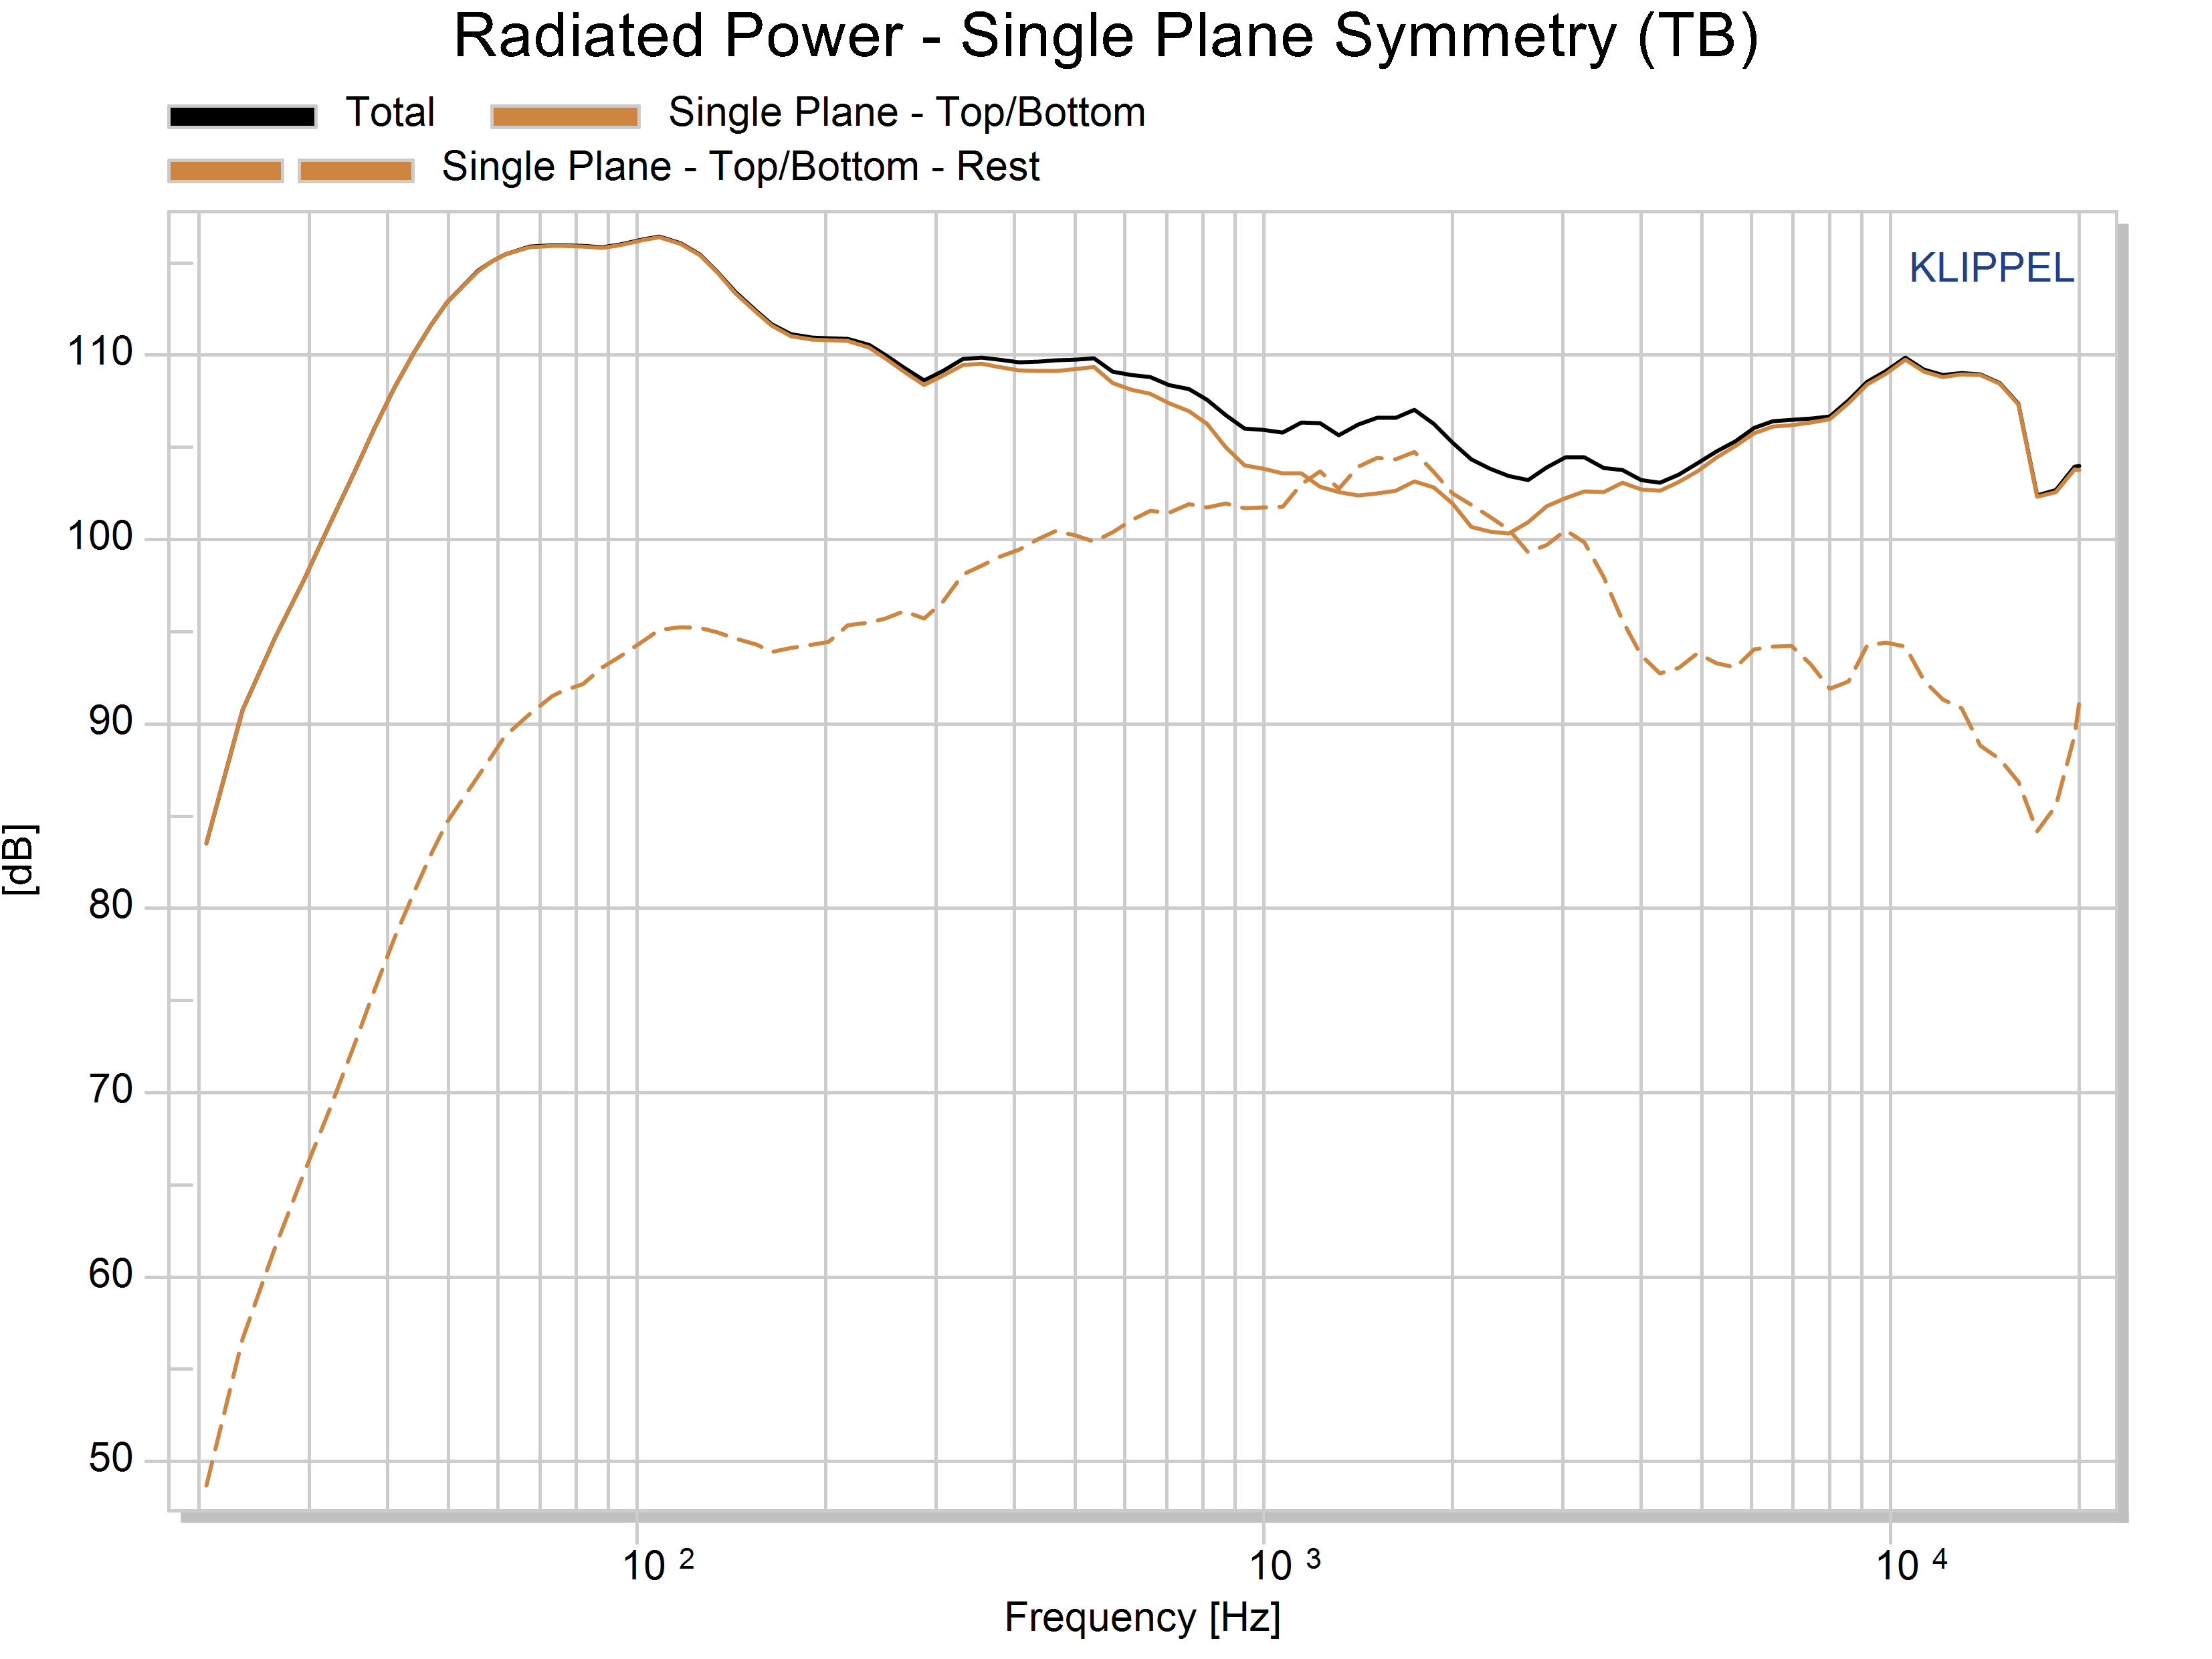
\includegraphics[width=0.9\textwidth]{Sym/BnO_RadPow_SpsTB}
    \captionsetup{hypcap=false}
    \captionof{figure}{Diagonal speaker, Radiated Powers: single plane (top/bottom) symmetry}
\end{center}
\end{minipage}

\subsection{Studio monitor}
\label{Curves:studio}

\begin{minipage}{0.5\textwidth}
\begin{center}
	\includegraphics[width=\textwidth]{Sym/contour_studio}
    \captionsetup{hypcap=false}
    \captionof{figure}{Contour plot of the studio monitor at 10 m, centered on-axis, horizontal plane.}
    \label{Curves:studio_zoom}
\end{center}
\end{minipage}
\begin{minipage}{0.5\textwidth}
\begin{center}
	\includegraphics[width=0.9\textwidth]{Sym/studio_RadPow_Rot}
    \captionsetup{hypcap=false}
    \captionof{figure}{Studio monitor, Radiated Powers: rotational symmetry}
    \label{Curves:studio_rot}
\end{center}
\end{minipage}

\begin{minipage}{0.5\textwidth}
\begin{center}
	\includegraphics[width=0.9\textwidth]{Sym/studio_RadPow_B}
    \captionsetup{hypcap=false}
    \captionof{figure}{Studio monitor, Radiated Powers: baffle symmetry}
    \label{Curves:studio_B}
\end{center}
\end{minipage}
\begin{minipage}{0.5\textwidth}
\begin{center}
	\includegraphics[width=0.9\textwidth]{Sym/studio_RadPow_Dps}
    \captionsetup{hypcap=false}
    \captionof{figure}{Studio monitor, Radiated Powers: dual plane symmetry}
    \label{Curves:studio_Dps}
\end{center}
\end{minipage}

\begin{minipage}{0.5\textwidth}
\begin{center}
	\includegraphics[width=0.9\textwidth]{Sym/studio_RadPow_SpsLR}
    \captionsetup{hypcap=false}
    \captionof{figure}{Studio monitor, Radiated Powers: single plane (left/right) symmetry}
    \label{Curves:studio_SpsLR}
\end{center}
\end{minipage}
\begin{minipage}{0.5\textwidth}
\begin{center}
	\includegraphics[width=0.9\textwidth]{Sym/studio_RadPow_SpsTB}
    \captionsetup{hypcap=false}
    \captionof{figure}{Studio monitor, Radiated Powers: single plane (top/bottom) symmetry}
    \label{Curves:studio_SpsTB}
\end{center}
\end{minipage}

\section{Room Correction}

\subsection{Measurements}

\subsubsection{Influence of the load}
\label{Curves:InfluLoad}

\begin{center}
	\includegraphics[width=0.8\textwidth]{RoomComp/Compa_NFS_BAffle} 
    \captionsetup{hypcap=false} 
	\captionof{figure}{Comparison between the TRF of a measure in baffle and a measure in the box.} 
	\label{fig:Load_Compa}
\end{center}


\subsubsection{Influence of microphone position}
\label{Curves:InfluMicPos}


\begin{center}	
	\includegraphics[scale=0.76,angle=90]{RoomComp/MicPos_TRF} 
	\captionsetup{hypcap=false} 
	\captionof{figure}{Transfer functions for all microphones positions} 
	\label{fig:micpos_TRF_big}
\end{center}

\begin{center}
	\includegraphics[width=0.8\textwidth]{RoomComp/MicPos_Diff_NFS_TRF_zoom} 
    \captionsetup{hypcap=false} 
	\captionof{figure}{Difference between NFS and transfer functions - zoom on 150 Hz - 20 kHz} 
	\label{fig:MicPos_Diff_NFS_Zoom}
\end{center}


\subsection{Room Correction solutions}

\subsubsection{D. B. Keele method for Far Field extrapolation}
\label{Curves:dbkFF}

\begin{center}
	\includegraphics[width=\textwidth]{Appendix/DKeele_FF_All} 
    \captionsetup{hypcap=false} 
	\captionof{figure}[Application of DB Keele method compared with NFS results]{Application of DB Keele method compared with NFS results - Left: shifted curves; Right: non-shifted curves} 
	\label{fig:dbk_fig}
\end{center}


		% Symmetry

\chapter[Equations for symmetry condition on complex coefficients of spherical wave expansion]{Equations for symmetry condition on complex \\ coefficients of spherical wave expansion}
\label{chap:sym}

\textit{\textbf{NOTE}: the presented equations are coming from the reference \cite{aeshs}. They are displayed in this report for a more comfortable reading experience and for reference, and I do not take any credits for the presented results.} \\

\begin{minipage}{0.5\textwidth}
\begin{center}
	\includegraphics[scale=0.25]{Appendix/Spherical_Harmo}
    \captionsetup{hypcap=false}
    \captionof{figure}{Spherical Harmonics}
    \label{fig:Sph_Harmo}
\end{center}
\end{minipage}
\begin{minipage}{0.5\textwidth}
\vspace{0.2cm}
The solution of the three-dimensional wave equation in spherical coordinates can be described by a spherical wave expansion given by equation \ref{eq:sphwvexp}.The free-field transfer function of a loudspeaker can be expressed by only considering the direct sound (outgoing wave) in equation \ref{eq:sphwvexp} and is expressed in equation \ref{eq:ffHf}.\\

Figure \ref{fig:Sph_Harmo} presents a visual representation of the first few spherical harmonics, and their orders (n,m) (\textit{all images presented in this chapter are courtesy of W. Klippel, from the presentation \cite{lect2018}}). \\~\\~\\~\\
\end{minipage}

\textbf{Influence of symmetry on coefficients} \\

\begin{minipage}{0.7\textwidth}
Rotational symmetry (see figure \ref{fig:rotsym}) is observed for many circular drivers and is the simplest type of symmetry as a lot of coefficients are vanishing according to the relation given by equation \ref{eq:Crotsym}.

\begin{equation}
C_{mn} = 0 \; \; \; \;  m \neq 0
\label{eq:Crotsym}
\end{equation}
\myequations{Coefficients for rotational symmetry}
All m $\neq$ 0 coefficients are vanishing, meaning that only m = 0, n = n+1 coefficients have to be estimated. \\

Once the coefficients have been estimated, s symmetry factor S can be estimated. For rotation symmetry, $S_{rs}$ is given by equation \ref{eq:Srs}.

\begin{equation}
S_{rs} = 1-\frac{\sum_{n=1}^{N}\sum_{s=1}^{n}\left | C_{sn} \right |^{2}}{\sum_{n=0}^{N}\sum_{m=-n}^{n} C_{mn}^{2}}
\label{eq:Srs}
\end{equation}
\myequations{Symmetry factor for rotational symmetry}

\end{minipage}
\begin{minipage}{0.3\textwidth}
\begin{center}
	\includegraphics[width=\textwidth]{Appendix/Rot_Sym}
    \captionsetup{hypcap=false}
    \captionof{figure}{Rotational symmetry}
    \label{fig:rotsym}
\end{center}
\end{minipage}

\begin{minipage}{0.7\textwidth}
Dual plane symmetry (see figure \ref{fig:dualpsym}) is mostly observed in 2-way closed box systems, and make half of the coefficients vanish according to the relation given by equation \ref{eq:Cdpsym}. 

\begin{equation}
C_{mn}(f) = C_{-mn}(f)R_{m}(f) \; \; \; \;  m = 2s; \; s =1, 2, 3...
\label{eq:Cdpsym}
\end{equation}
\myequations{Coefficients for dual plane symmetry}
Where Rm represents a complex symmetry parameter, expressed in equation \ref{eq:Rm}.

\begin{equation}
R_{m}(f) = (-1)^{m+1}(\textup{sin}(m \phi _{s}(f)) + i\textup{cos}(m \phi _{s}(f)))^{2}
\label{eq:Rm}
\end{equation}
\myequations{Complex symmetry parameter}
With $\phi _{s}$ is the symmetry axis; and $m$ the suborder of the coefficient under study.
\end{minipage}
\begin{minipage}{0.3\textwidth}
\begin{center}
	\includegraphics[width=\textwidth]{Appendix/Dual_Plane_Sym}
    \captionsetup{hypcap=false}
    \captionof{figure}{Dual Plane symmetry}
    \label{fig:dualpsym}
\end{center}
\end{minipage}\\


If the symmetry axes $\Phi _{e}, \Theta _{e}$ are aligned with the coordinate system, equation \ref{eq:Cdpsym} can be simplified to the relation given in equation \ref{eq:Cdpsymb}.

\begin{equation}
C_{mn}(f) = C_{-mn}(f) \; \; \; \;  m = 2s; \; s =1, 2, 3...
\label{eq:Cdpsymb}
\end{equation}
\myequations{Coefficients for dual plane symmetry}
The symmetry factor for the Dual Plane symmetry is then given by equation \ref{eq:Sdps}.


\begin{equation}
S_{dps} = 1-\frac{\sum_{n=1}^{N}\sum_{s=1}^{n/2}\left | (-1)^{2s}C_{(2s)n} - C_{(2s)n}\right |^{2} + \sum_{n=1}^{N}\sum_{s=0}^{n/2}\left | C_{(2s+1)n}\right |^{2}}{\sum_{n=0}^{N}\sum_{m=-n}^{n} C_{mn}^{2}}
\label{eq:Sdps}
\end{equation}
\myequations{Symmetry factor for dual-plane symmetry}

\vspace{1cm}

\begin{minipage}{0.7\textwidth}
Baffle symmetry is when the Device Under Test is mounted on a baffle (see figure \ref{fig:bafflesym}), and make half of the coefficient vanish according to the relation given by equation \ref{eq:Cbsym}.

\begin{equation}
C_{mn} = 0 \; \; \; \; \; \; n-m \, \neq \, 2s; \: \: s \in \mathbb{Z}
\label{eq:Cbsym}
\end{equation}
\myequations{Coefficients for baffle symmetry}
The symmetry factor is then given by equation \ref{eq:Sbs}.

\begin{equation}
S_{bs} = 1-\frac{\sum_{n=1}^{N}\sum_{s=0}^{n/2}\left | C_{(2s)n} \right |^{2}}{\sum_{n=0}^{N}\sum_{m=-n}^{n} C_{mn}^{2}}
\label{eq:Sbs}
\end{equation}
\myequations{Symmetry factor for baffle symmetry}
\end{minipage}
\begin{minipage}{0.3\textwidth}
\begin{center}
	\includegraphics[width=\textwidth]{Appendix/Baffle_Sym}
    \captionsetup{hypcap=false}
    \captionof{figure}{Baffle symmetry}
    \label{fig:bafflesym}
\end{center}
\end{minipage}

\vspace{1cm}

\begin{minipage}{0.7\textwidth}
Single plane symmetry is the most common in loudspeaker systems using 2 or more drivers. This symmetry can be between the left and right side of the DUT, as presented in figure \ref{fig:singplsym}; but also between the top and bottom of the DUT. Only the coefficients on the left side have to be estimated. The coefficients of the right side are linked to the left side by the relation given by equation \ref{eq:spsym}.

\begin{equation}
C_{mn} = C_{-mn}(f)R_{m}(f) \; \; \; \textup{with} \; \; m\geq 0; \; \; \; 0\leq n\leq N
\label{eq:spsym}
\end{equation}
\myequations{Coefficients for single plane symmetry}
It should be noted that depending of the type of symmetry (left/right or top/bottom), $R_{m}$ will change, modifying the relation between the coefficients. \\

The symmetry factor is then given by equation \ref{eq:Ssps}.

\begin{equation}
S_{sps} = 1-\frac{\sum_{n=1}^{N}\sum_{m=1}^{n}\left | (-1)^{m}(f) C_{-mn}-C_{mn} \right |^{2}}{\sum_{n=0}^{N}\sum_{m=-n}^{n} C_{mn}^{2}}
\label{eq:Ssps}
\end{equation}
\myequations{Symmetry factor for single plane symmetry}
\end{minipage}
\begin{minipage}{0.3\textwidth}
\begin{center}
	\includegraphics[width=\textwidth]{Appendix/Single_Plane_Sym}
    \captionsetup{hypcap=false}
    \captionof{figure}{Single Plane symmetry}
    \label{fig:singplsym}
\end{center}
\end{minipage}

\newpage

\textbf{Implementation} \\

The following code shows how these equations have been implemented in SciLab.\\
\textit{\textbf{NOTE}: This program have been simplified by removing some functions, the aim being to demonstrate how the algorithm calculating the coefficients based on symmetry conditions works.}

\lstset{language=SCilab} 
\begin{lstlisting}
//------------------------------------------------MAIN FUNCTION
function OnRun()
// Loading the datas
Cout = load('Cout.txt');
Cin  = load('Cin.txt');
f    = load('f.txt');

N = sqrt(size(Cout,1))-1; // Number of points

// Constants 
P0  = 10^(-12);		      //reference sound power
rho = 1.204;		         //density of the air
c   = 343;		            //speed of sound
k   = 2*%pi*f'/c;	         //wavenumber k
A   = 4*%pi*radius^2; 

// Rotational symmetry (example)
[Csym_ROT, Crest_DPS, powOut_rot, powRestOut_rot] = CheckSymAll(Cout, N, f, 'ROT');
ROT_TotOut_FF  = [f' 10*log10(powOut_rot' ./(rho*c*k^2)/P0)];        // Total outgoing power 
ROT_OutRest_FF = [f' 10*log10(powRestOut_rot' ./(rho*c*k^2)/P0)];    // Rest of outgoing power
ROT_SymFactor_FF = [f' (abs(powOut_rot./(powOut_rot+powRestOut_rot)))'];    // Symmetry factor
endfunction // OnRun

//--------------------------------------------Find the coeffs for different symmetries
function [Csym, Crest, power_sym, power_rest] = CheckSymAll(C, N, f, SymType)
   // CheckSymAll: calculates the coeff according the different symmetry conditions
   // Inputs:     C: coefficients to find symmetry on 
   //             N: number of iterations 
   //             f: frequency vector
   //             SymType: a string with the symmetry types. 
   //	          Allowed values are: 'ROT', 'DPS', 'BS', 'SPS_LR', 'SPS_TB' 
   //                      representing respectively Rotational Symmetry, Dual Plane Symmetry, 
   //                      Baffle Symmetry, Single Plane Symmetry (Left/Right),
   //					   Single Plane Symmetry (Top/Bottom).
   // Outputs:    Csym: coefficients of the symmetry condition
   //             Crest: rest of coefficients = all coeffs - Csym
   //             power_sym: power of the symmetry coefficients
   //             power_rest: power of the rest coeffcients   
   
   // Initialization of matrices (all coeffs, left and right coefficients)
   Csym = zeros(size(C,'r'),size(C,'c'));
   Csym_l = zeros(size(C,'r'),size(C,'c'));  
   Csym_r = zeros(size(C,'r'),size(C,'c'));
   
   // Calculation of coefficient according to symmetry condition assumed
   select SymType
   case 'ROT' 
      [nm] = calc_nm_index(N*ones(f), 1);                      
      [n, m] = order_suborder(nm(:,1));   // Finding the equivalent n and m values   
      
      // Finding the equivalent index value for m=0
      index = GetIndex(n, m);      
      Csym(index,:) = C(index,:);   // If m=0 we put the value in C in the Csym
      // Calculation of rest 
      Crest = C - Csym;
   case 'DPS'
      [nm] = calc_nm_index(N*ones(f), 5);                
      [n, m] = order_suborder(nm(:,1));   // Finding the equivalent n and m values
      index_row = GetIndex(n, m);

      Csym_l(index_row,:) = C(index_row,:);  // Filling the Coeffs of the left with the correct data
      
      // Finding the equivalent m value for the right side
      for i = 1:size(m,'r')
         m_r(i) = -1*m(i);
         index_r(i) = GetIndex(n(i), m_r(i));
         index_l(i) = GetIndex(n(i), m(i));
         if isequal(index_l(i),index_r(i))==%F then
            Csym_r(index_r(i),:) = (1)*C(index_l(i),:);
         end
      end
      Csym = Csym_l + Csym_r;
      // Calculation of rest 
      Crest = C - Csym;
   case 'BS'
      [nm] = calc_nm_index(N*ones(f), 2);    // For baffle
      [n, m] = order_suborder(nm(:,1));   // Finding the equivalent n and m values      
      index_row = GetIndex(n, m);                // Index of relevant rows for the Coeffs         
      Csym(index_row,:) = C(index_row,:);  
      // Calculation of rest 
      Crest = C - Csym;
   case 'SPS_LR'
      [nm] = calc_nm_index(N*ones(f), 4);         // Indexes of left side
      [n, m] = order_suborder(nm(:,1));   // Finding the equivalent n and m values
      index_left = GetIndex(n, m);
            
      m_right = -1.*m;                          // Indexes of right side
      weights = ((-1)^(m));
      index_right = GetIndex(n, m_right);
      
      [nm] = calc_nm_index(N*ones(f), 1);         // Indexes of middle (m=0)
      [n, m] = order_suborder(nm(:,1));   // Finding the equivalent n and m values
      index_middle = GetIndex(n, m);
      
      Csym_l(index_left,:) = C(index_left,:);      
      for i=1:size(C,'c')
         Csym_r(index_right,i) = Csym_l(index_left,i).*weights;   // Weighting the coefficients
      end
      Csym_m(index_middle,:) = C(index_middle,:);      
      Csym_r2(index_right,:) = C(index_right,:);
      for i=1:size(C,'c')
         Csym_l2(index_left,i) = Csym_r2(index_right,i)./weights;
      end 
      
      avg_Left = (Csym_l + Csym_l2)/2;
      avg_Right = (Csym_r + Csym_r2)/2;
      Csym = Csym_m + avg_Left + avg_Right;
      Crest = C - Csym;
   case 'SPS_TB'
      [nm] = calc_nm_index(N*ones(f), 4);         // Indexes of left side
      [n, m] = order_suborder(nm(:,1));   // Finding the equivalent n and m values
      index_left = GetIndex(n, m);
      
      m_right = -1*m;
      index_right = GetIndex(n, m_right);
      
      [nm] = calc_nm_index(N*ones(f), 1);         // Indexes of middle (m=0)
      [n, m] = order_suborder(nm(:,1));   // Finding the equivalent n and m values
      index_middle = GetIndex(n, m);
      
      Csym_l(index_left,:) = C(index_left,:);
      Csym_r(index_right,:) = Csym_l(index_left,:);   // No weighting is needed for the T/B symmetry
      Csym_m(index_middle,:) = C(index_middle,:);      
      Csym_r2(index_right,:) = C(index_right,:);
      Csym_l2(index_left,:) = Csym_r2(index_right,:);
      
      avg_Left = (Csym_l + Csym_l2)/2;
      avg_Right = (Csym_r + Csym_r2)/2;      
      Csym = Csym_m + avg_Left + avg_Right;
      Crest = C - Csym;
   end
   
   // Calculation of power
   power_sym  = sum(abs(Csym).^2,1);    // Estimating the power of sym
   power_rest = sum(abs(Crest).^2,1);   // Estimating the power of rest
endfunction
\end{lstlisting}

		% Speaker library
\chapter{Speaker library}
\label{chap:spk_lib}

\section{10 cm woofer}
\label{spkrlib:10cm}

\begin{minipage}{0.6\textwidth}
This speaker is a 10 cm (4'') woofer from PSS, designed for automotive applications. A picture is shown in figure \ref{fig:spkr_lib_10cm}\\ 
The Thiele \& Small  parameters of this speaker have been measured using the Klippel scanning system and are presented in table \ref{tab:TnS_10cmWoofer}. 
\end{minipage}
\begin{minipage}{0.4\textwidth}
\begin{center}
	\includegraphics[scale=1]{Appendix/Round_Spkr}
    \captionsetup{hypcap=false}
    \captionof{figure}{10 cm woofer}
    \label{fig:spkr_lib_10cm}
\end{center}
\end{minipage}




\begin{table}[ht]
\centering
\begin{tabular}{|c|c|c|c|c|c|c|c|c|c|}
\hline
\begin{tabular}[c]{@{}c@{}}Re \\{[}$\Omega${]}\end{tabular} & \begin{tabular}[c]{@{}c@{}}Fs\\{[}Hz{]}\end{tabular} & \begin{tabular}[c]{@{}c@{}}Mms\\  {[}g{]}\end{tabular} & \begin{tabular}[c]{@{}c@{}}Cms\\{[}mm/N{]}\end{tabular} & \begin{tabular}[c]{@{}c@{}}Rms\\  {[}kg/s{]}\end{tabular} & Bl    & Qms   & Qes   & Qts   & \begin{tabular}[c]{@{}c@{}}Vas\\  {[}L{]}\end{tabular} \\ \hline
3.28                                                                        & 145.8                                                                 & 5.492                                                                 & 0.217                                                                    & 1.619                                                                    & 3.197 & 3.108 & 1.614 & 1.063 & 1.89                                                                  \\ \hline
\end{tabular}
\caption{T \& S parameters of 10cm woofer}
\label{tab:TnS_10cmWoofer}
\end{table}

\section{Oval speaker}
\label{spkrlib:oval}

\begin{minipage}{0.6\textwidth}
This speaker is a 23 cm x 15 cm fullband speaker. A picture is shown in figure \ref{fig:spkr_lib_Oval}.\\
The T\&S parameters of the speaker were not given and haven't been measured.

\end{minipage}
\begin{minipage}{0.4\textwidth}
\begin{center}
	\includegraphics[scale=1]{Appendix/Oval_Spkr}
    \captionsetup{hypcap=false}
    \captionof{figure}{Oval speaker}
    \label{fig:spkr_lib_Oval}
\end{center}
\end{minipage}

\section{16 cm fullband speaker}
\label{spkrlib:12cm}

This speaker is a 16 cm fullband speaker. The T\&S parameters are given in table \ref{tab:TnS_FullBand}.

\begin{table}[ht]
\centering
\begin{tabular}{|c|c|c|c|c|c|c|c|c|c|}
\hline
\begin{tabular}[c]{@{}c@{}}Re \\ {[}$\Omega${]}\end{tabular} & \begin{tabular}[c]{@{}c@{}}Fs\\{[}Hz{]}\end{tabular} & \begin{tabular}[c]{@{}c@{}}Mms\\  {[}g{]}\end{tabular} & \begin{tabular}[c]{@{}c@{}}Cms\\ {[}mm/N{]}\end{tabular} & \begin{tabular}[c]{@{}c@{}}Rms\\  {[}kg/s{]}\end{tabular} & Bl    & Qms   & Qes   & Qts   & \begin{tabular}[c]{@{}c@{}}Vas\\  {[}L{]}\end{tabular} \\ \hline
5.39                                                                        & 52                                                                    & 14.630                                                                & 0.641                                                                    & 0.724                                                                    & 8.112 & 6.599 & 0.391 & 0.369 & 11.6093                                                               \\ \hline
\end{tabular}
\caption{T\&S parameters of 12cm fullband driver}
\label{tab:TnS_FullBand}
\end{table}

\section{2-way diagonal speaker}
\label{spkrlib:BnO}

\begin{minipage}{0.6\textwidth}
This 2-way speaker presents the particularity of having its tweeter and woofer mounted diagonally as shown by figure \ref{fig:2wayDiagSpkr}. The measurements have been focused on the tweeter of this speaker, and the reference axis for the measure have been setted along the "measurement axis" showed on the side view in figure \ref{fig:2wayDiagSpkr}.

\end{minipage}
\begin{minipage}{0.4\textwidth}
\begin{center}
	\includegraphics[scale=0.2]{Sym/Spkr_BmO}
    \captionsetup{hypcap=false}
    \captionof{figure}{2-way diagonal speaker}
    \label{fig:2wayDiagSpkr}
\end{center}
\end{minipage}

\section{Studio Monitor}
\label{sprklib:Studio}

\begin{minipage}{0.6\textwidth}
This system is a 2-way studio monitor, presented in figure \ref{fig:StudioMon}. Its crossover frequency is 2 kHz.

\end{minipage}
\begin{minipage}{0.4\textwidth}
\begin{center}
	\includegraphics[scale=0.05]{Appendix/Studio}
    \captionsetup{hypcap=false}
    \captionof{figure}{Studio monitor}
    \label{fig:StudioMon}
\end{center}
\end{minipage}


\section{18'' woofer}

\begin{minipage}{0.6\textwidth}
This speaker is an 18'' JBL WPU1805-X woofer. The T\&S parameters were provided by the manufacturer and are presented in table \ref{tab:TnS_BigBooy}. 
\begin{center}
\begin{tabular}{|c|c|c|c|c|c|}
	\hline
	\begin{tabular}[c]{@{}c@{}}Re \\ {[}$\Omega${]}\end{tabular} & \begin{tabular}[c]{@{}c@{}}Fs\\  {[}Hz{]}\end{tabular} & 	Qms   & Qes  & Qts & \begin{tabular}[c]{@{}c@{}}Vas\\  {[}L{]}\end{tabular} \\ \hline
	5.6                                                          & 35                                                     & 	21.09 & 0.73 &  0.70   & 293                                                    \\ \hline
\end{tabular}
\captionsetup{type=table} \caption{T\&S parameters of 18'' woofer}
\label{tab:TnS_BigBooy}
\end{center}
\end{minipage}
\begin{minipage}{0.4\textwidth}
\begin{center}
	\includegraphics[width=0.6\textwidth]{Appendix/bigwoof}
    \captionsetup{hypcap=false}
    \captionof{figure}{18'' woofer}
    \label{fig:bigwoof}
\end{center}
\end{minipage}


		% GANTT CHART
\chapter{Organization of the work}
\pagenumbering{roman}

The following will present the work schedule I have followed, what work have been done and when it have been started and finished. This is presented in the following GANTT chart.

\begin{center}
	\includegraphics[width=\textwidth]{Appendix/Plan1} 
\end{center}


		% More baffle prototype images
\chapter{Baffle Prototype pictures}

\missingfigure{Prendre des photos du proto}

		% Application Notes
\chapter{Application notes}

\section{Baffle measurement}
\label{chap:AN_Baffle}


\section{Complex Room Compensation module}
\label{chap:AN_CRC}


\end{appendices}

\end{document}
